\documentclass[a4paper,10pt]{article}
\usepackage[utf8]{inputenc}
\usepackage{amsmath}
\usepackage{fullpage}
\usepackage{hyperref}
\usepackage{cleveref}
\usepackage{graphicx}
\usepackage{listings}
\usepackage{color}
\usepackage{float}
\usepackage{apacite}

\definecolor{mygreen}{rgb}{0,0.6,0}
\definecolor{mygray}{rgb}{0.5,0.5,0.5}
\definecolor{mymauve}{rgb}{0.58,0,0.82}

\lstset{ 
  backgroundcolor=\color{white},   % choose the background color; you must add \usepackage{color} or \usepackage{xcolor}; should come as last argument
  basicstyle=\footnotesize,        % the size of the fonts that are used for the code
  breakatwhitespace=false,         % sets if automatic breaks should only happen at whitespace
  breaklines=true,                 % sets automatic line breaking
  captionpos=b,                    % sets the caption-position to bottom
  commentstyle=\color{mygreen},    % comment style
  deletekeywords={...},            % if you want to delete keywords from the given language
  escapeinside={\%*}{*)},          % if you want to add LaTeX within your code
  extendedchars=true,              % lets you use non-ASCII characters; for 8-bits encodings only, does not work with UTF-8
  firstnumber=1,                   % start line enumeration with line 1000
  frame=single,	                   % adds a frame around the code
  keepspaces=true,                 % keeps spaces in text, useful for keeping indentation of code (possibly needs columns=flexible)
  keywordstyle=\color{blue},       % keyword style
  language=Python,                 % the language of the code
  morekeywords={*,...},            % if you want to add more keywords to the set
  numbers=left,                    % where to put the line-numbers; possible values are (none, left, right)
  numbersep=5pt,                   % how far the line-numbers are from the code
  numberstyle=\tiny\color{mygray}, % the style that is used for the line-numbers
  rulecolor=\color{black},         % if not set, the frame-color may be changed on line-breaks within not-black text (e.g. comments (green here))
  showspaces=false,                % show spaces everywhere adding particular underscores; it overrides 'showstringspaces'
  showstringspaces=false,          % underline spaces within strings only
  showtabs=false,                  % show tabs within strings adding particular underscores
  stepnumber=1,                    % the step between two line-numbers. If it's 1, each line will be numbered
  stringstyle=\color{mymauve},     % string literal style
  tabsize=4,	                   % sets default tabsize to 2 spaces
  title=\lstname                   % show the filename of files included with \lstinputlisting; also try caption instead of title
}


\title{Handin Assignment 4}
\author{Ioannis Koutalios s3365530}

\begin{document}


\maketitle


\begin{abstract}
 Code and results for Handin assignment 4 for the course Numerical Recipes in Astrophysics.
\end{abstract}

\section{Simulating the solar system}

In this section, we will use two different differential equation solvers to calculate the gravitational forces in our solar system.

\subsection{Initial Positions}

Firstly we want to obtain the initial conditions. Our problem is very sensitive to the initial positions which means that we need high precision. We use the \texttt{astropy} module to get the positions and velocities of all 8 planets and the Sun. We then create lists to use for plotting and future scripts.

\lstinputlisting{initial.py}

In \Cref{fig:x-y,fig:x-z} we can find the initial positions of the planets. The first plot gives us the positions in the x-y plane, while the latter is in the x-z. 

\begin{figure}[H]
  \centering
  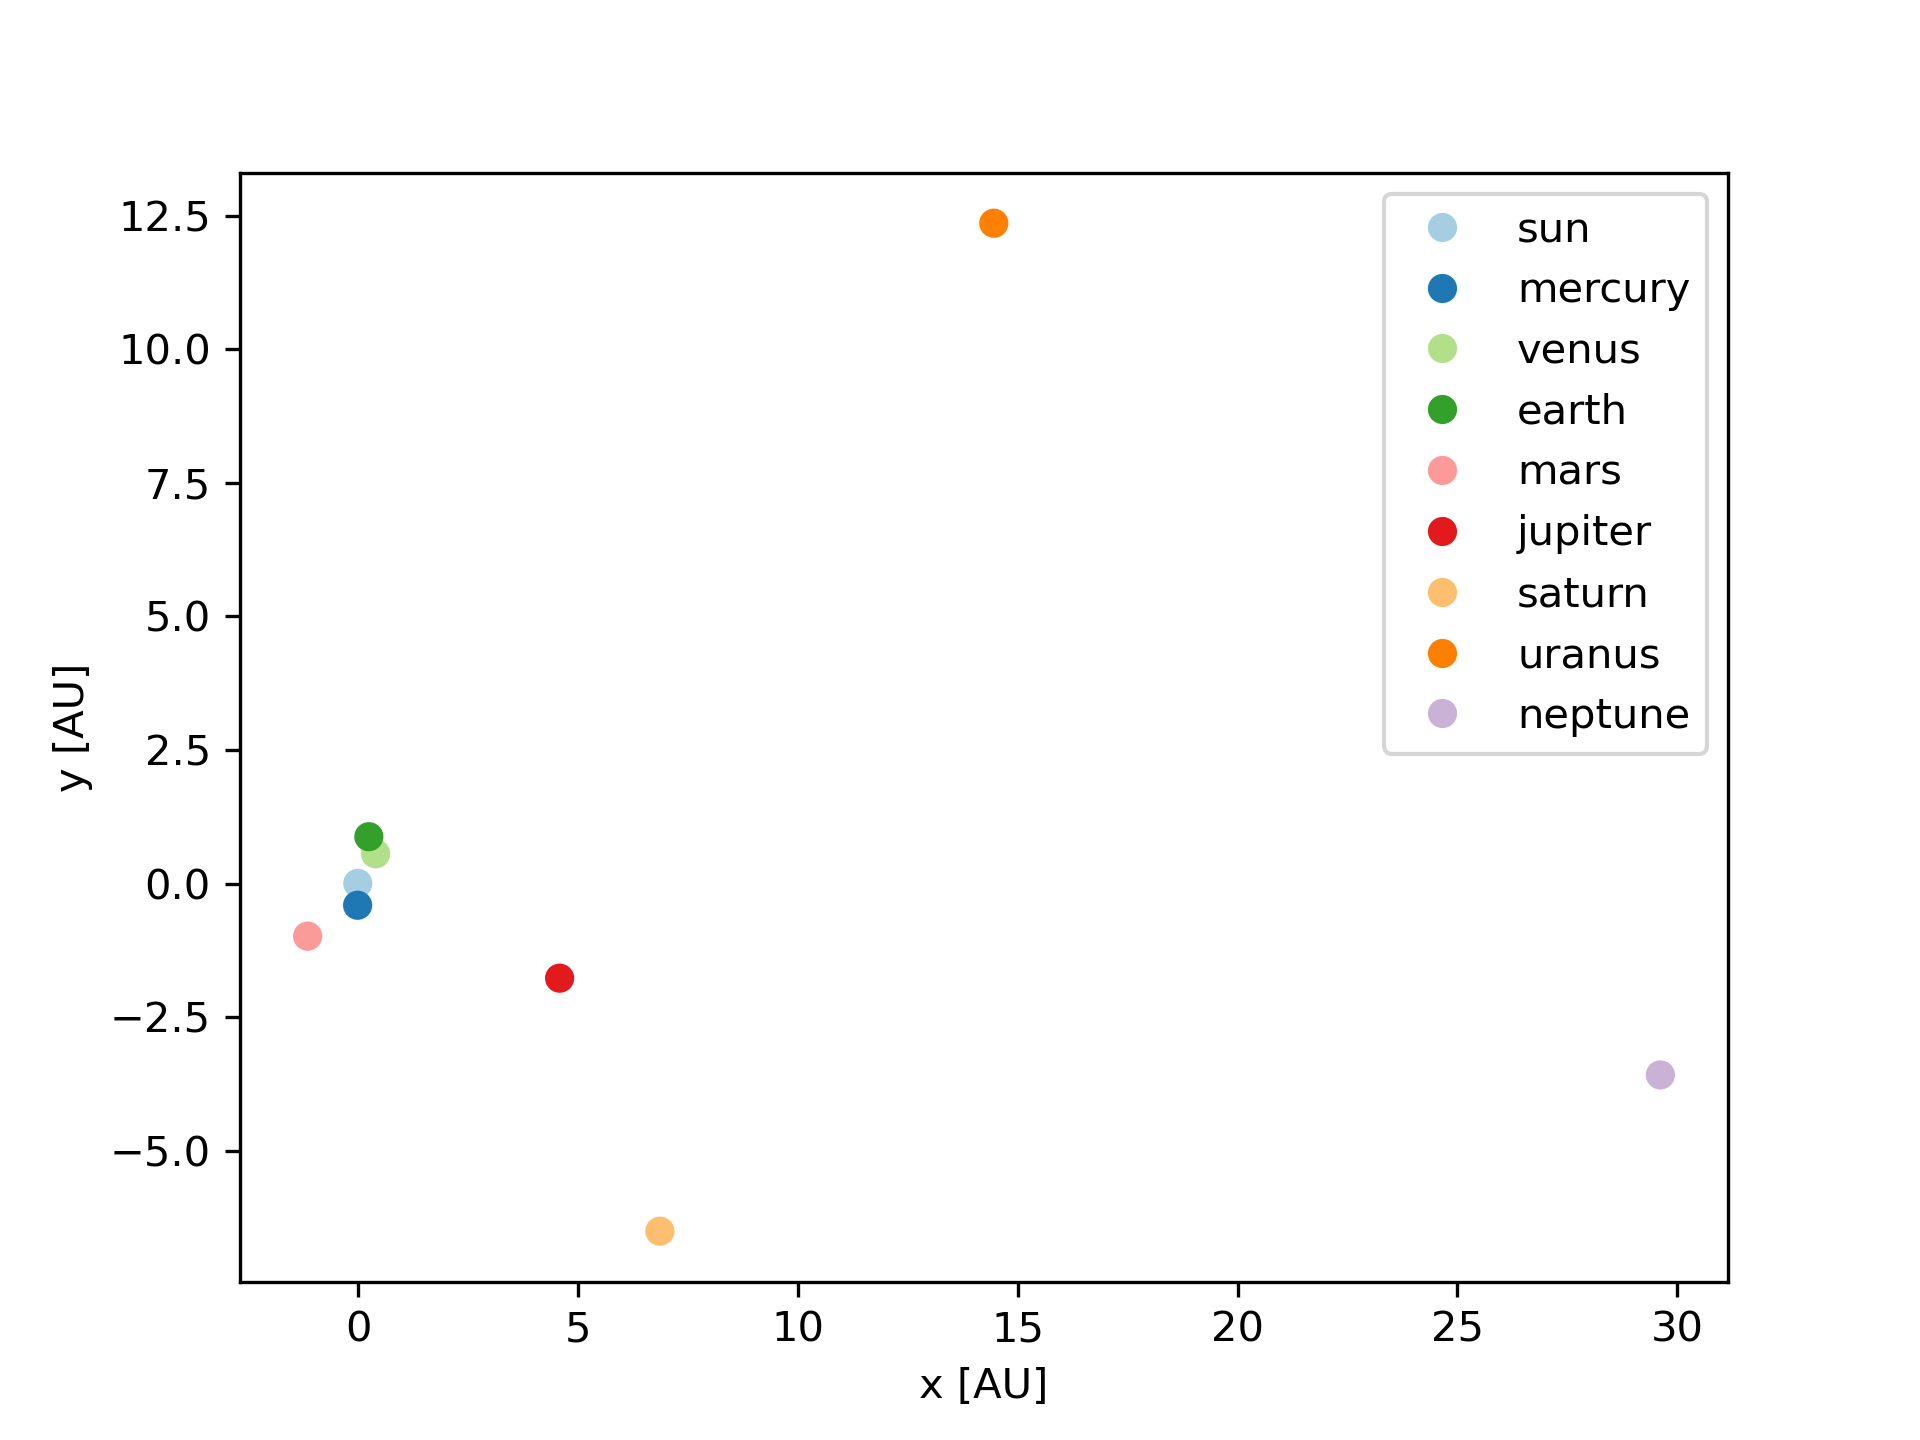
\includegraphics[width=.6\linewidth]{./plots/x-y.png}
  \caption{The initial x and y positions of all the 8 planets and the Sun.}
  \label{fig:x-y}
\end{figure}

\begin{figure}[H]
  \centering
  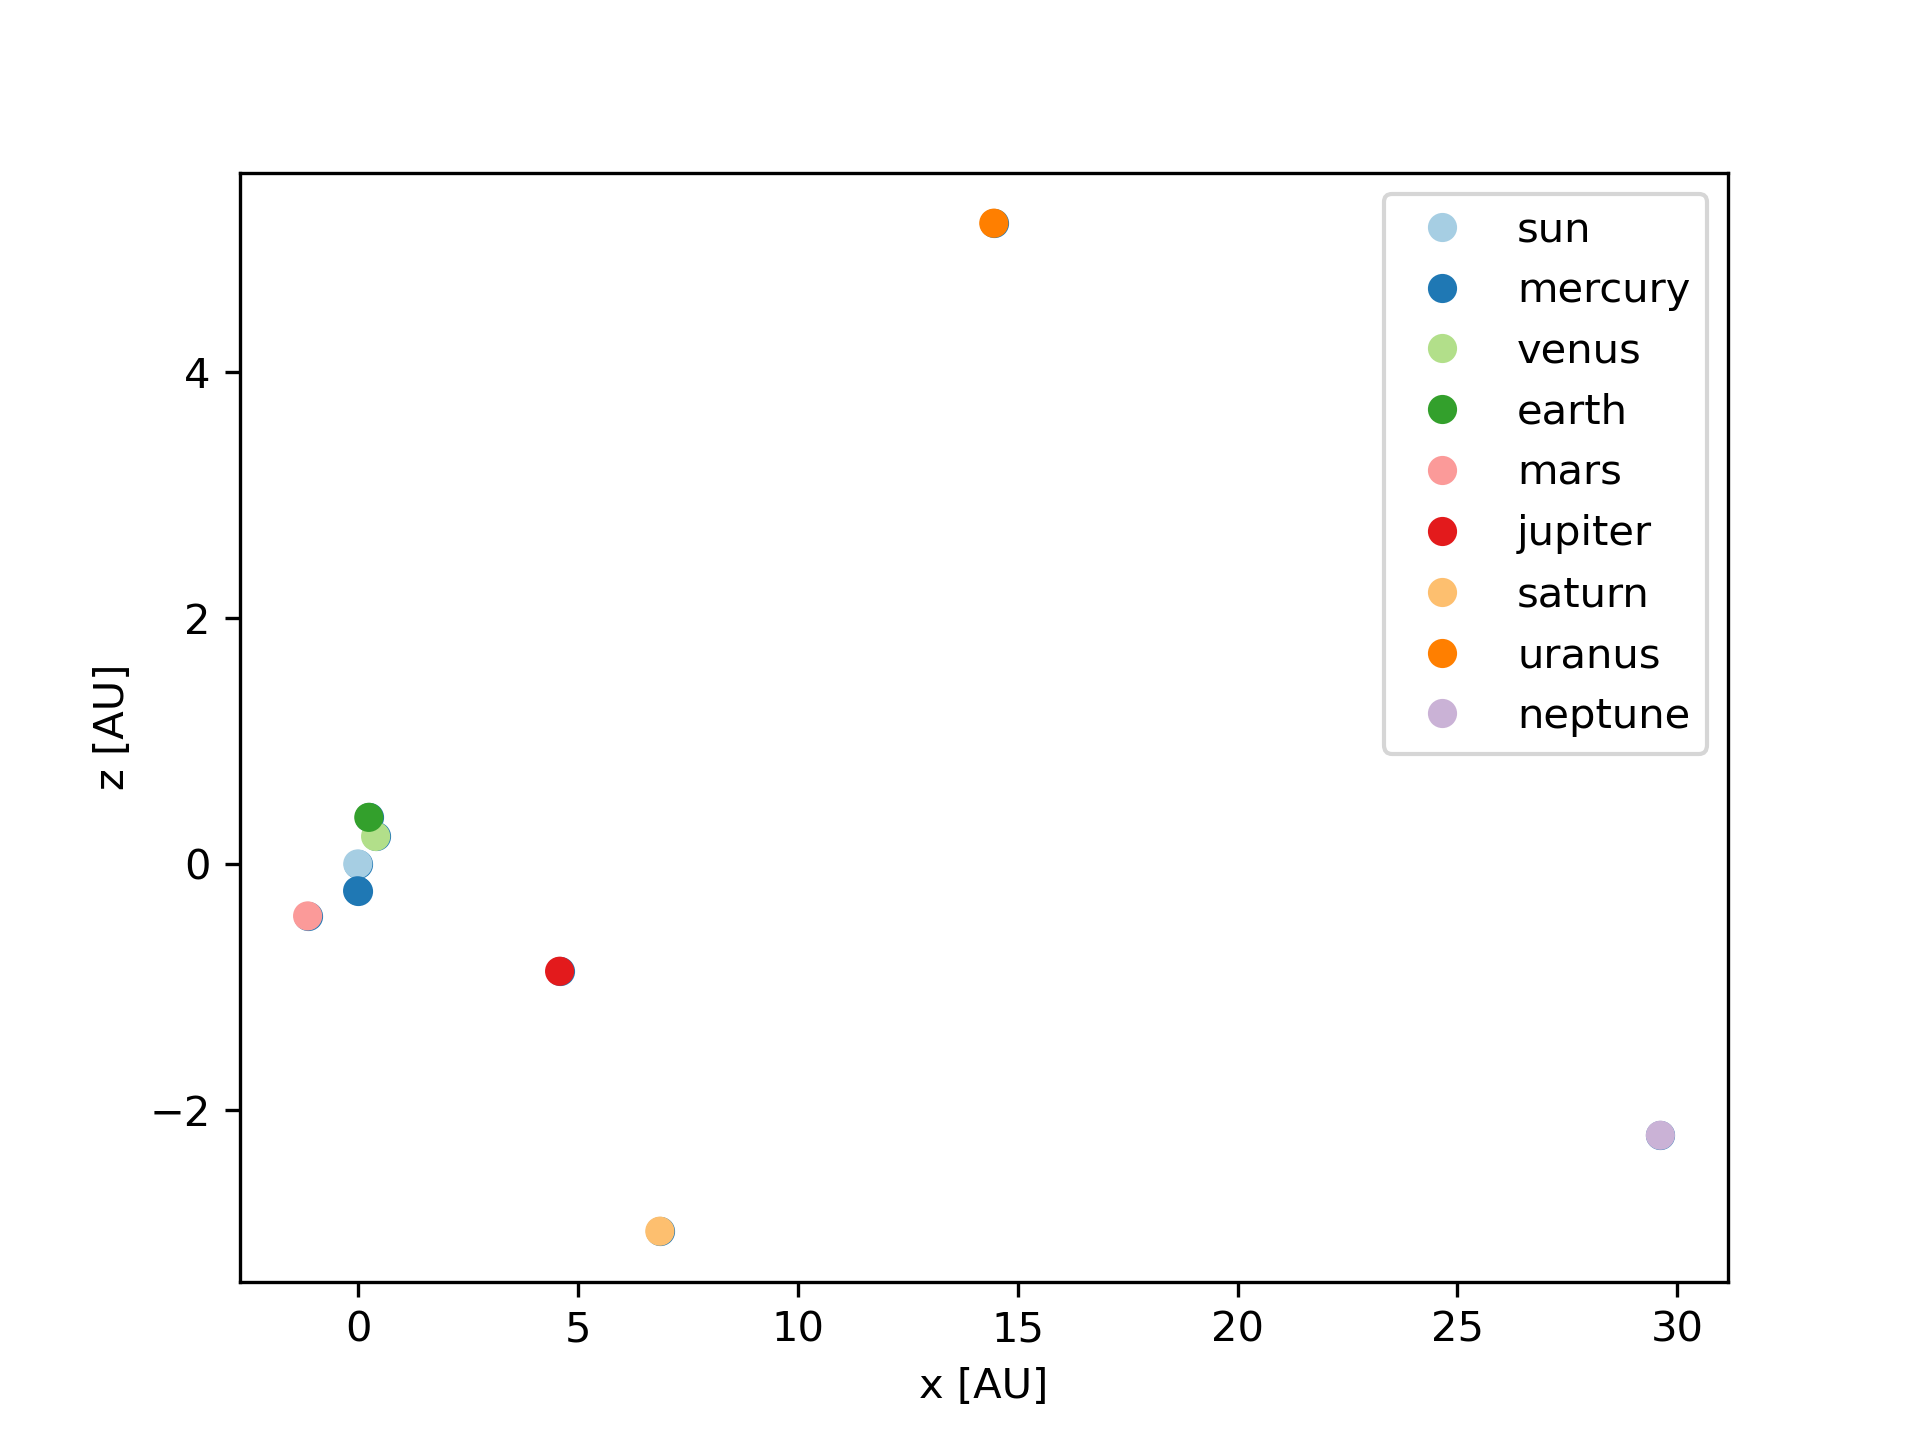
\includegraphics[width=.6\linewidth]{./plots/x-z.png}
  \caption{The initial x and z positions of all the 8 planets and the Sun.}
  \label{fig:x-z}
\end{figure}

\subsection{Solving with Leapfrog Algorithm}
\label{sec:leap}

We will now use the ``Leapfrog'' algorithm to integrate the differential equation for the gravitational forces. What we want to integrate is:
\begin{equation}
  r''(t) = - \frac{G M_{\odot}  r(t)}{|r(t)|^3}
\end{equation}
where $r(t)$ is the $(x,y,z)$ position of the planet and $r''(t)$ the acceleration. $G$ is the gravitational constant and $M_{\odot}$ is the mass of the Sun. We create the ``acceleration'' function for that use.

To solve this differential equation we implement the ``leapfrog'' function. We first initialize three arrays for $t,\;r,\;r'$, and then we solve using a loop calculating each time the position and velocity of the planet. We do that by kicking the planet at a half-step and then drifting the position of the planet accordingly. We then kick the planet at the other half-step. By doing that we make sure that there is symmetry when solving the 2nd-order differential equation. That ensures that our solutions are time-reversible and therefore energy is conserved. This makes Leapfrog a very suitable algorithm for solving orbital differential equations.

\lstinputlisting{leapfrog.py}

In the main part of the script we call the ``leapfrog'' function for all 8 planets and we give their initial positions and velocities. We want to solve it from the starting date and for 200 years with a step of 0.5 days. We then create plots for the evolution of the position of the planets on the x-y plane and also plot the evolution of the z-position of the planets. We can find those plots in \Cref{fig:xy-leap,fig:xy-leap-zoom,fig:z-leap,fig:z-leap-zoom}. As we can see the solutions are correct since all our planets rotate around the sun with stability over the course of the 200 years. Only Mercury shows some instability, the orbit is however close and does not diverge. For the evolution of the z positions, we can find the expected sinusoidal lines, with higher periods and amplitudes for the planets that are further away from the sun. This is also what we expect since the period of these lines should be the rotational period of each planet and the amplitude represents how far from the ecliptic plane can each planet get, which is higher for planets further away from the sun. 

\begin{figure}[H]
  \centering
  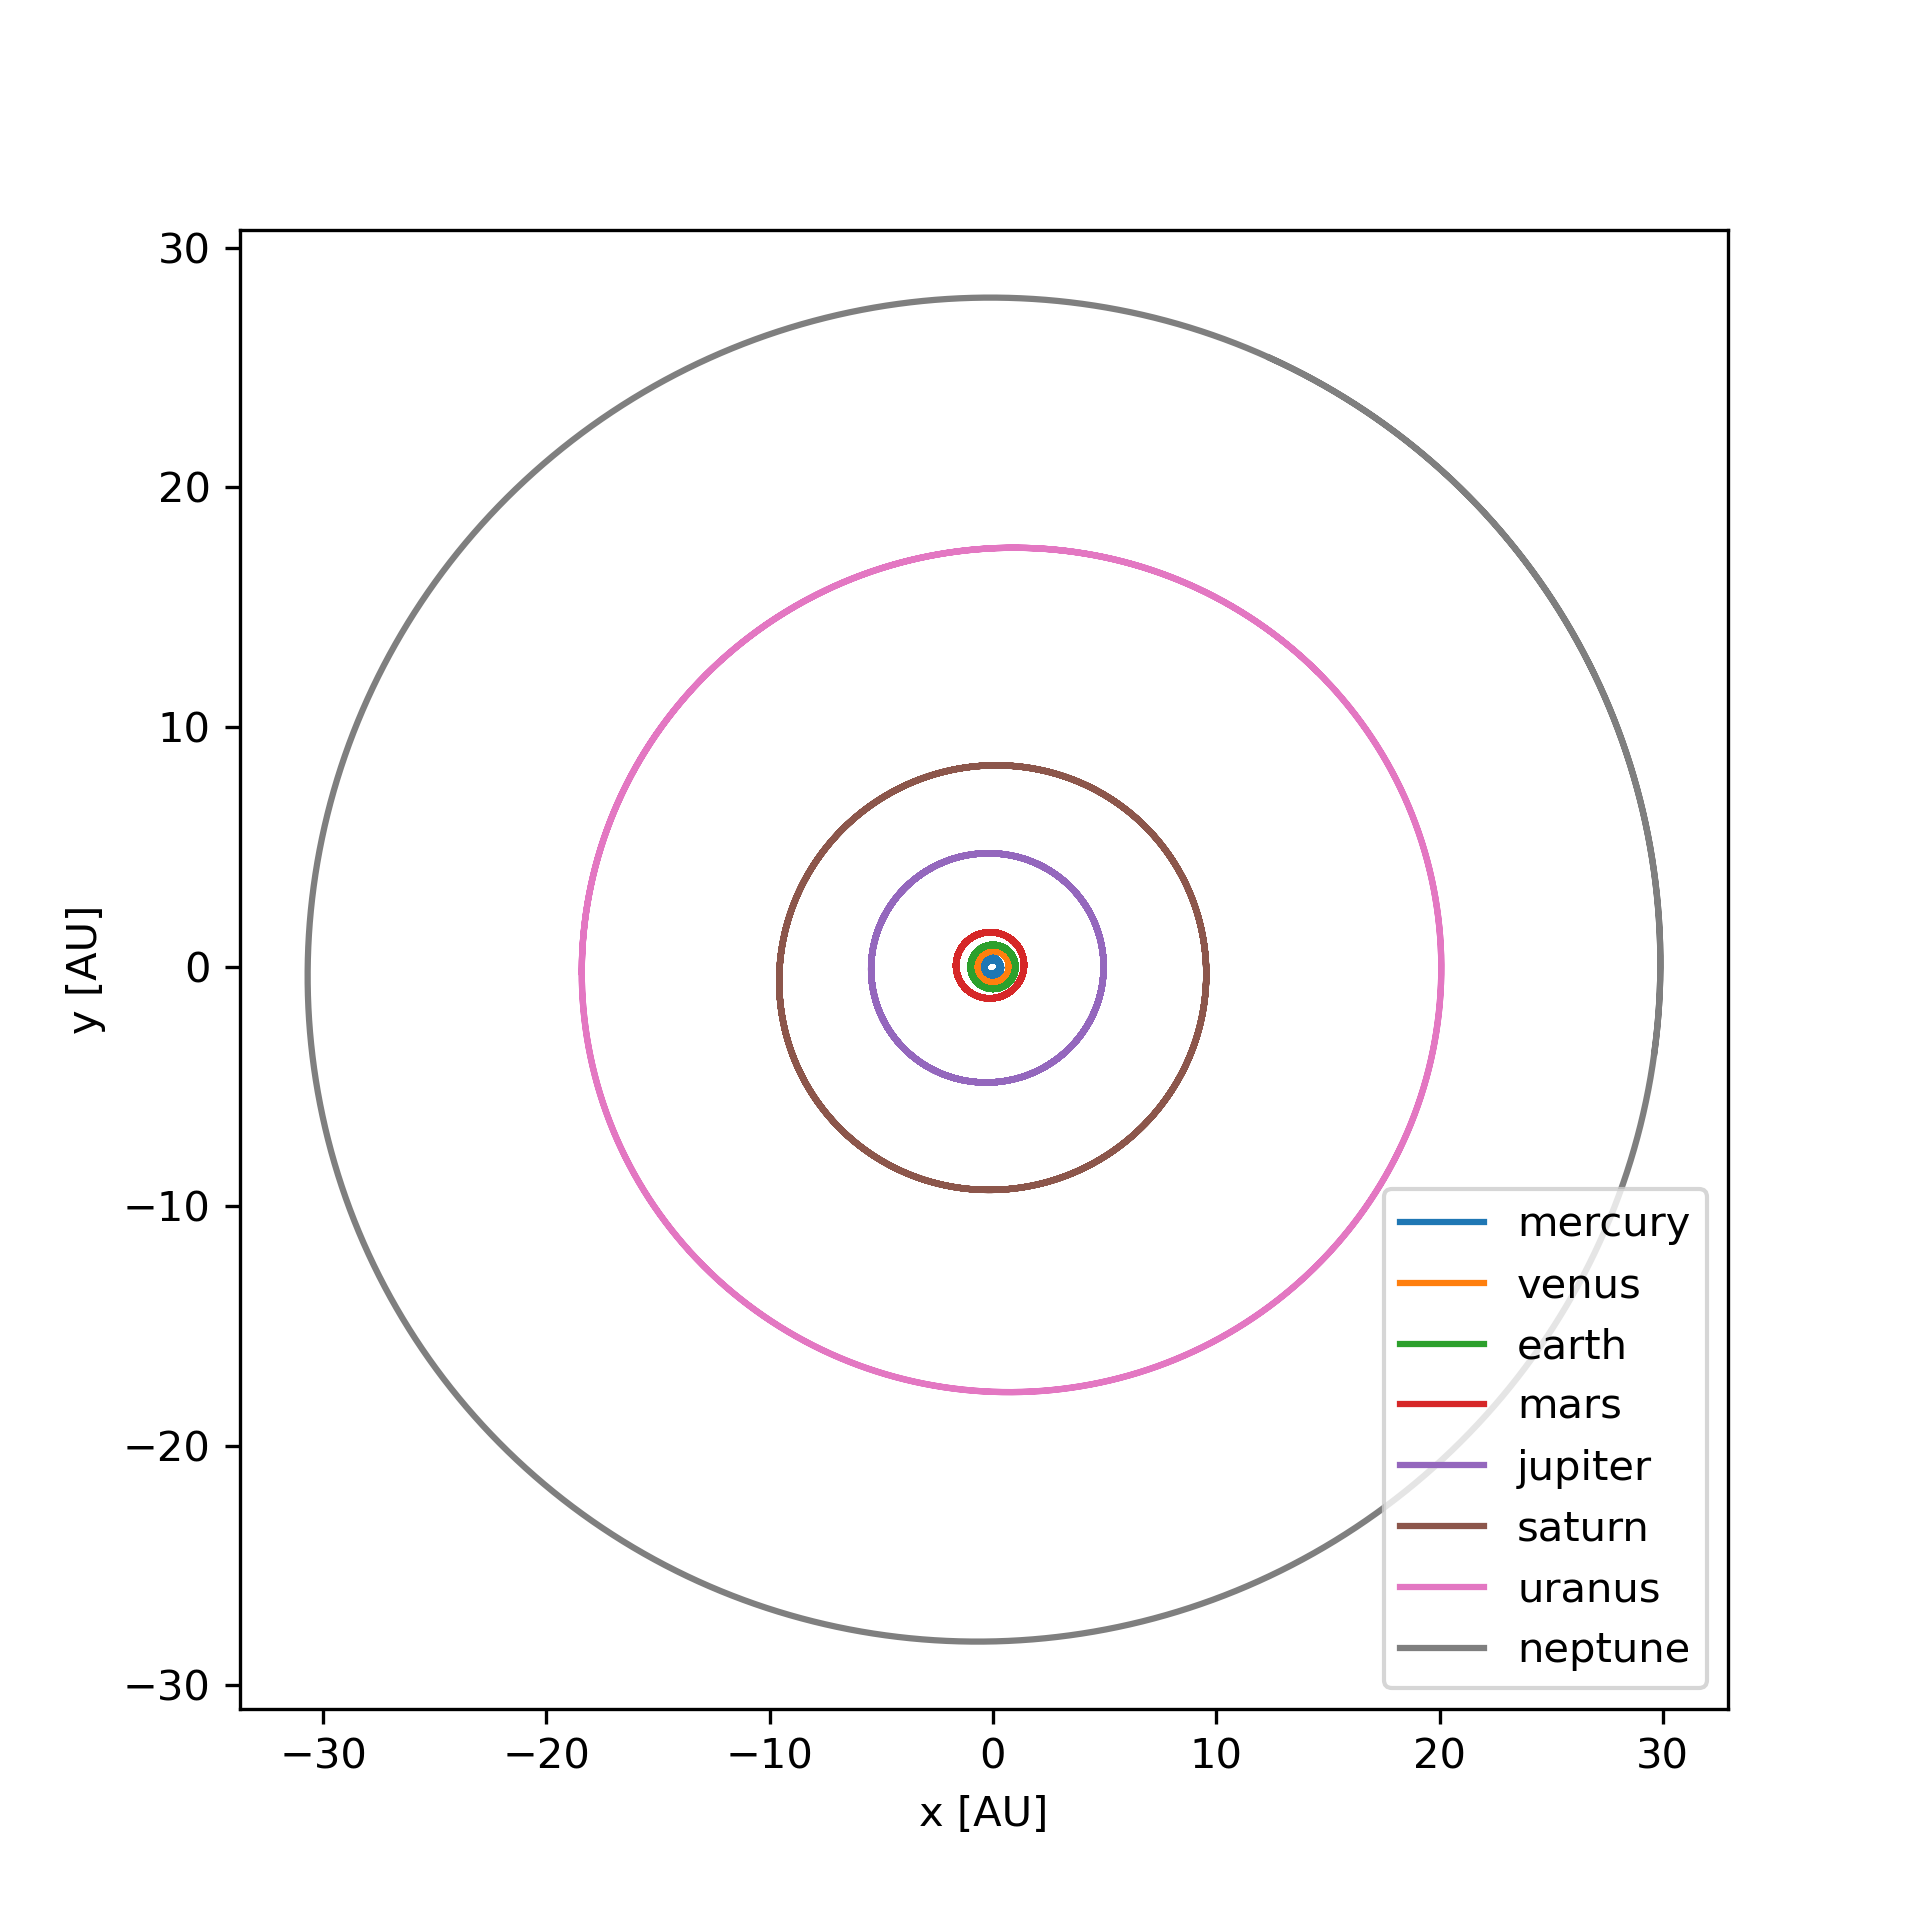
\includegraphics[width=.60\linewidth]{./plots/xy-leapfrog.png}
  \caption{The evolution of the x and y positions of all the 8 planets when integrating using the Leapfrog algorithm.}
  \label{fig:xy-leap}
\end{figure}

\begin{figure}[H]
  \centering
  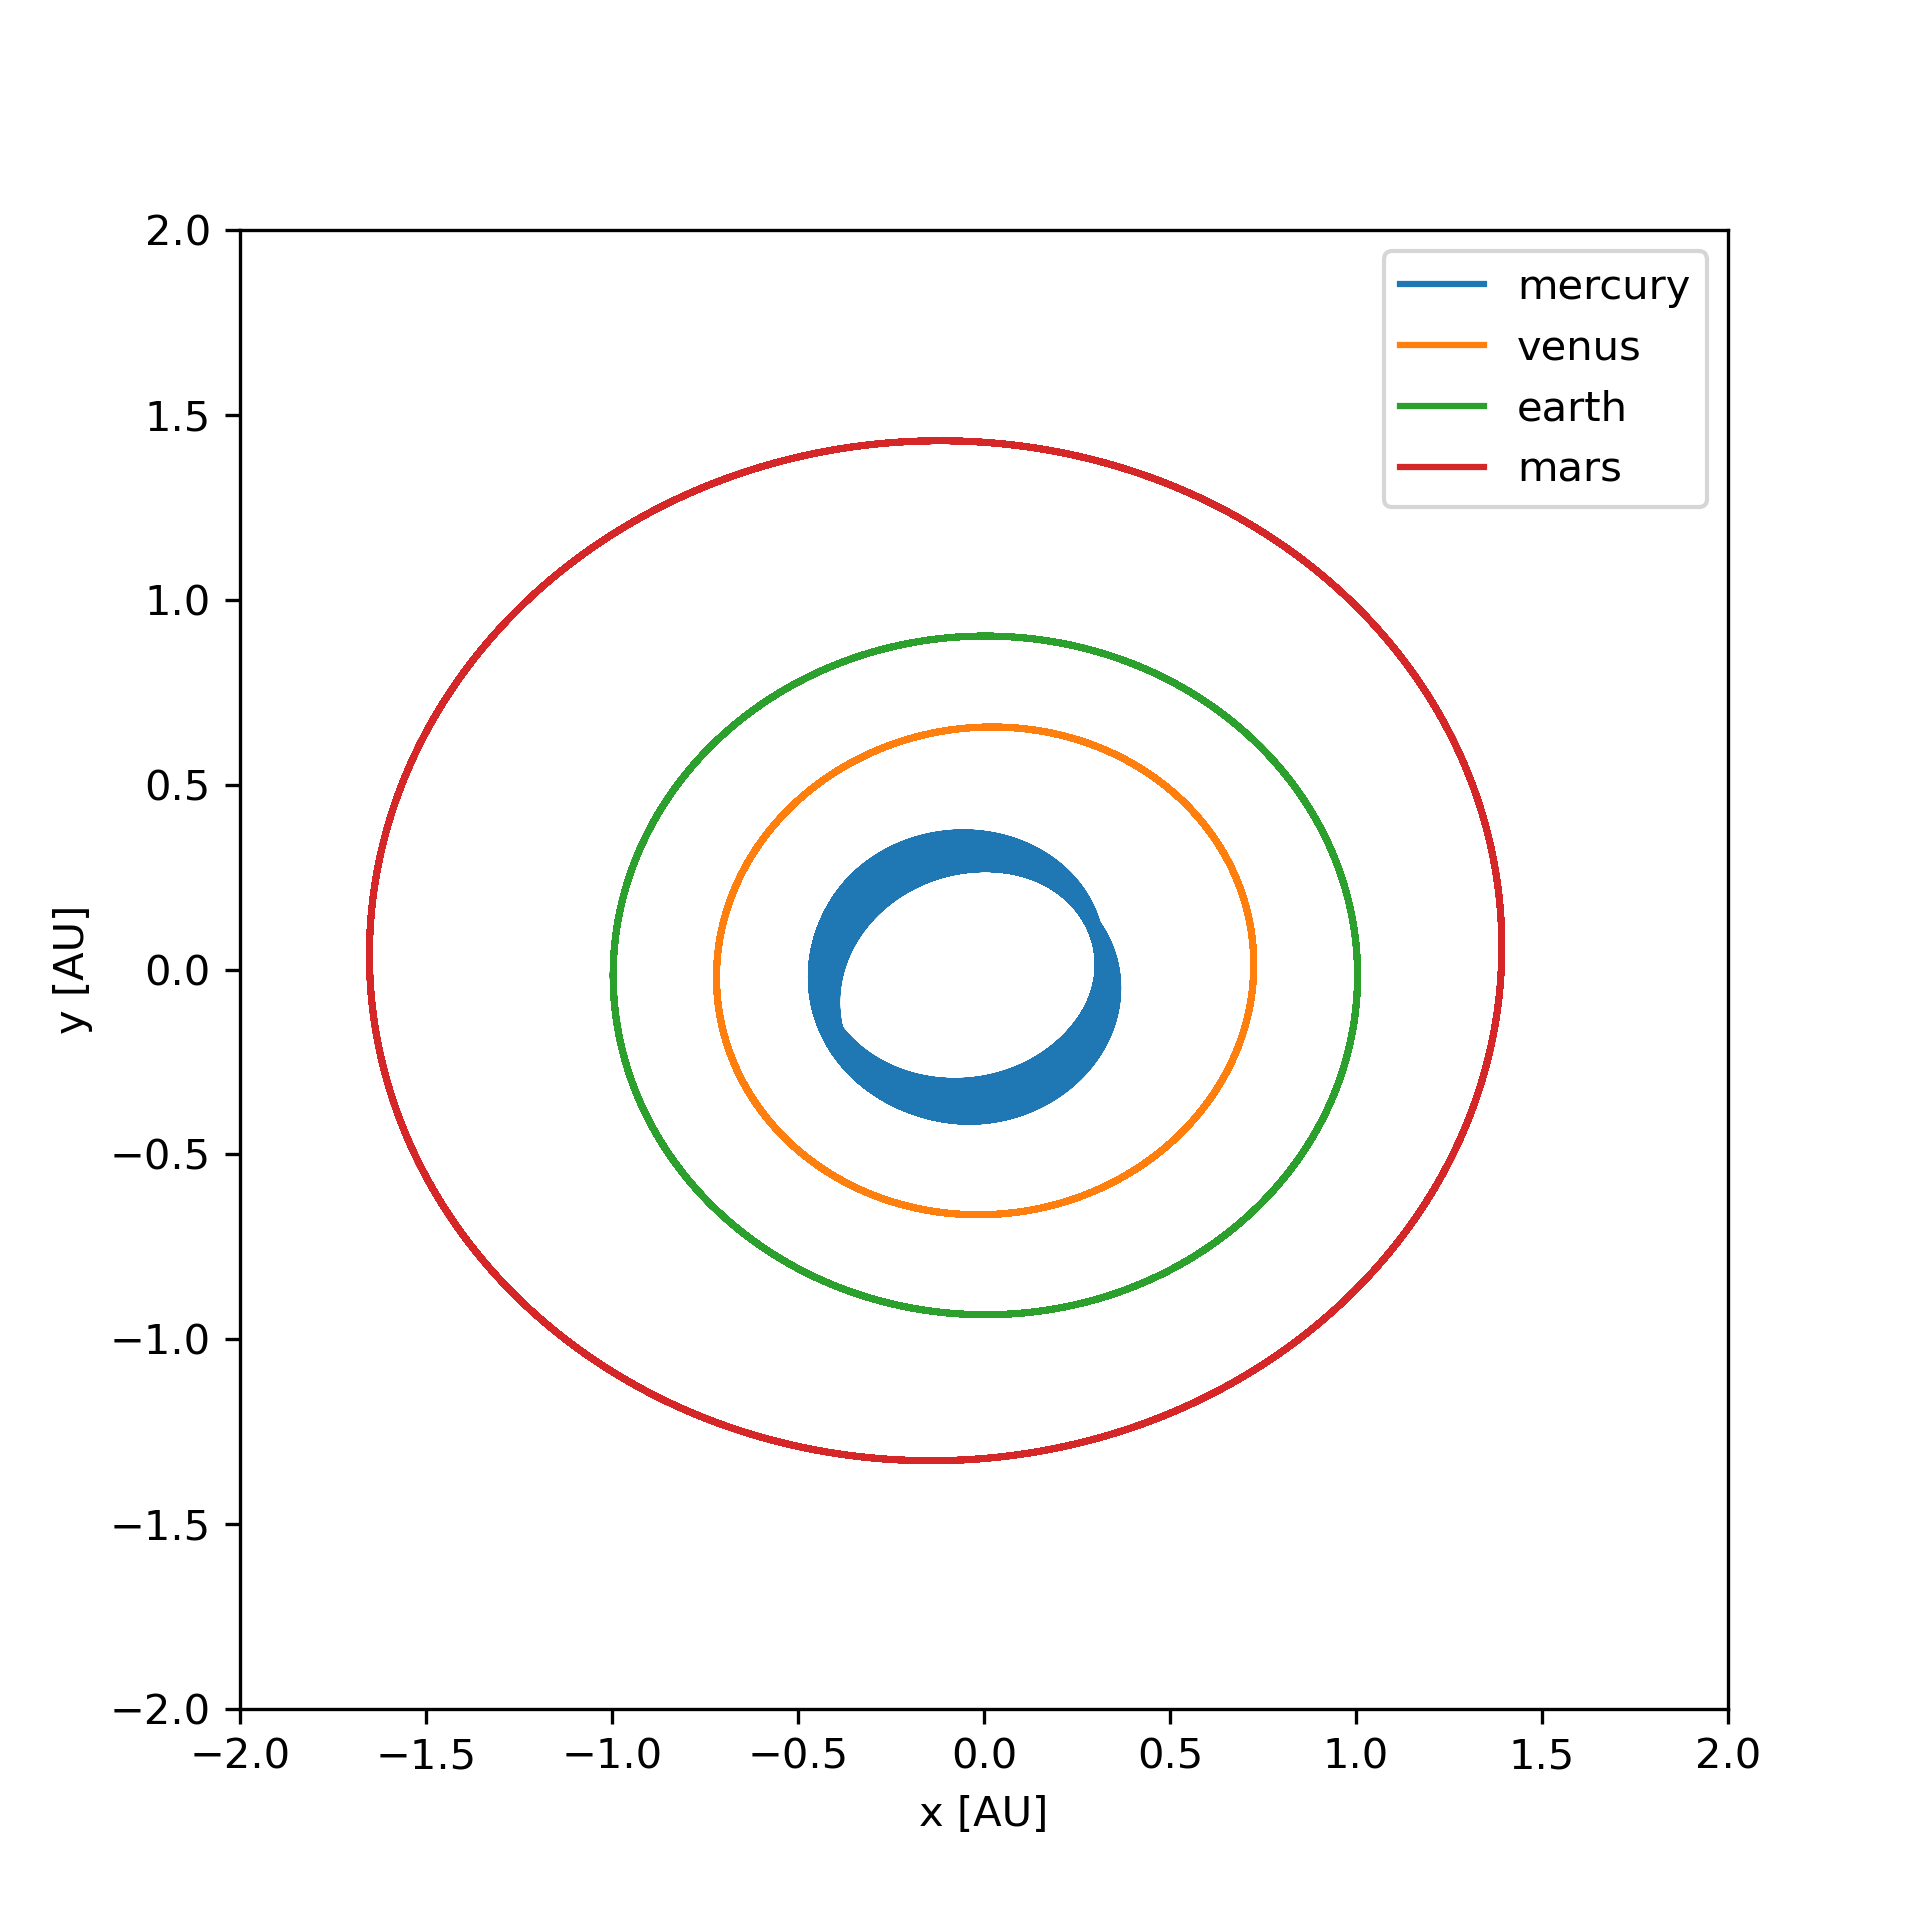
\includegraphics[width=.60\linewidth]{./plots/xy-leapfrog-zoom.png}
  \caption{The evolution of the x and y positions of the 4 inner planets when integrating using the Leapfrog algorithm.}
  \label{fig:xy-leap-zoom}
\end{figure}

\begin{figure}[H]
  \centering
  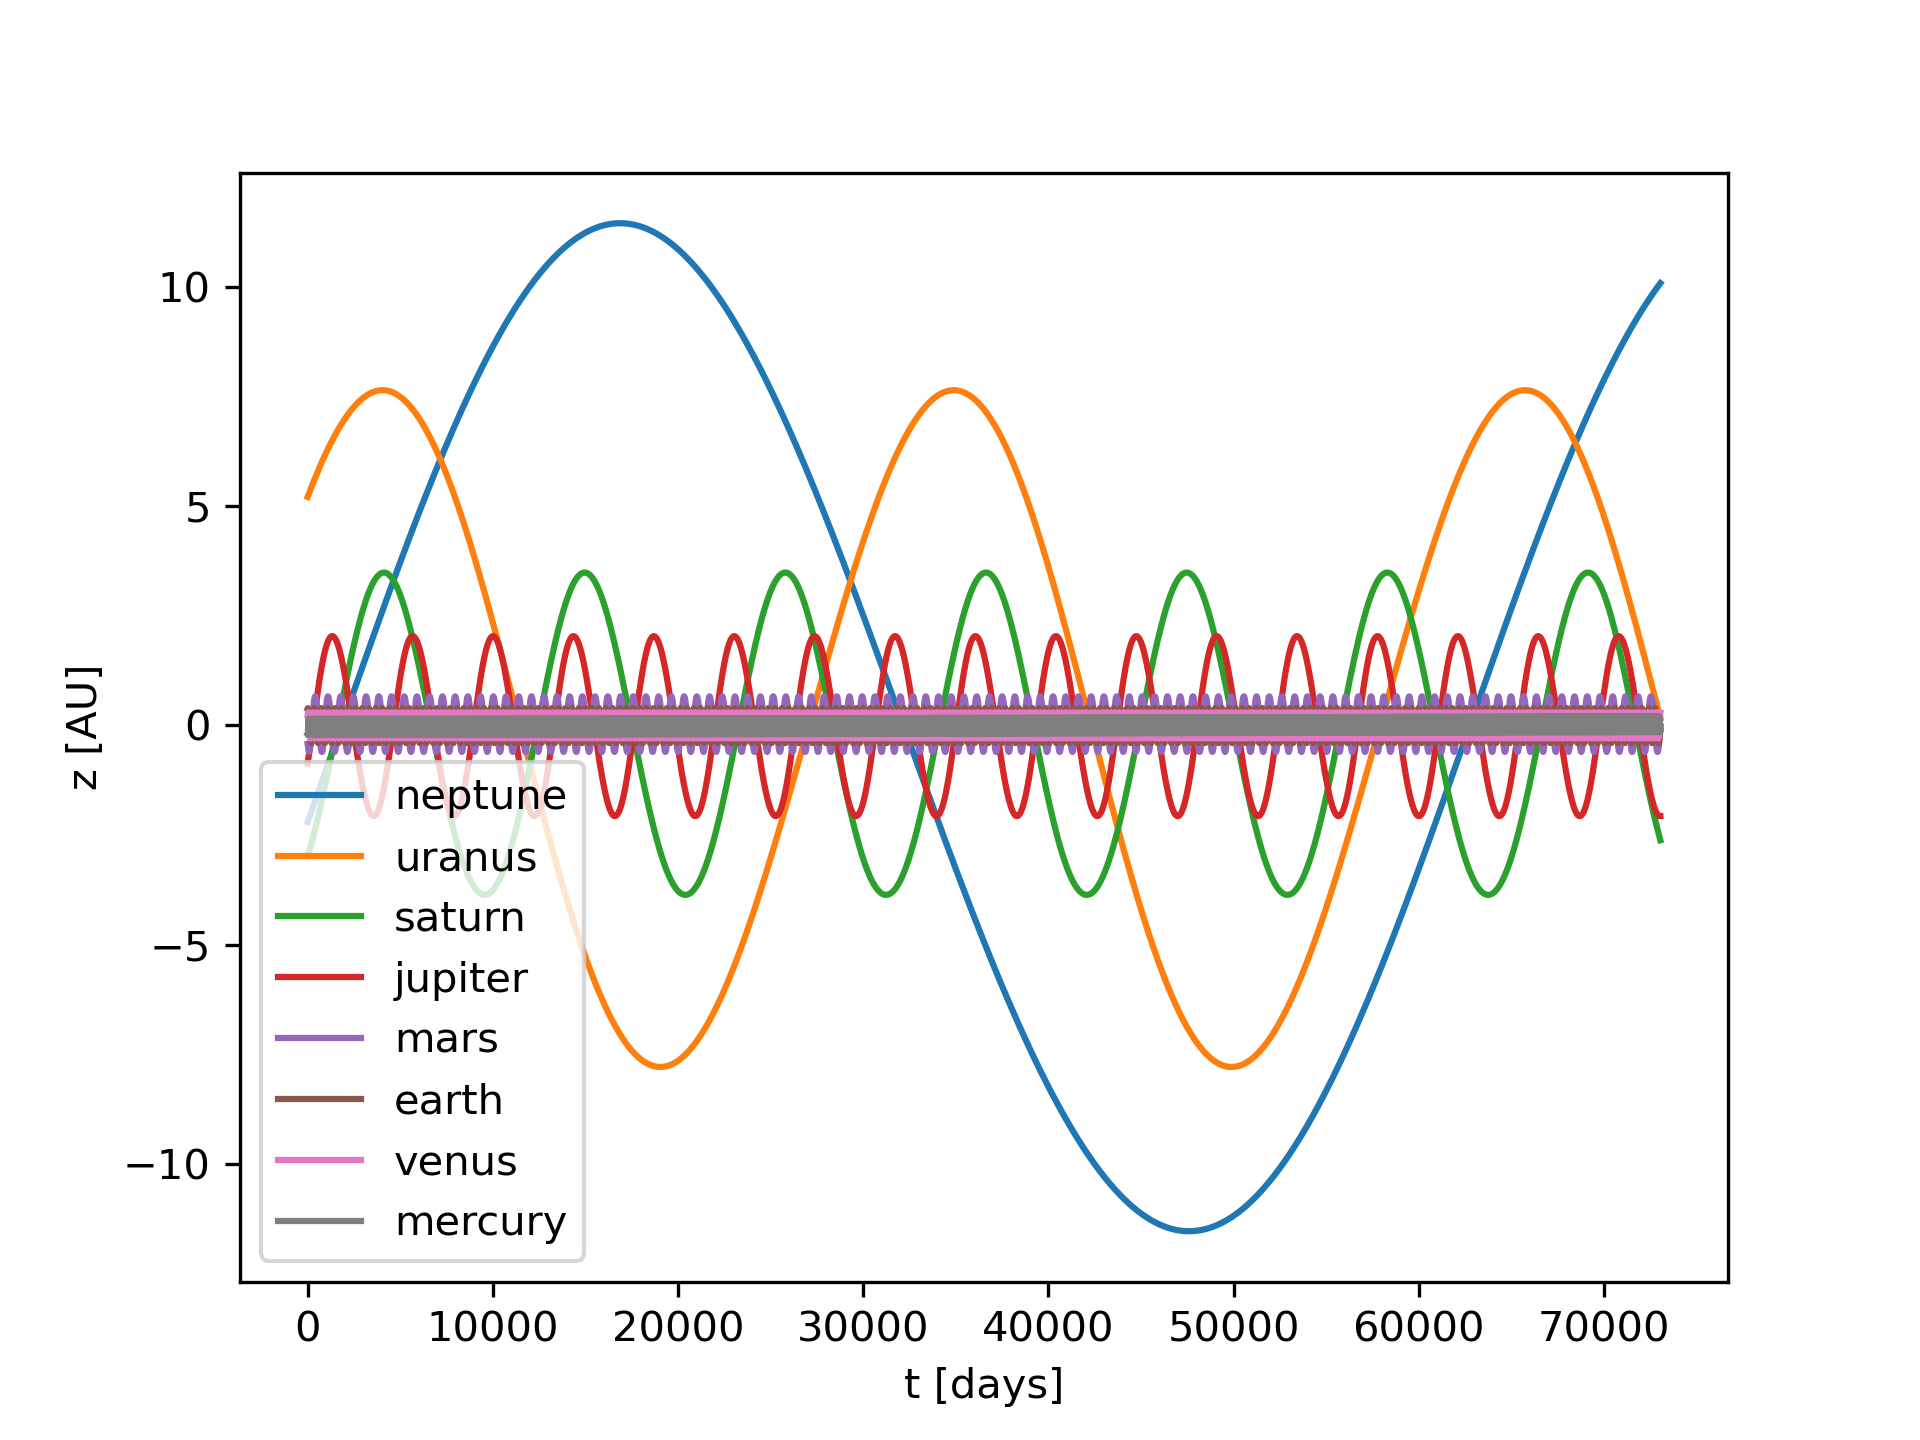
\includegraphics[width=.8\linewidth]{./plots/z-leapfrog.png}
  \caption{The evolution of the z positions of all the 8 planets when integrating using the Leapfrog algorithm.}
  \label{fig:z-leap}
\end{figure}

\begin{figure}[H]
  \centering
  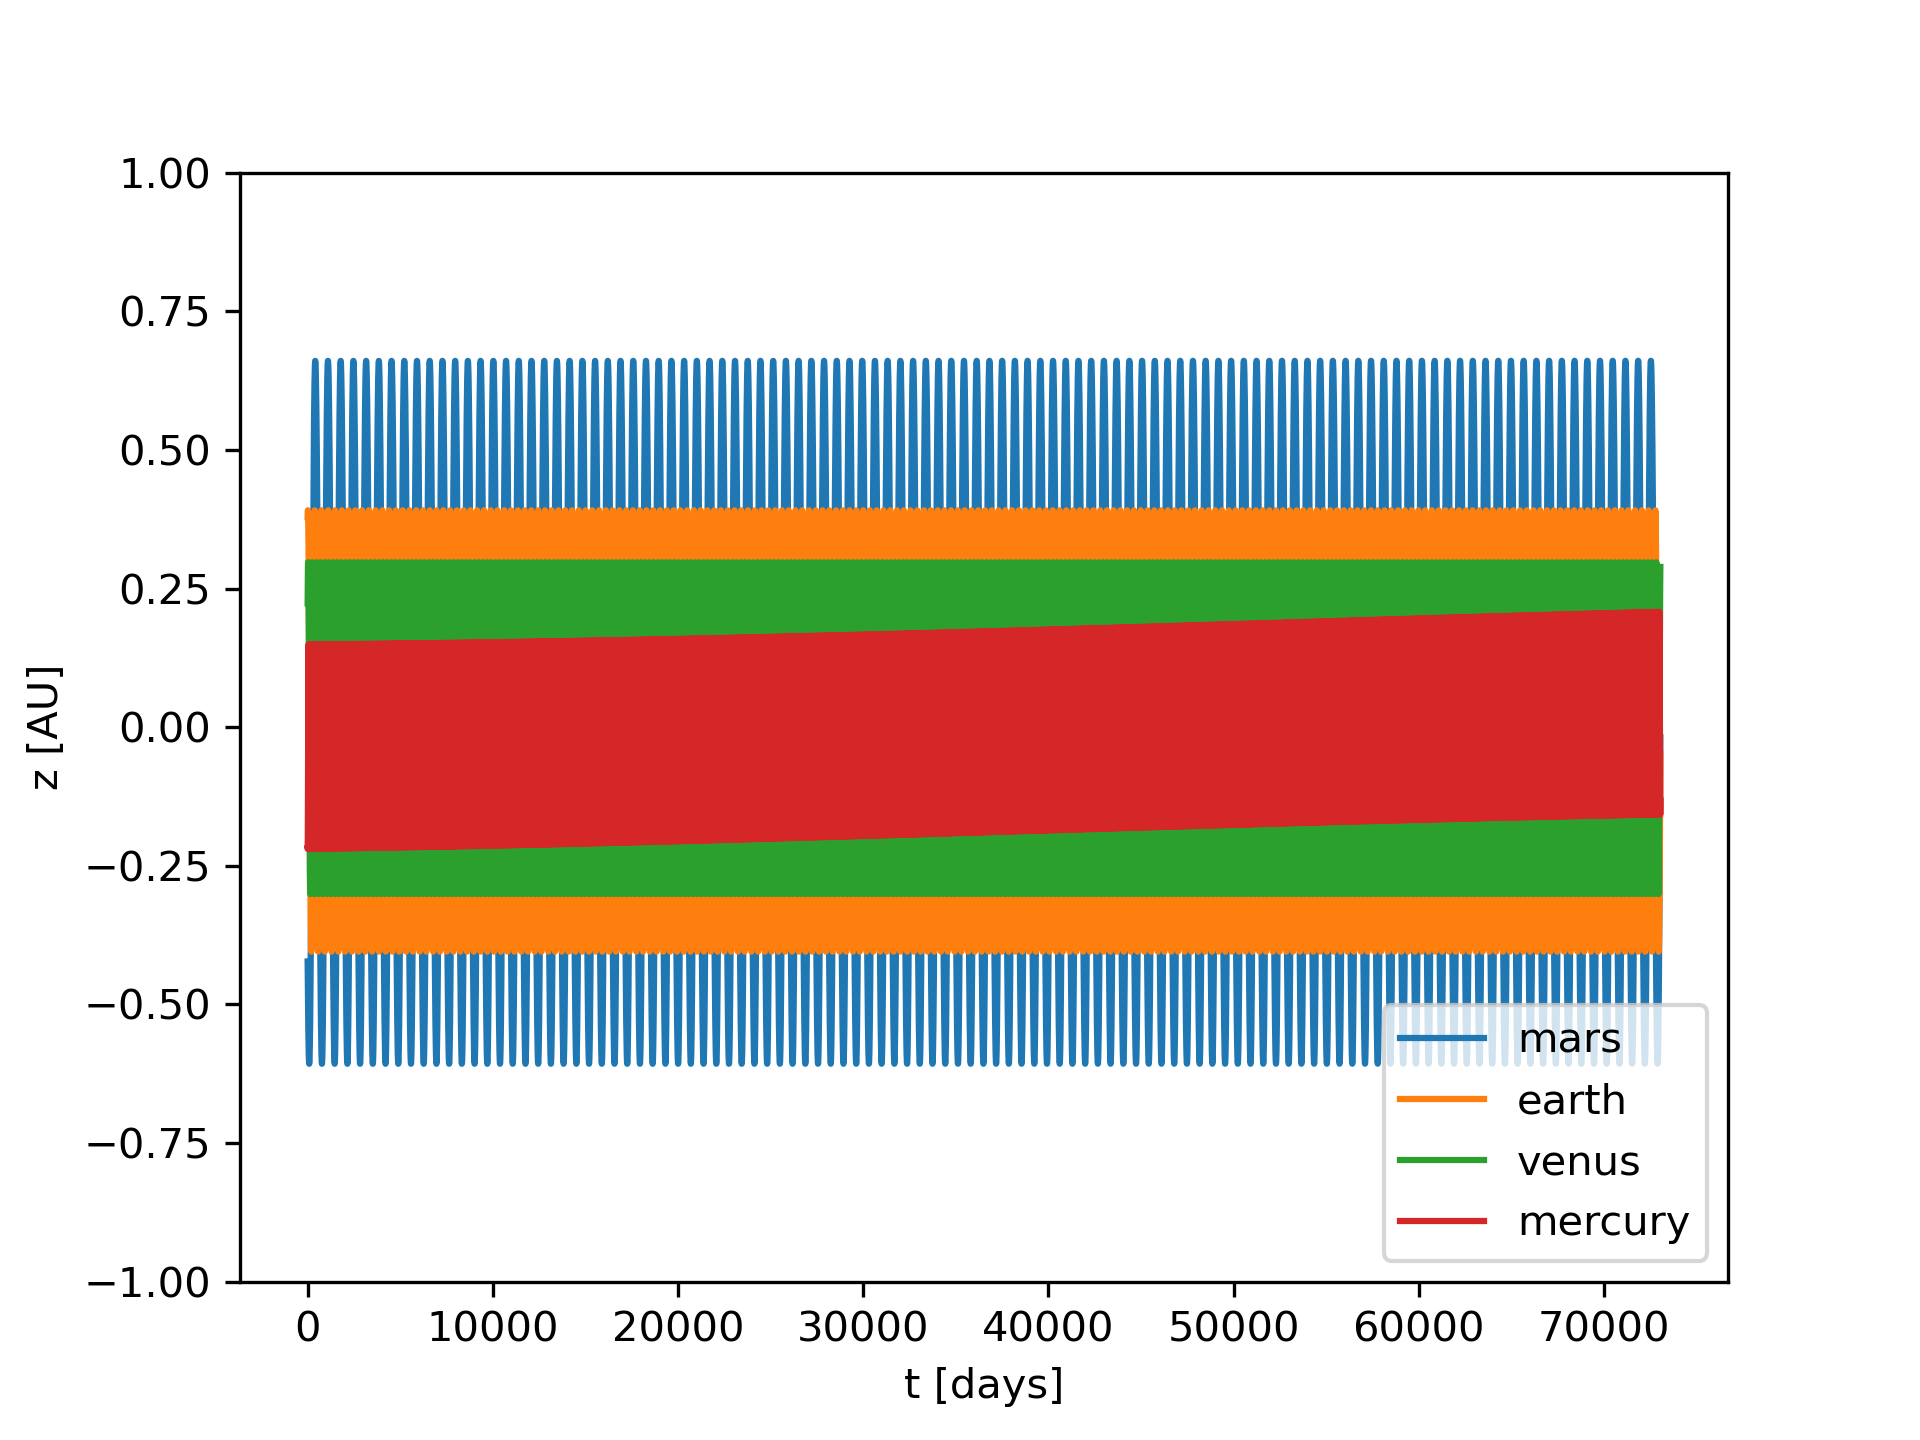
\includegraphics[width=.8\linewidth]{./plots/z-leapfrog-zoom.png}
  \caption{The evolution of the z positions of the 4 inner planets when integrating using the Leapfrog algorithm.}
  \label{fig:z-leap-zoom}
\end{figure}

\subsection{Solving with Euler's Algorithm}

We also want to solve the system using Euler's algorithm. For this, we implement the ``euler'' function which utilizes this algorithm to solve the 2nd-order differential equation. We once again initialize three arrays for $t,\;r,\;r'$ and then solve using a loop and the appropriate equations for Euler's algorithm. We also need to import all the initial conditions from the previous script with the function for the differential equation. 

\lstinputlisting{euler.py}

In the main part of the code, we solve the orbits of all 8 planets using our function. We then create the same plots we did in \Cref{sec:leap} to compare the new implementation with the previous one. As we can see in \Cref{fig:xy-eul,fig:xy-eul-zoom,fig:z-eul,fig:z-eul-zoom} the Euler's algorithm managed to solve the orbits there is however the issue of divergence. This is more evident for the planets closer to the Sun which makes sense as they have a smaller orbital period and they therefore achieve more full rotations around the Sun in our simulation time. This divergence can be seen in \Cref{fig:xy-eul} as the orbits of the inner planets, and especially mercury, get bigger. It also becomes more clear when looking at the orbits of the inner planets in \Cref{fig:xy-eul-zoom}. In \Cref{fig:z-eul} the amplitudes of the sinusoidal lines of the inner planets get greater as time progresses. In \Cref{fig:z-eul-zoom} the divergence becomes more clear as we see the z evolution of the inner planets. We also plot the difference in x positions between the Leapfrog and Euler's algorithm in \Cref{fig:x-leap-eul}. We can see how the divergence affected all the planets. The outer planets got affected less and due to their big orbital radius the difference could not be seen in the previous plots. 

\begin{figure}[H]
  \centering
  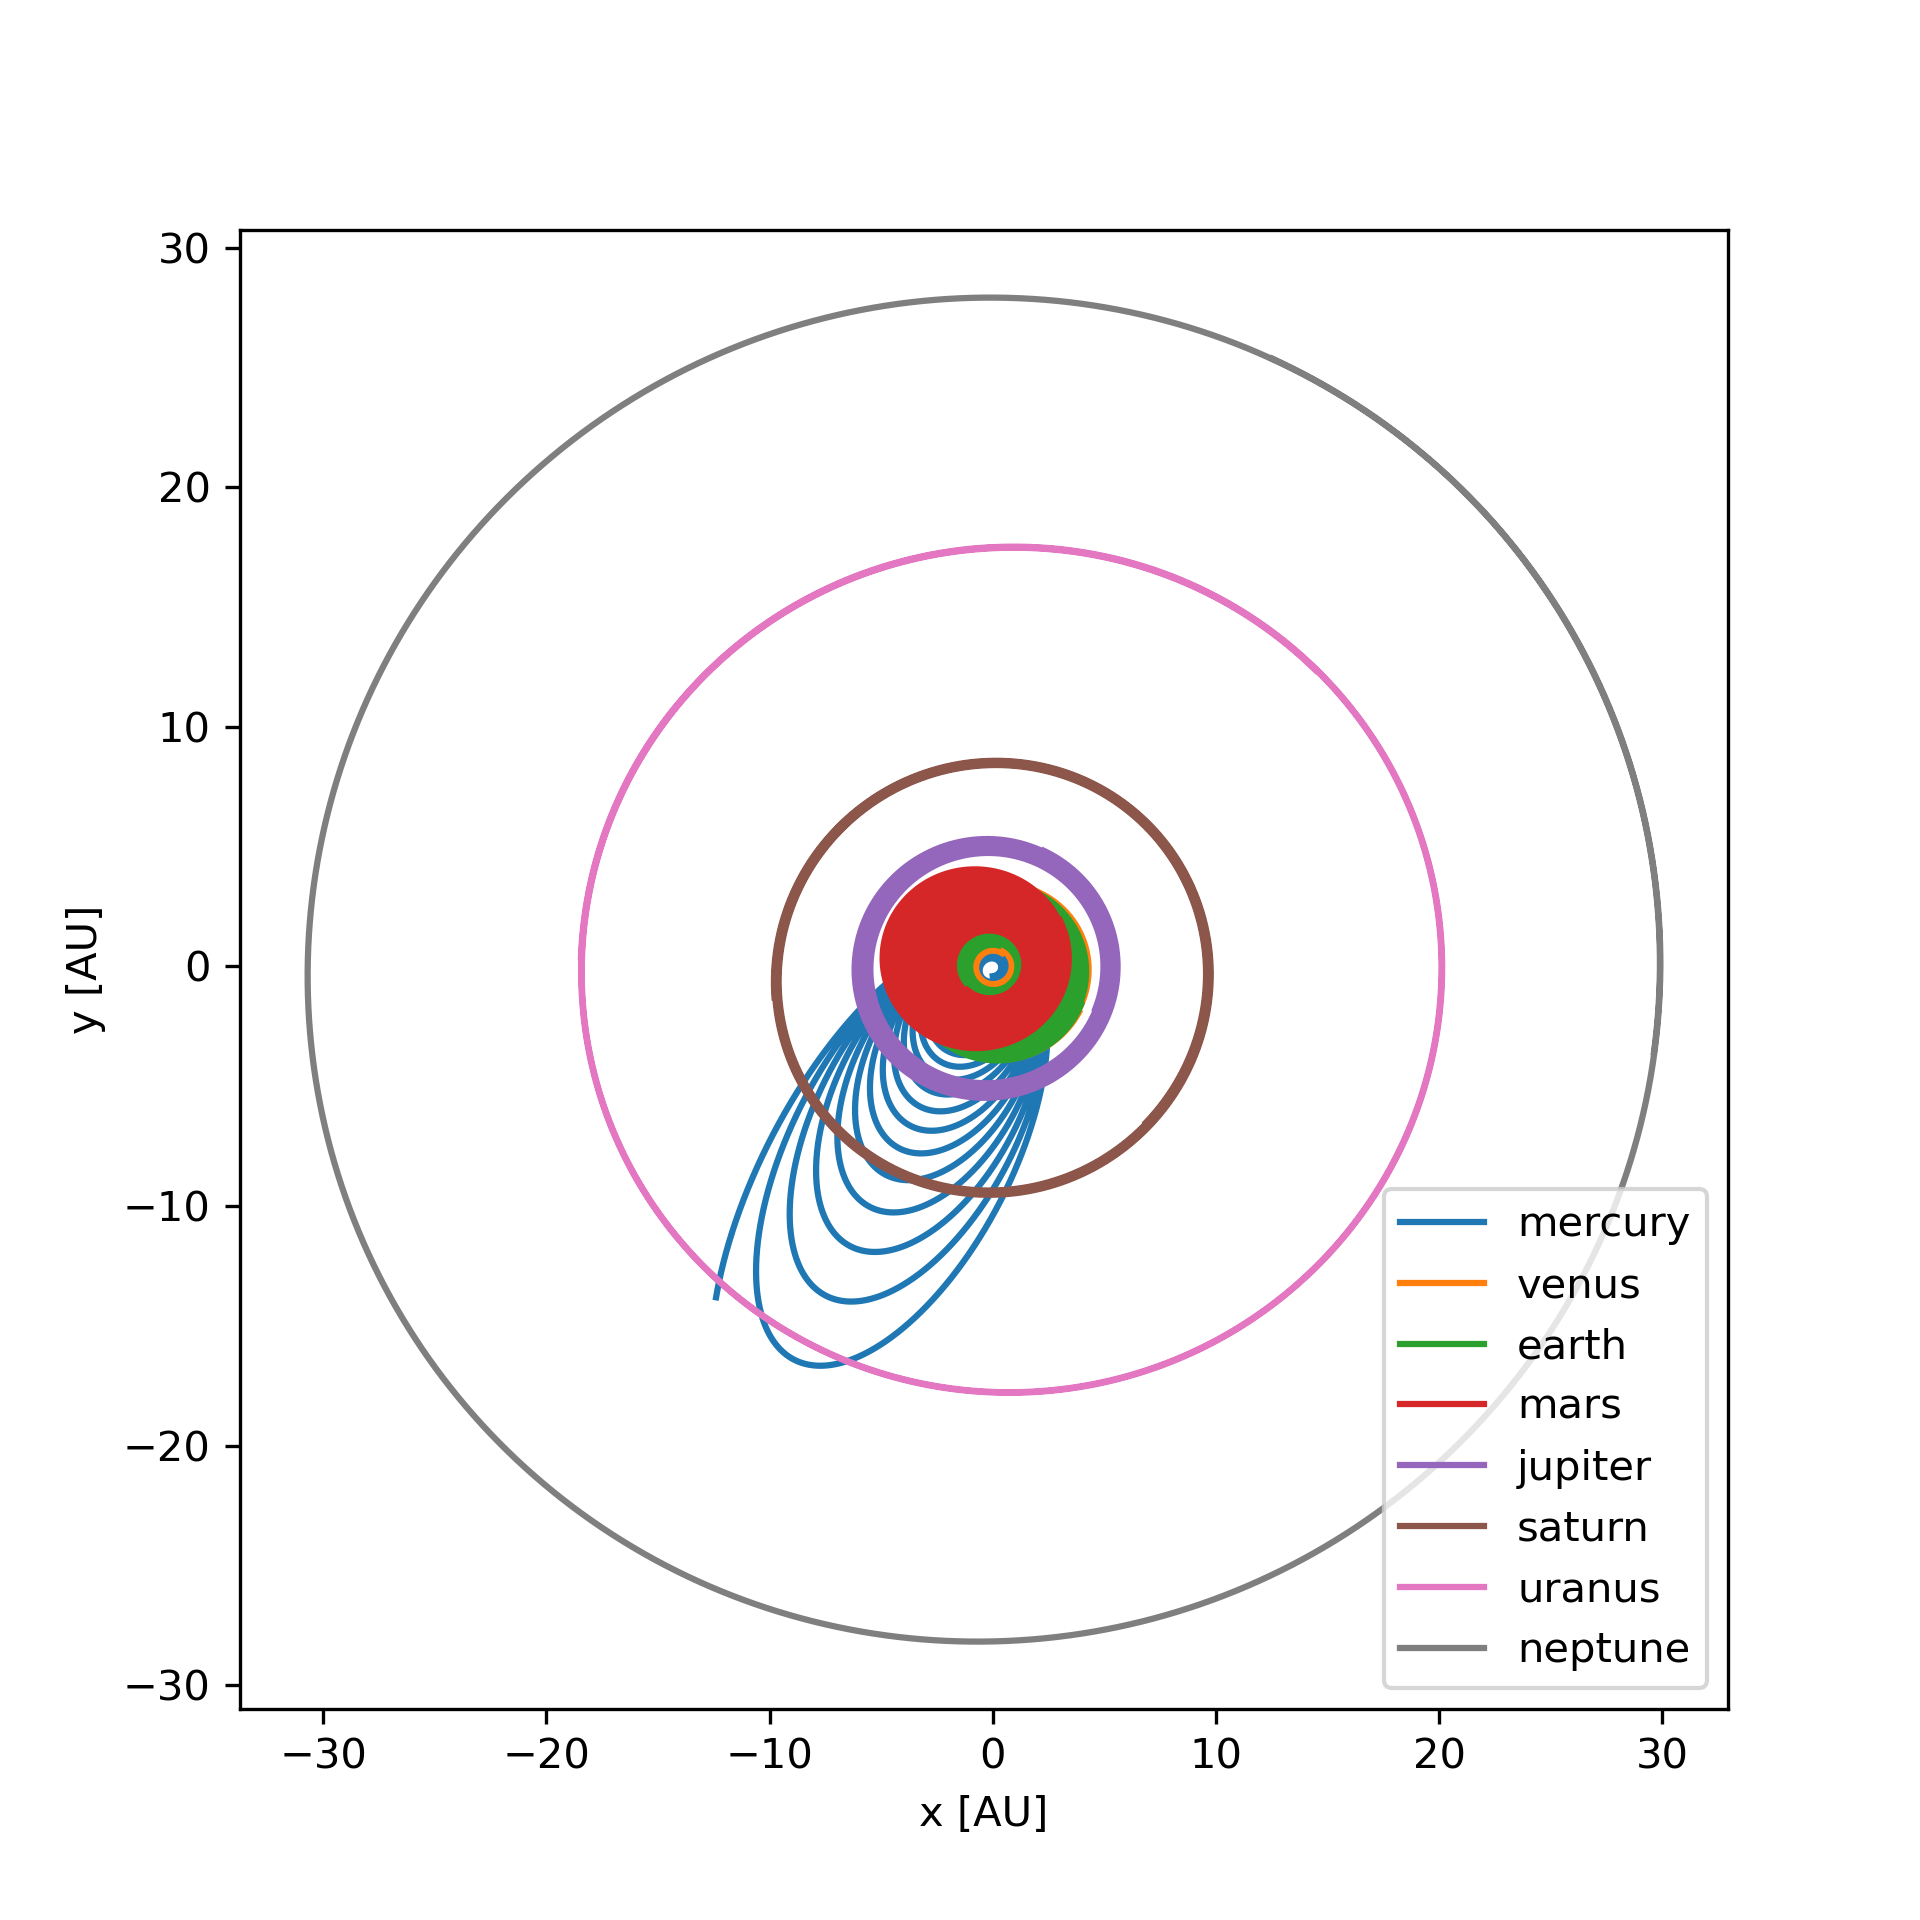
\includegraphics[width=.60\linewidth]{./plots/xy-euler.png}
  \caption{The evolution of the x and y positions of all the 8 planets when integrating using Euler's algorithm. We can see the divergence of the inner planets.}
  \label{fig:xy-eul}
\end{figure}

\begin{figure}[H]
  \centering
  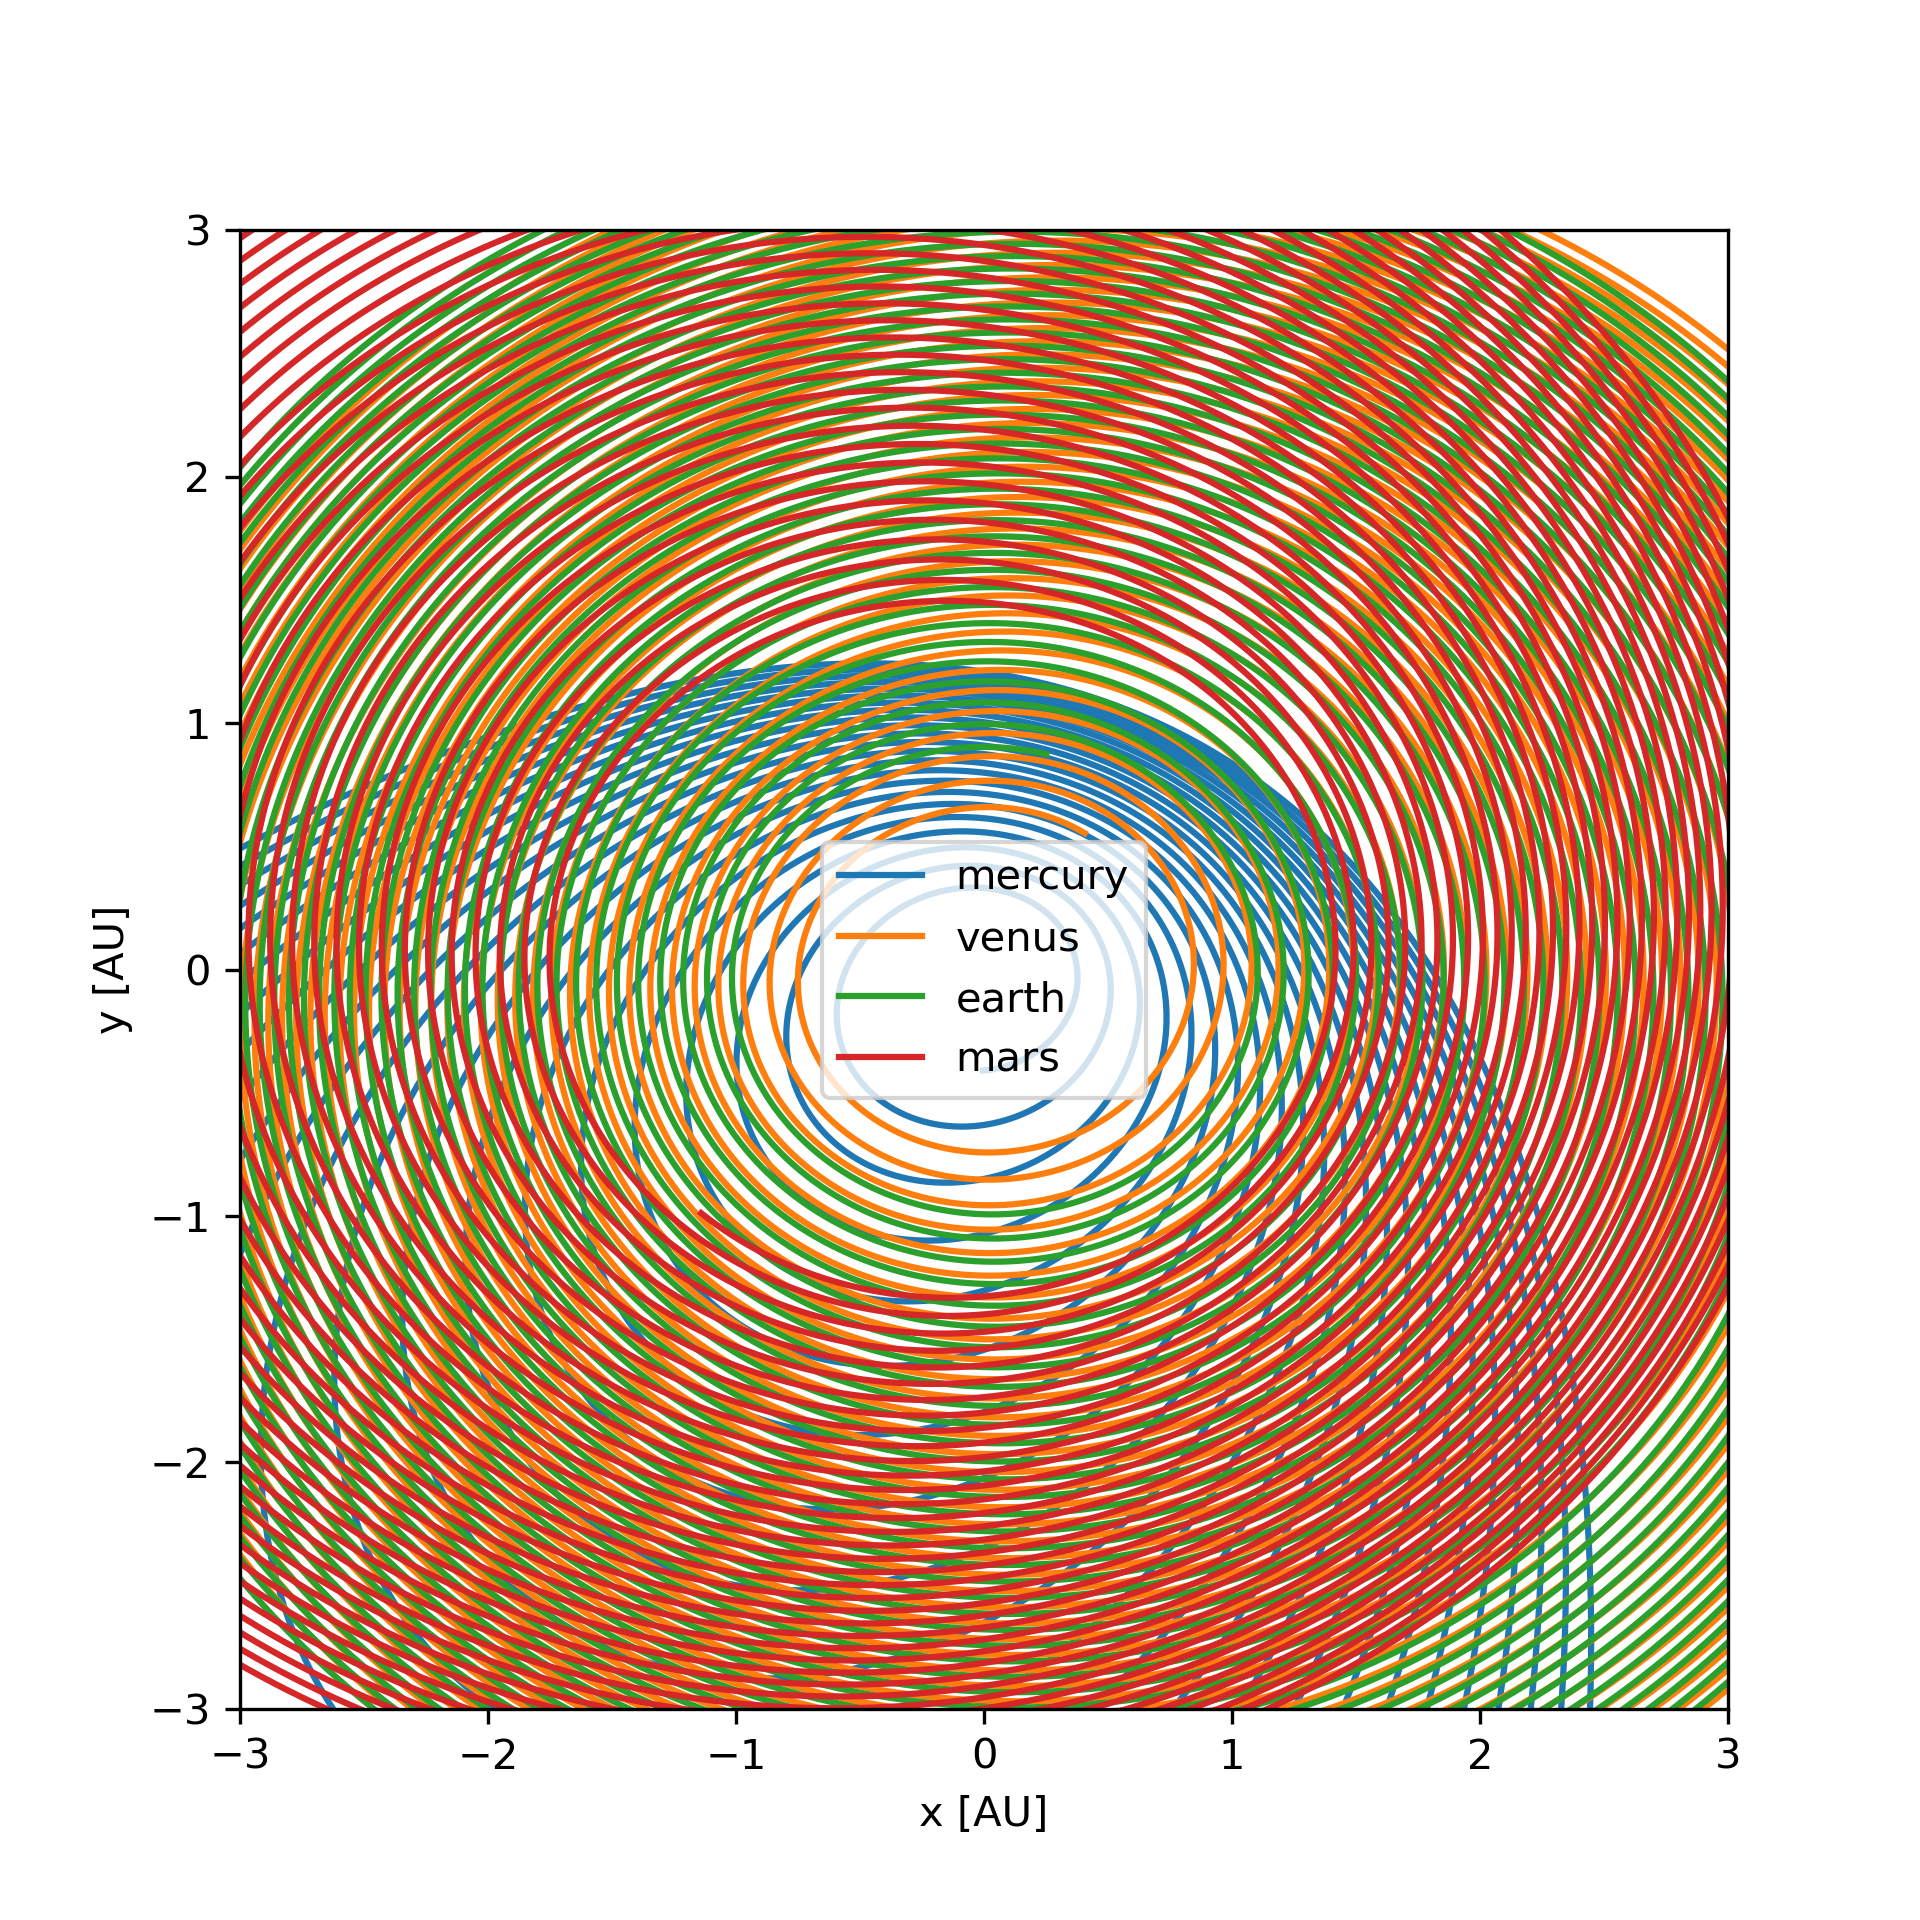
\includegraphics[width=.60\linewidth]{./plots/xy-euler-zoom.png}
  \caption{The evolution of the x and y positions of the 4 inner planets when integrating using Euler's algorithm. We can clearly see the divergence in this plot.}
  \label{fig:xy-eul-zoom}
\end{figure}

\begin{figure}[H]
  \centering
  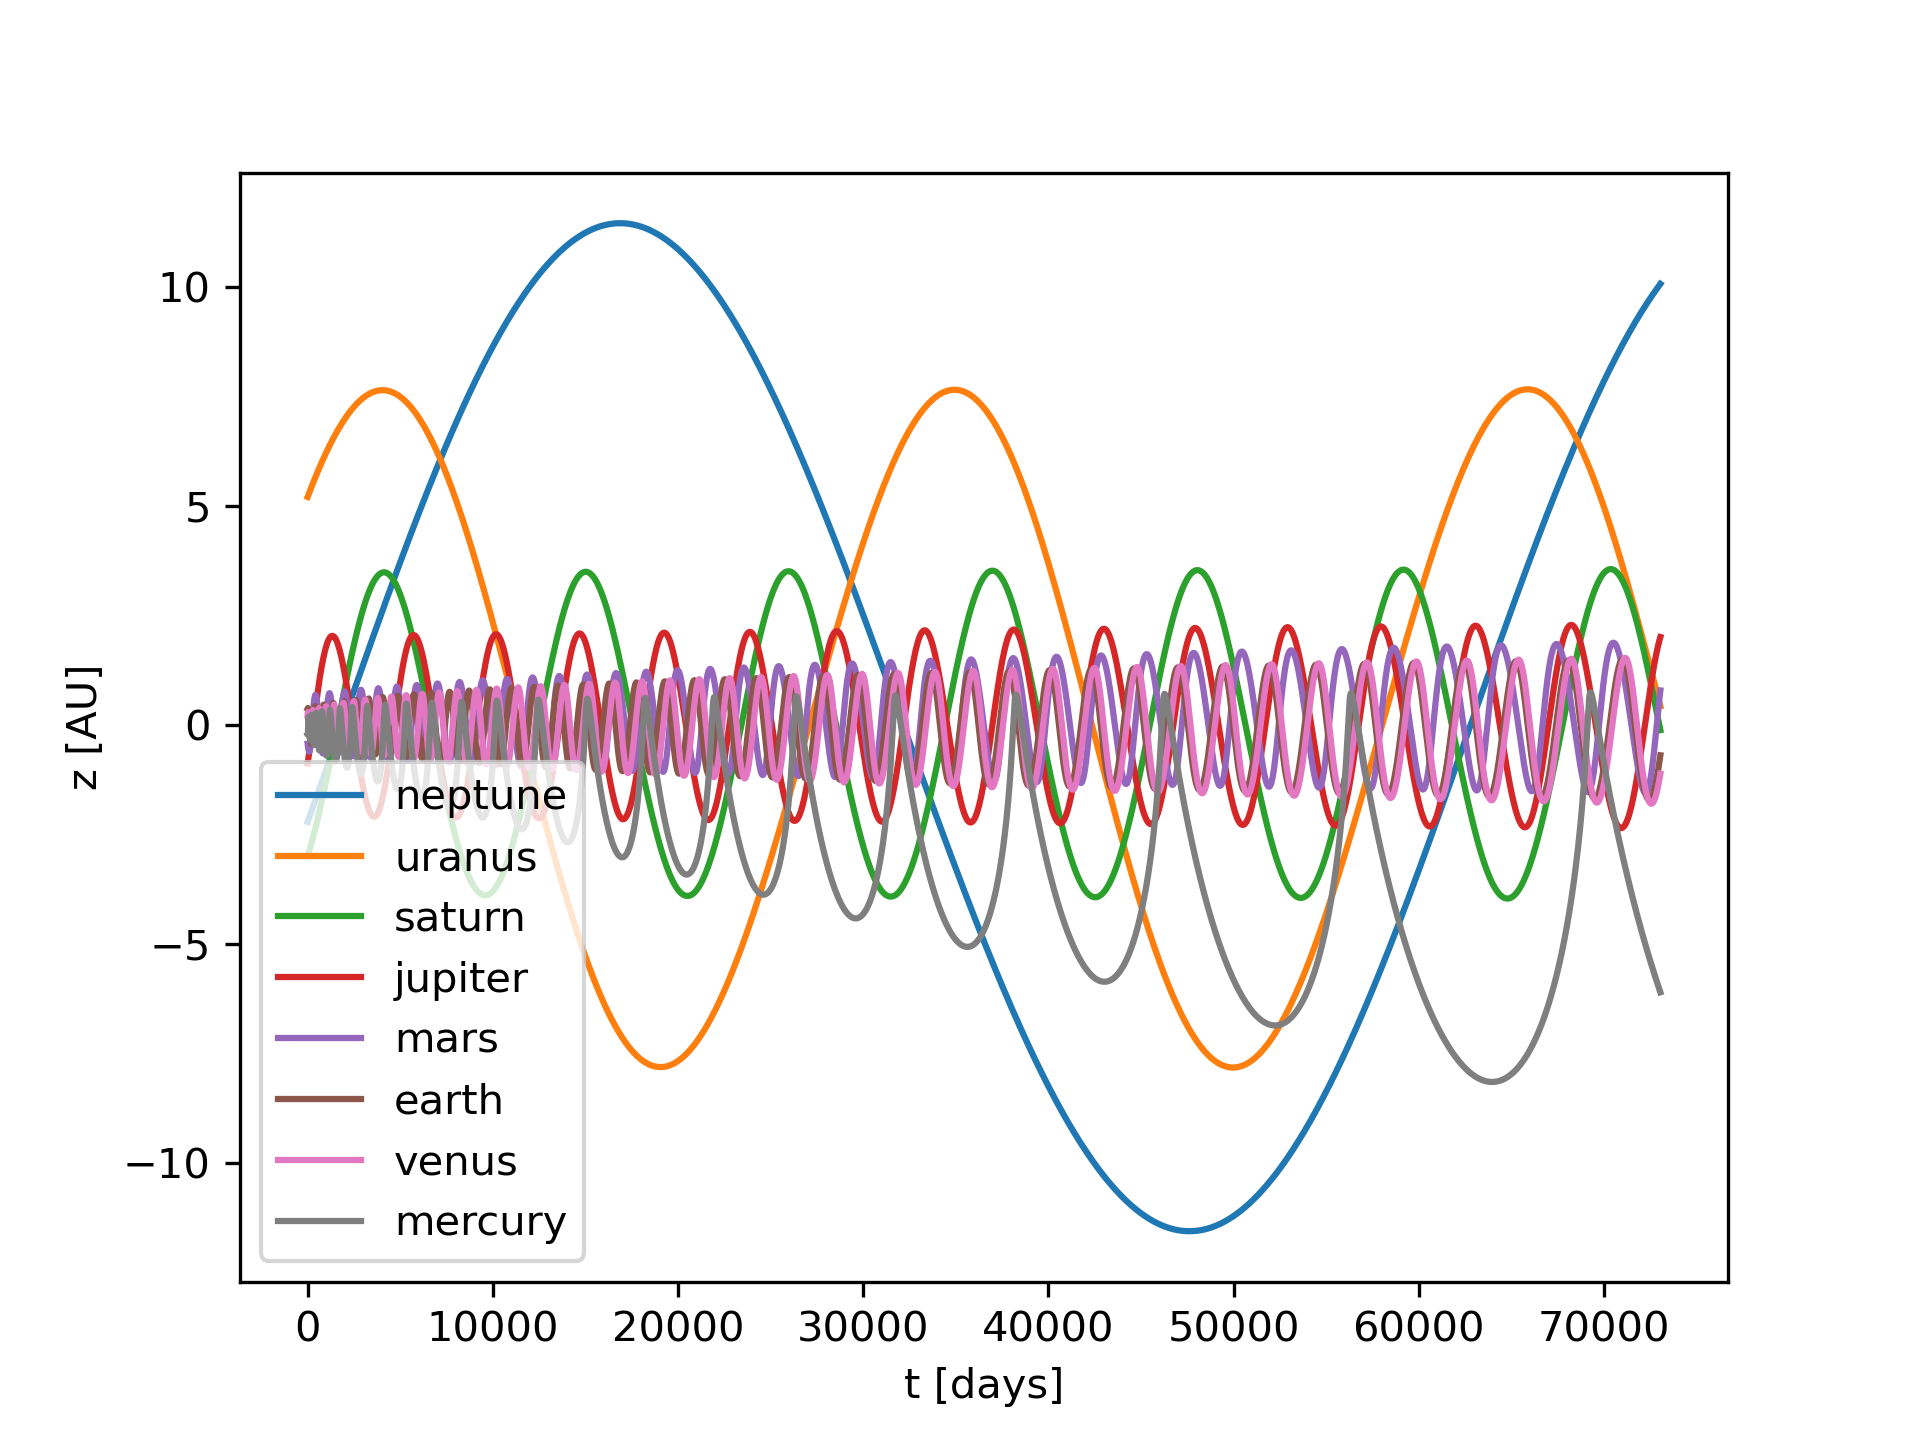
\includegraphics[width=.8\linewidth]{./plots/z-euler.png}
  \caption{The evolution of the z positions of all the 8 planets when integrating using Euler's algorithm. We can see the divergence of the inner planets.}
  \label{fig:z-eul}
\end{figure}

\begin{figure}[H]
  \centering
  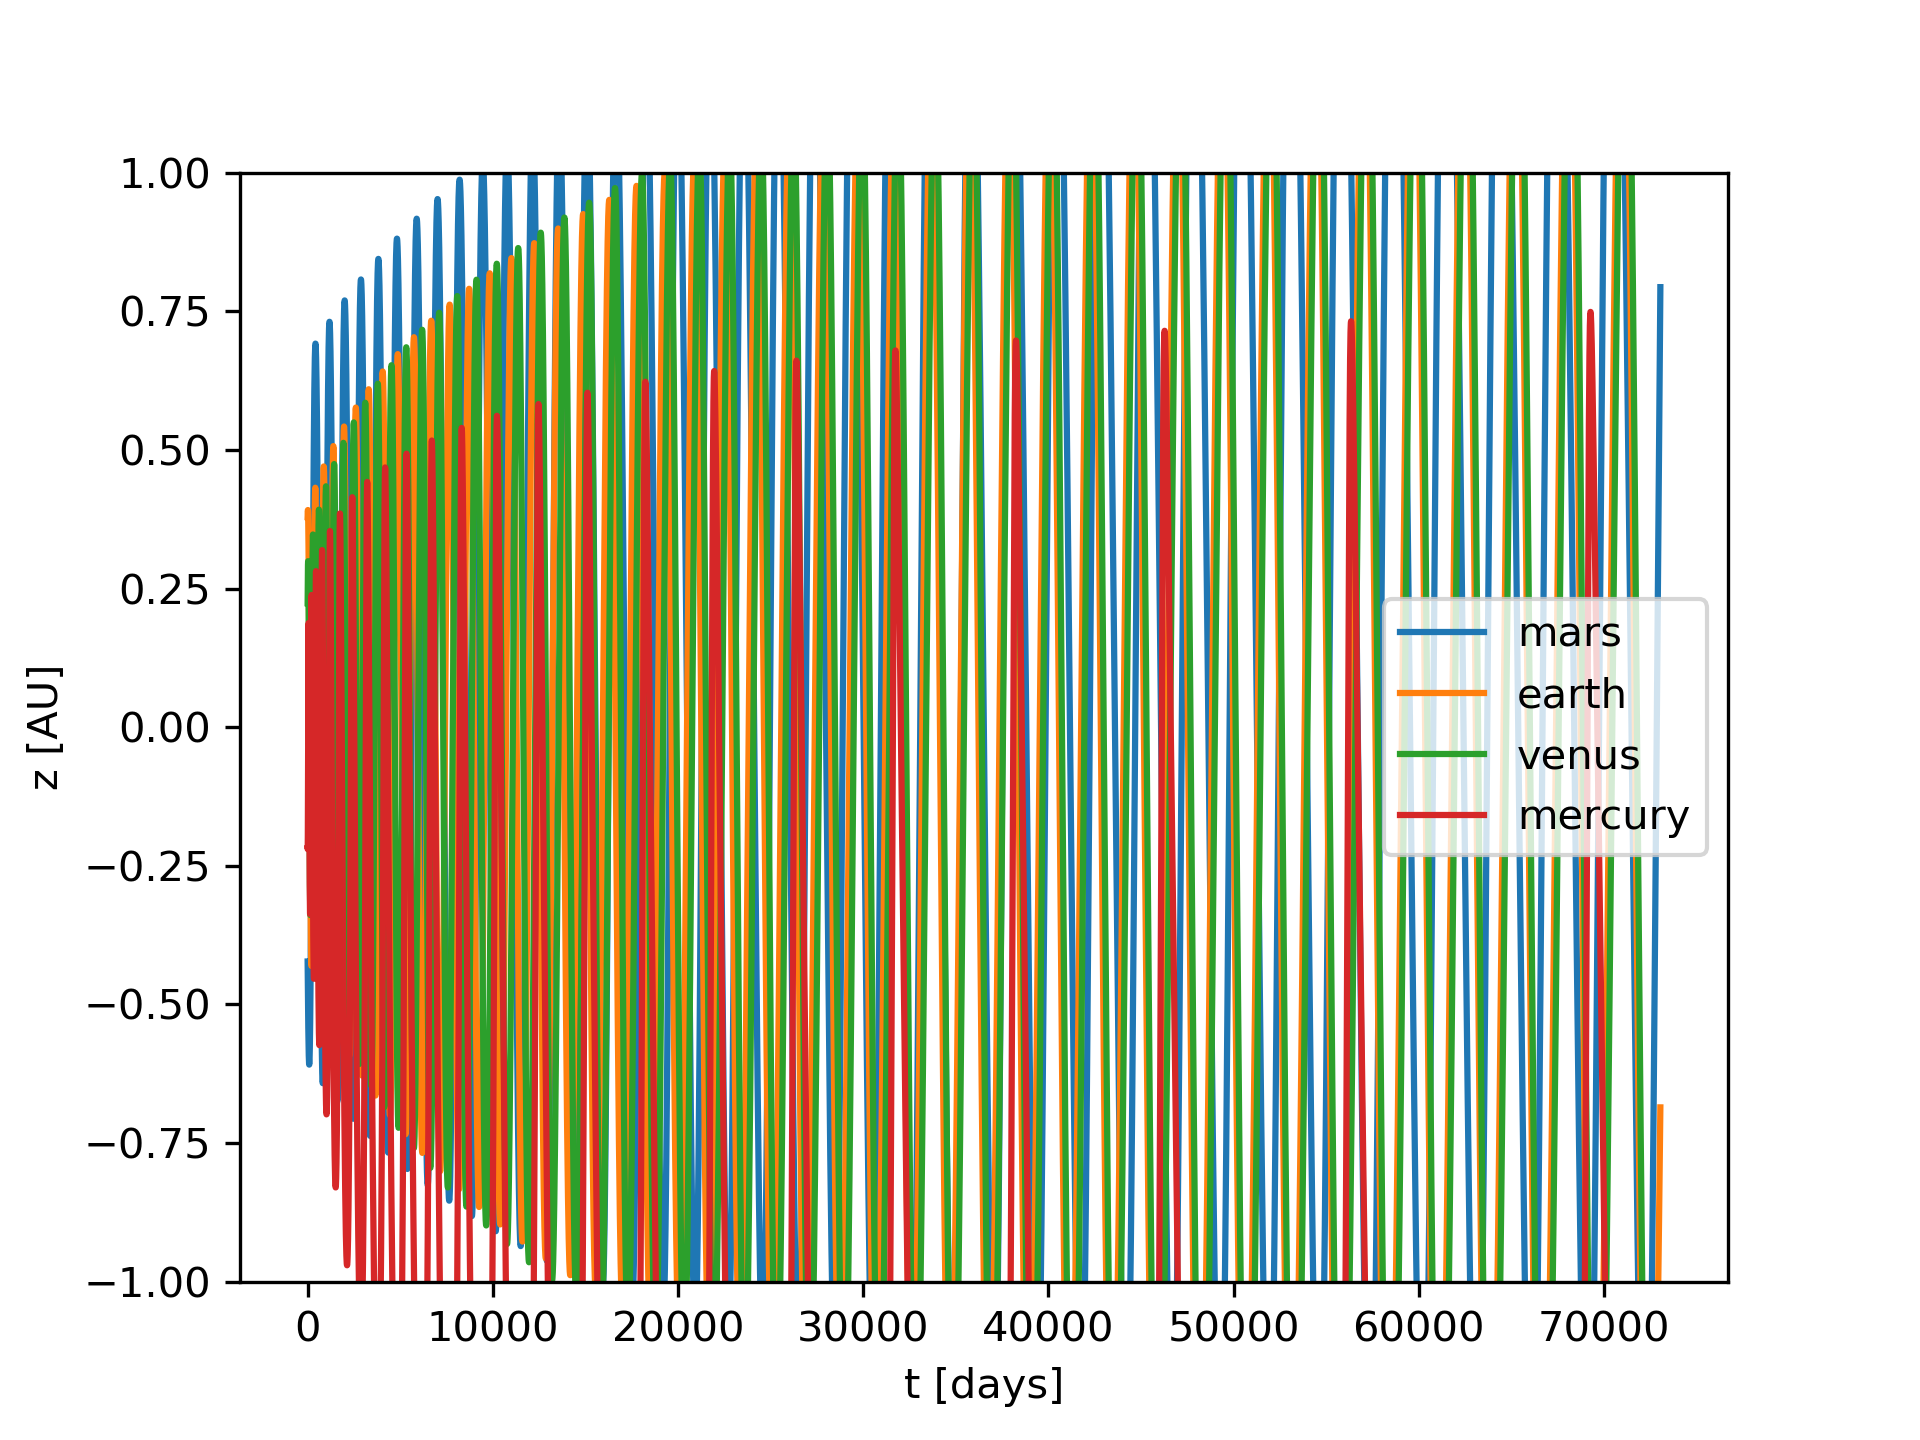
\includegraphics[width=.8\linewidth]{./plots/z-euler-zoom.png}
  \caption{The evolution of the z positions of the 4 inner planets when integrating using Euler's algorithm. We can clearly see the divergence in this plot.}
  \label{fig:z-eul-zoom}
\end{figure}

\begin{figure}[H]
  \centering
  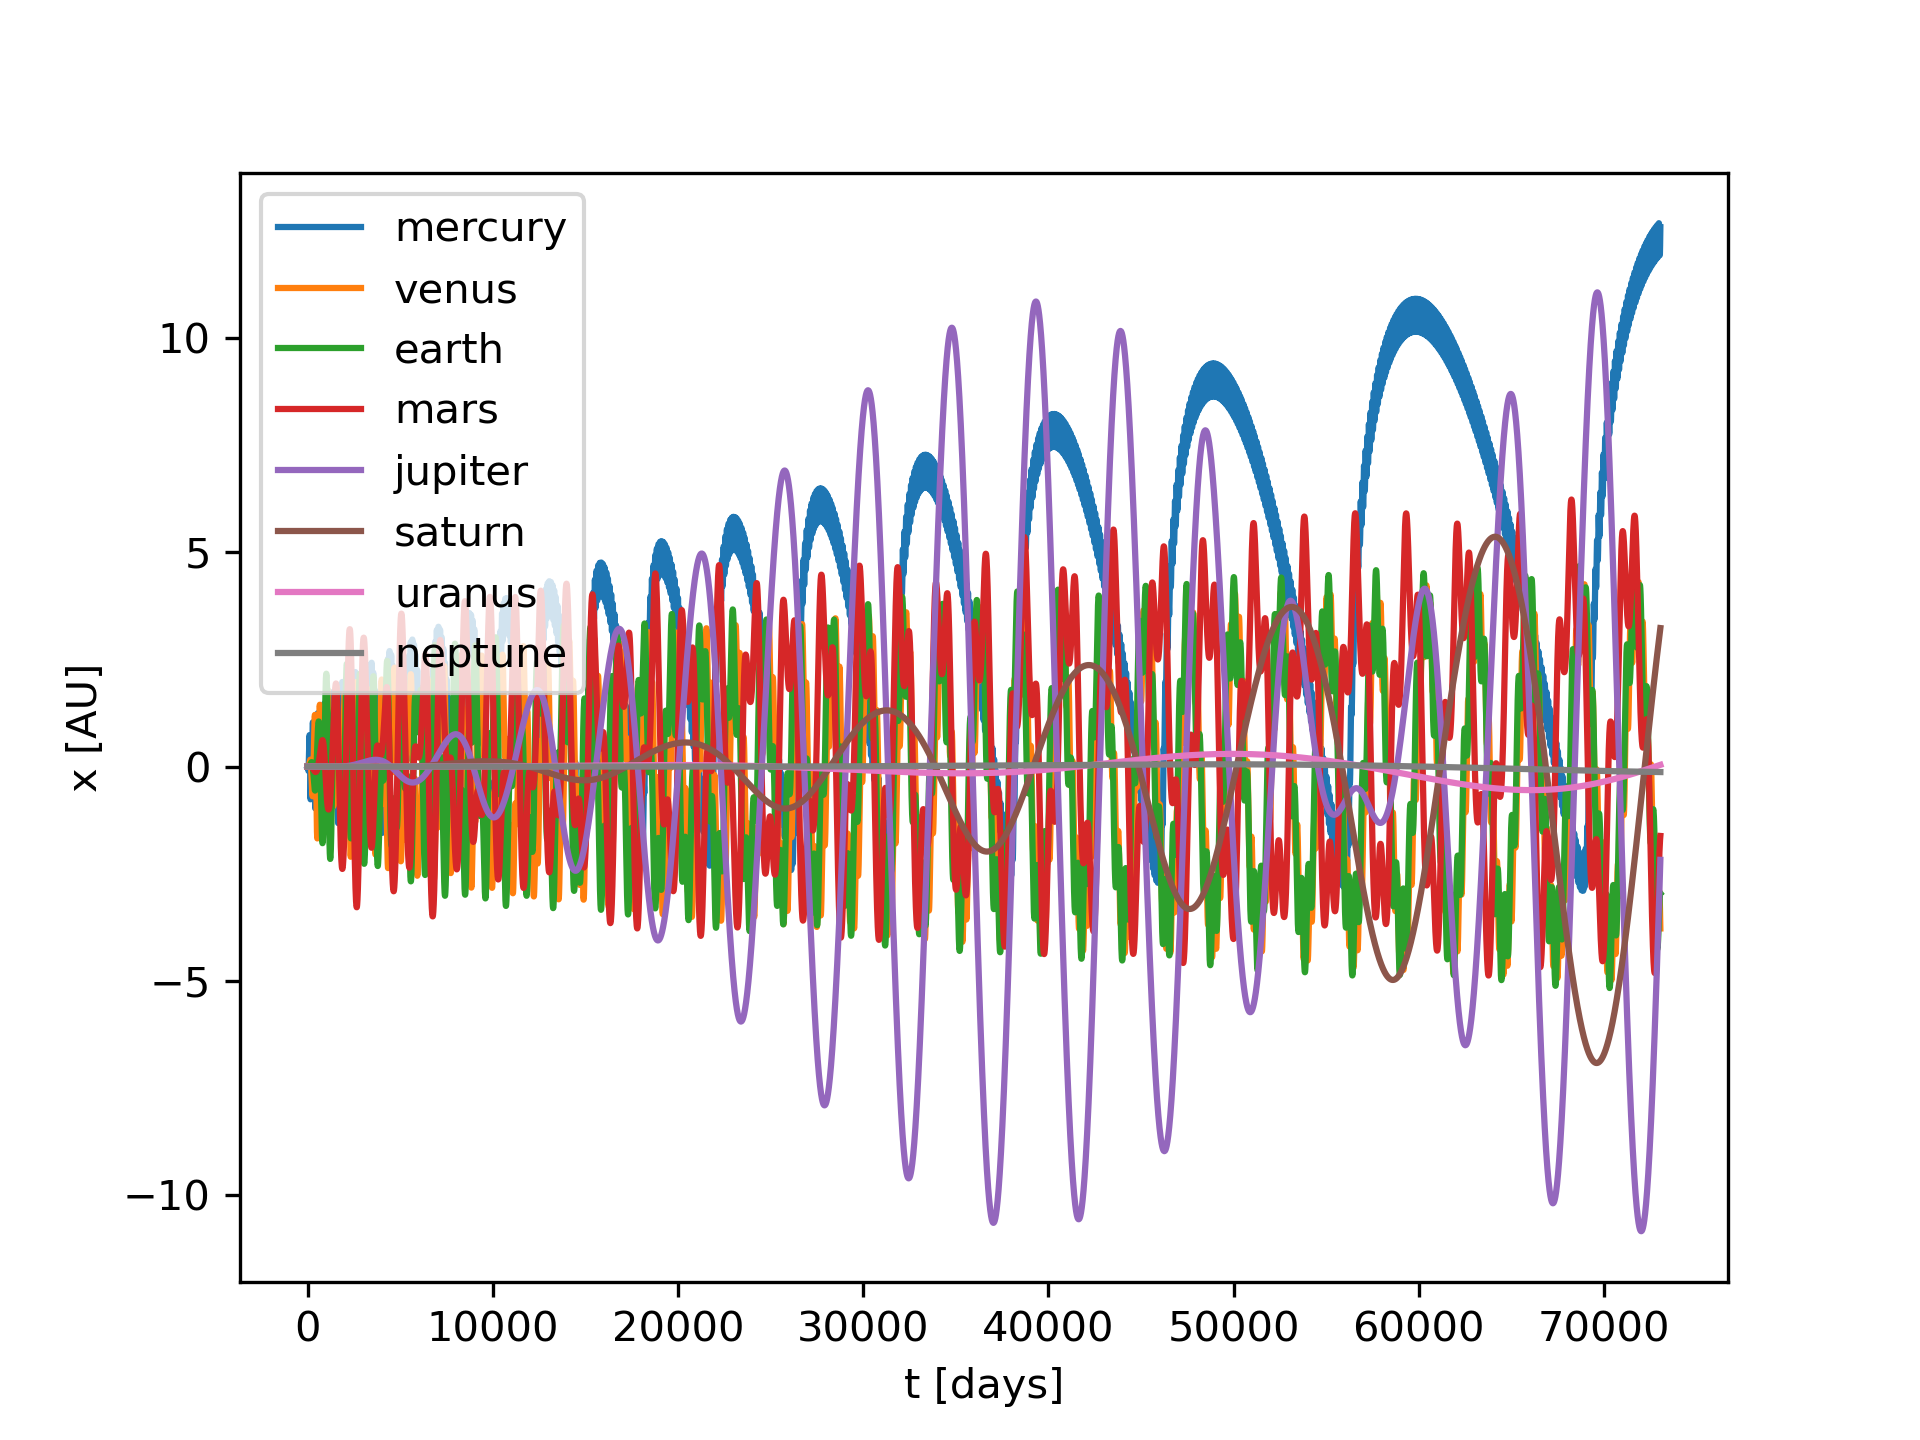
\includegraphics[width=.8\linewidth]{./plots/x-leapfrog-euler.png}
  \caption{The difference in x positions of all the 8 planets when integrating using the Leapfrog minus when integrating with Euler's algorithm. We can also see the divergence of Euler's algorithm at the inner planets in this plot.}
  \label{fig:x-leap-eul}
\end{figure}


\section{Calculating forces with the FFT}

In this section, we will calculate the gravitational forces on a grid of 1024 particles with 1 mass unit each. The volume that we are interested in is periodic, which means that the edges connect. We will perform the calculations in the frequency space and then reconvert it to normal space.

\subsection{Generate and convert}
\label{sec:gen}

We first want to generate the volume with all the densities. We do that with the function ``generate'' which creates a grid $[16 \times 16 \times 16]$ with all the interpolated densities of the particles and also returns the coordinates in a 1D array. 

\lstinputlisting{generate.py}

In the main part of the script we generate the grid and calculate the contrast: $\delta = \frac{\rho-\bar{\rho}}{\bar{\rho}}$. We then create colormap plots for 4 slices which are shown in \Cref{fig:2d_4,fig:2d_9,fig:2d_11,fig:2d_14}


\begin{figure}[H]
  \centering
  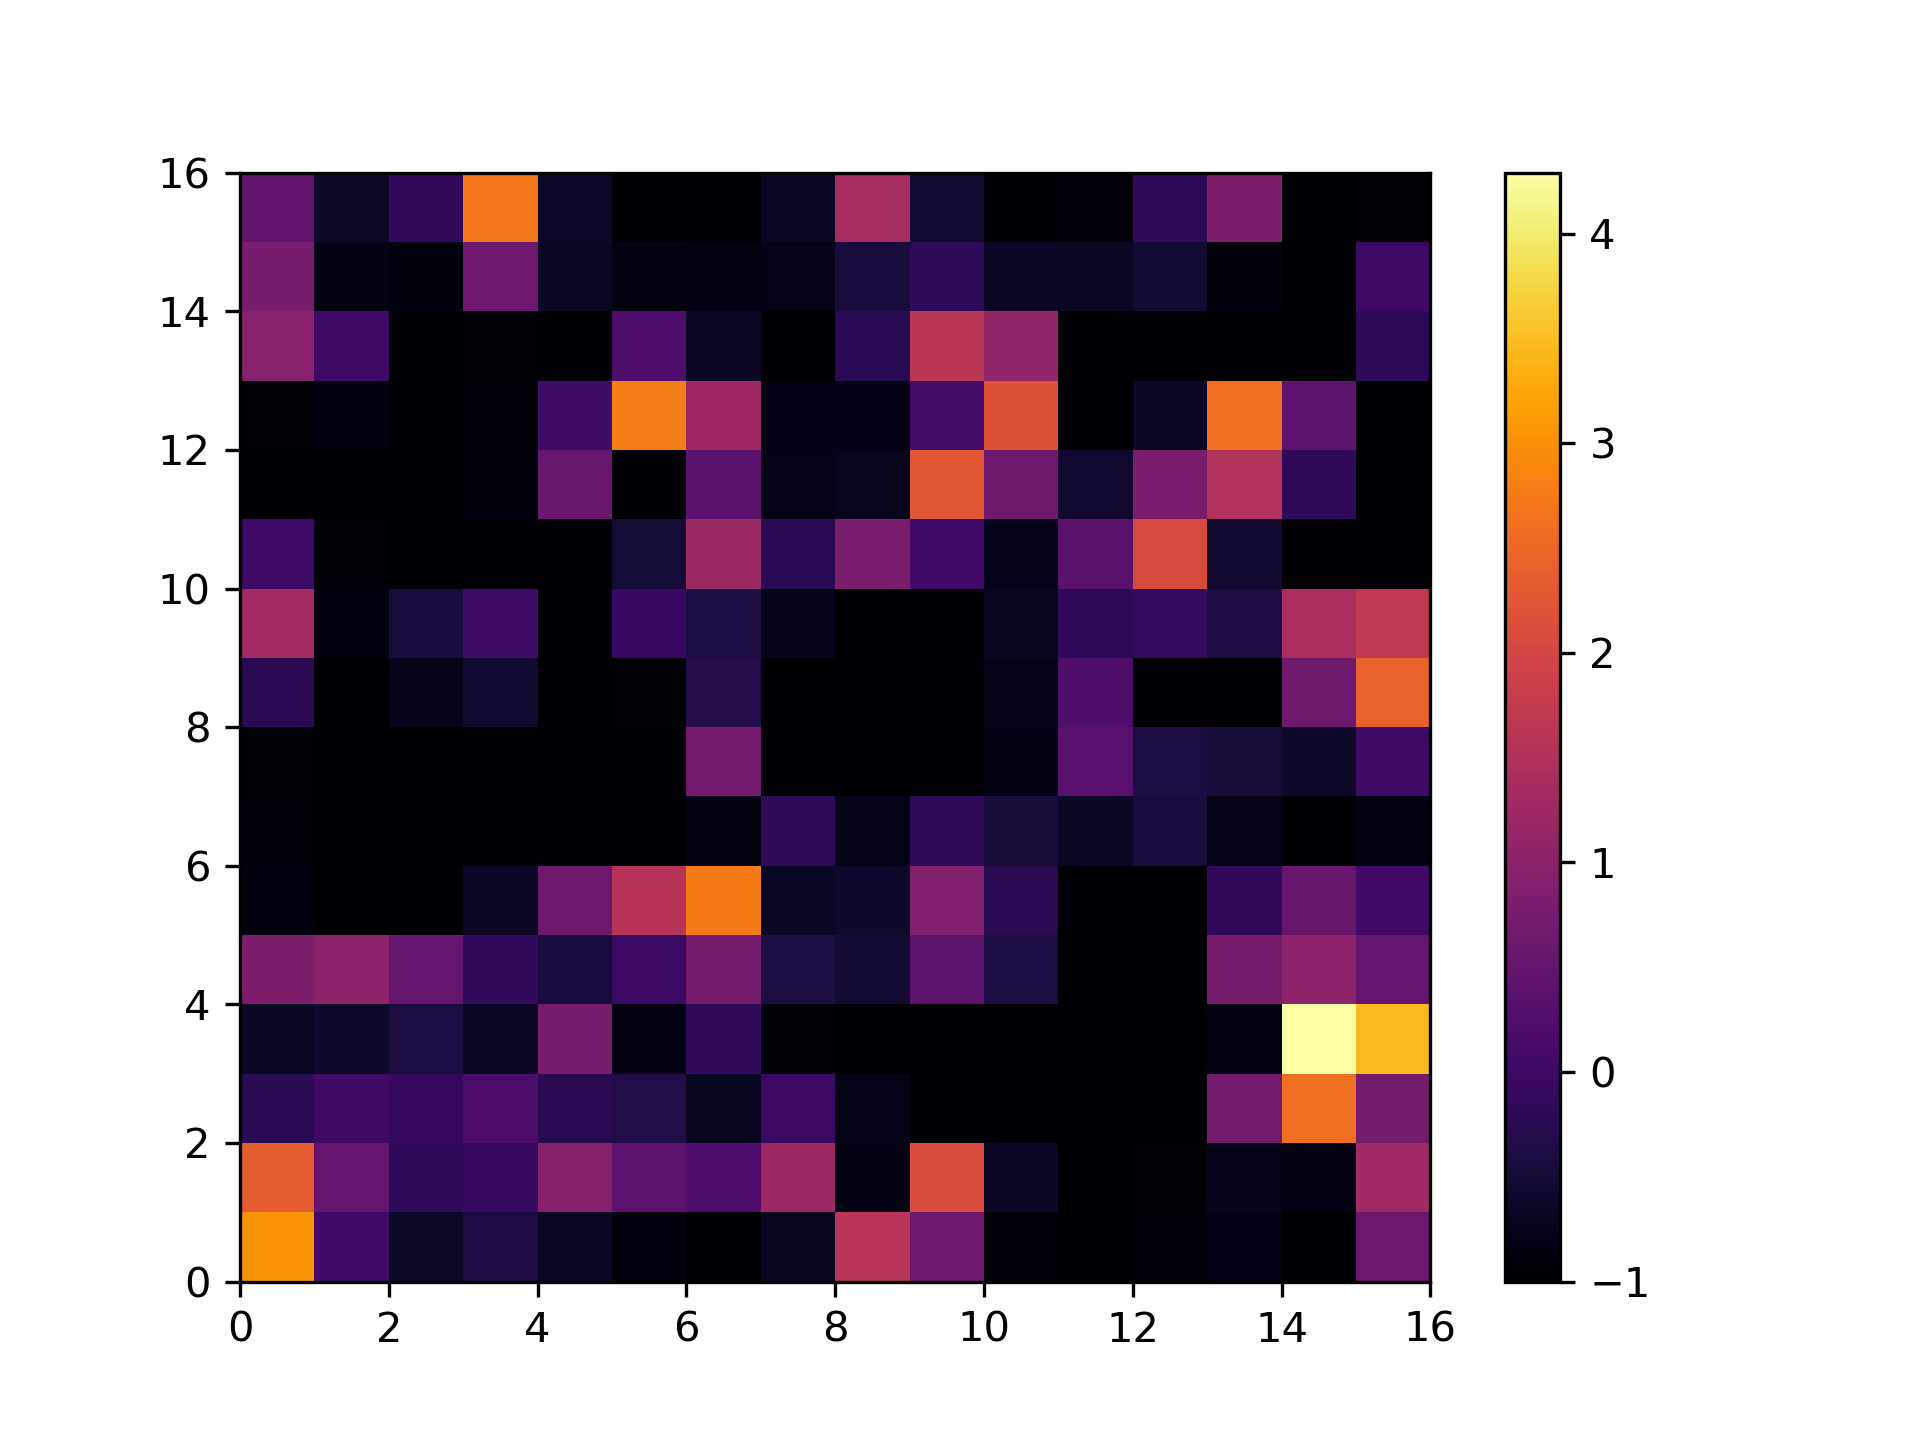
\includegraphics[width=.8\linewidth]{./plots/2d_slice_4.5.png}
  \caption{A 2D slice of the grid at z=4.5}
  \label{fig:2d_4}
\end{figure}

\begin{figure}[H]
  \centering
  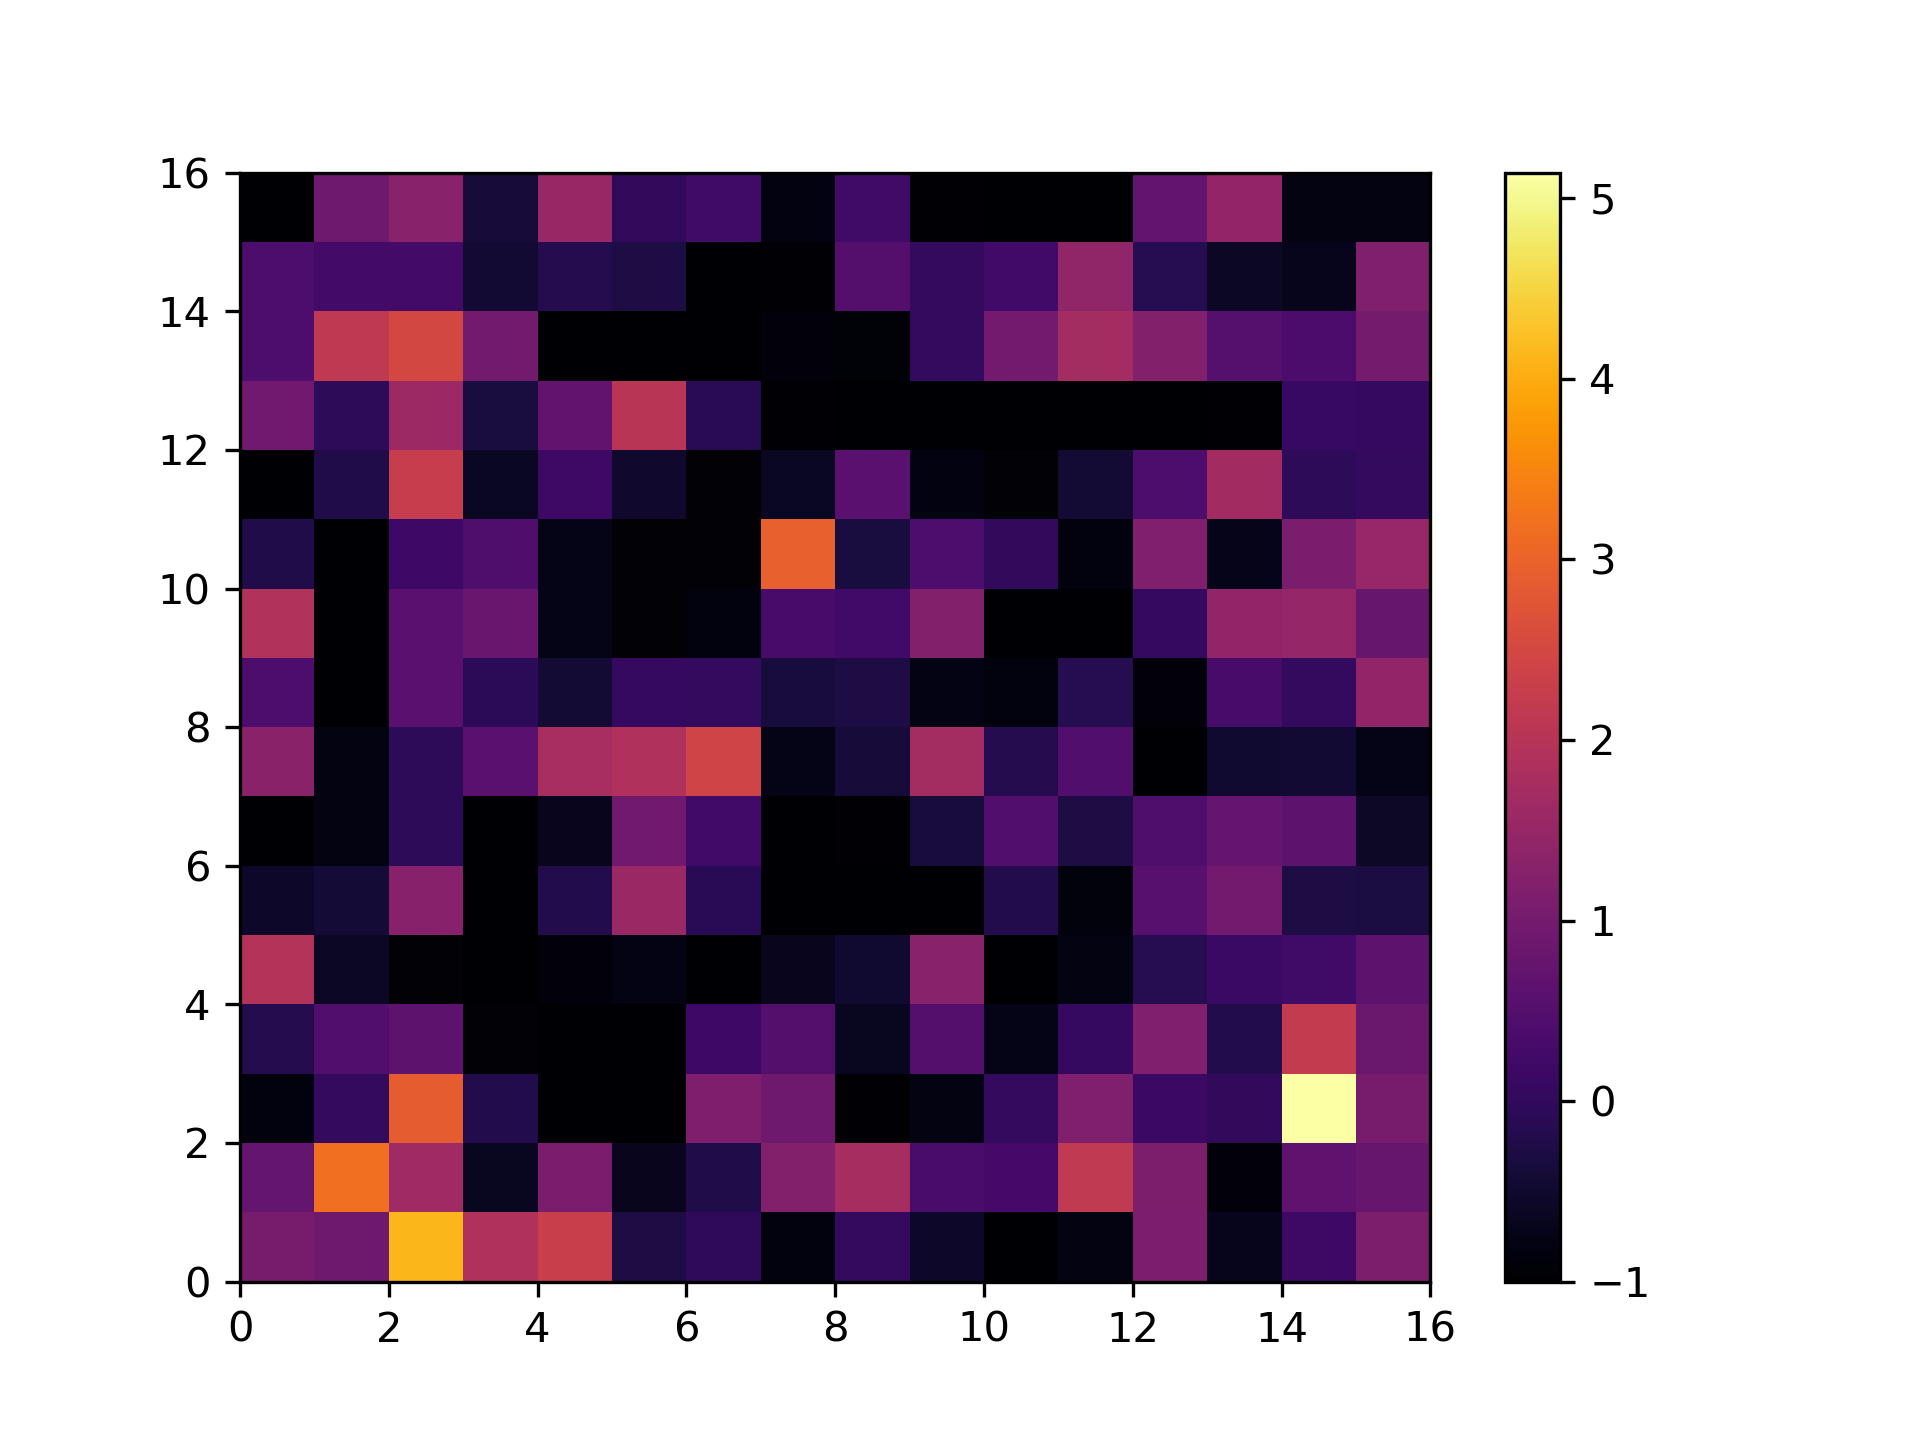
\includegraphics[width=.8\linewidth]{./plots/2d_slice_9.5.png}
  \caption{A 2D slice of the grid at z=9.5}
  \label{fig:2d_9}
\end{figure}

\begin{figure}[H]
  \centering
  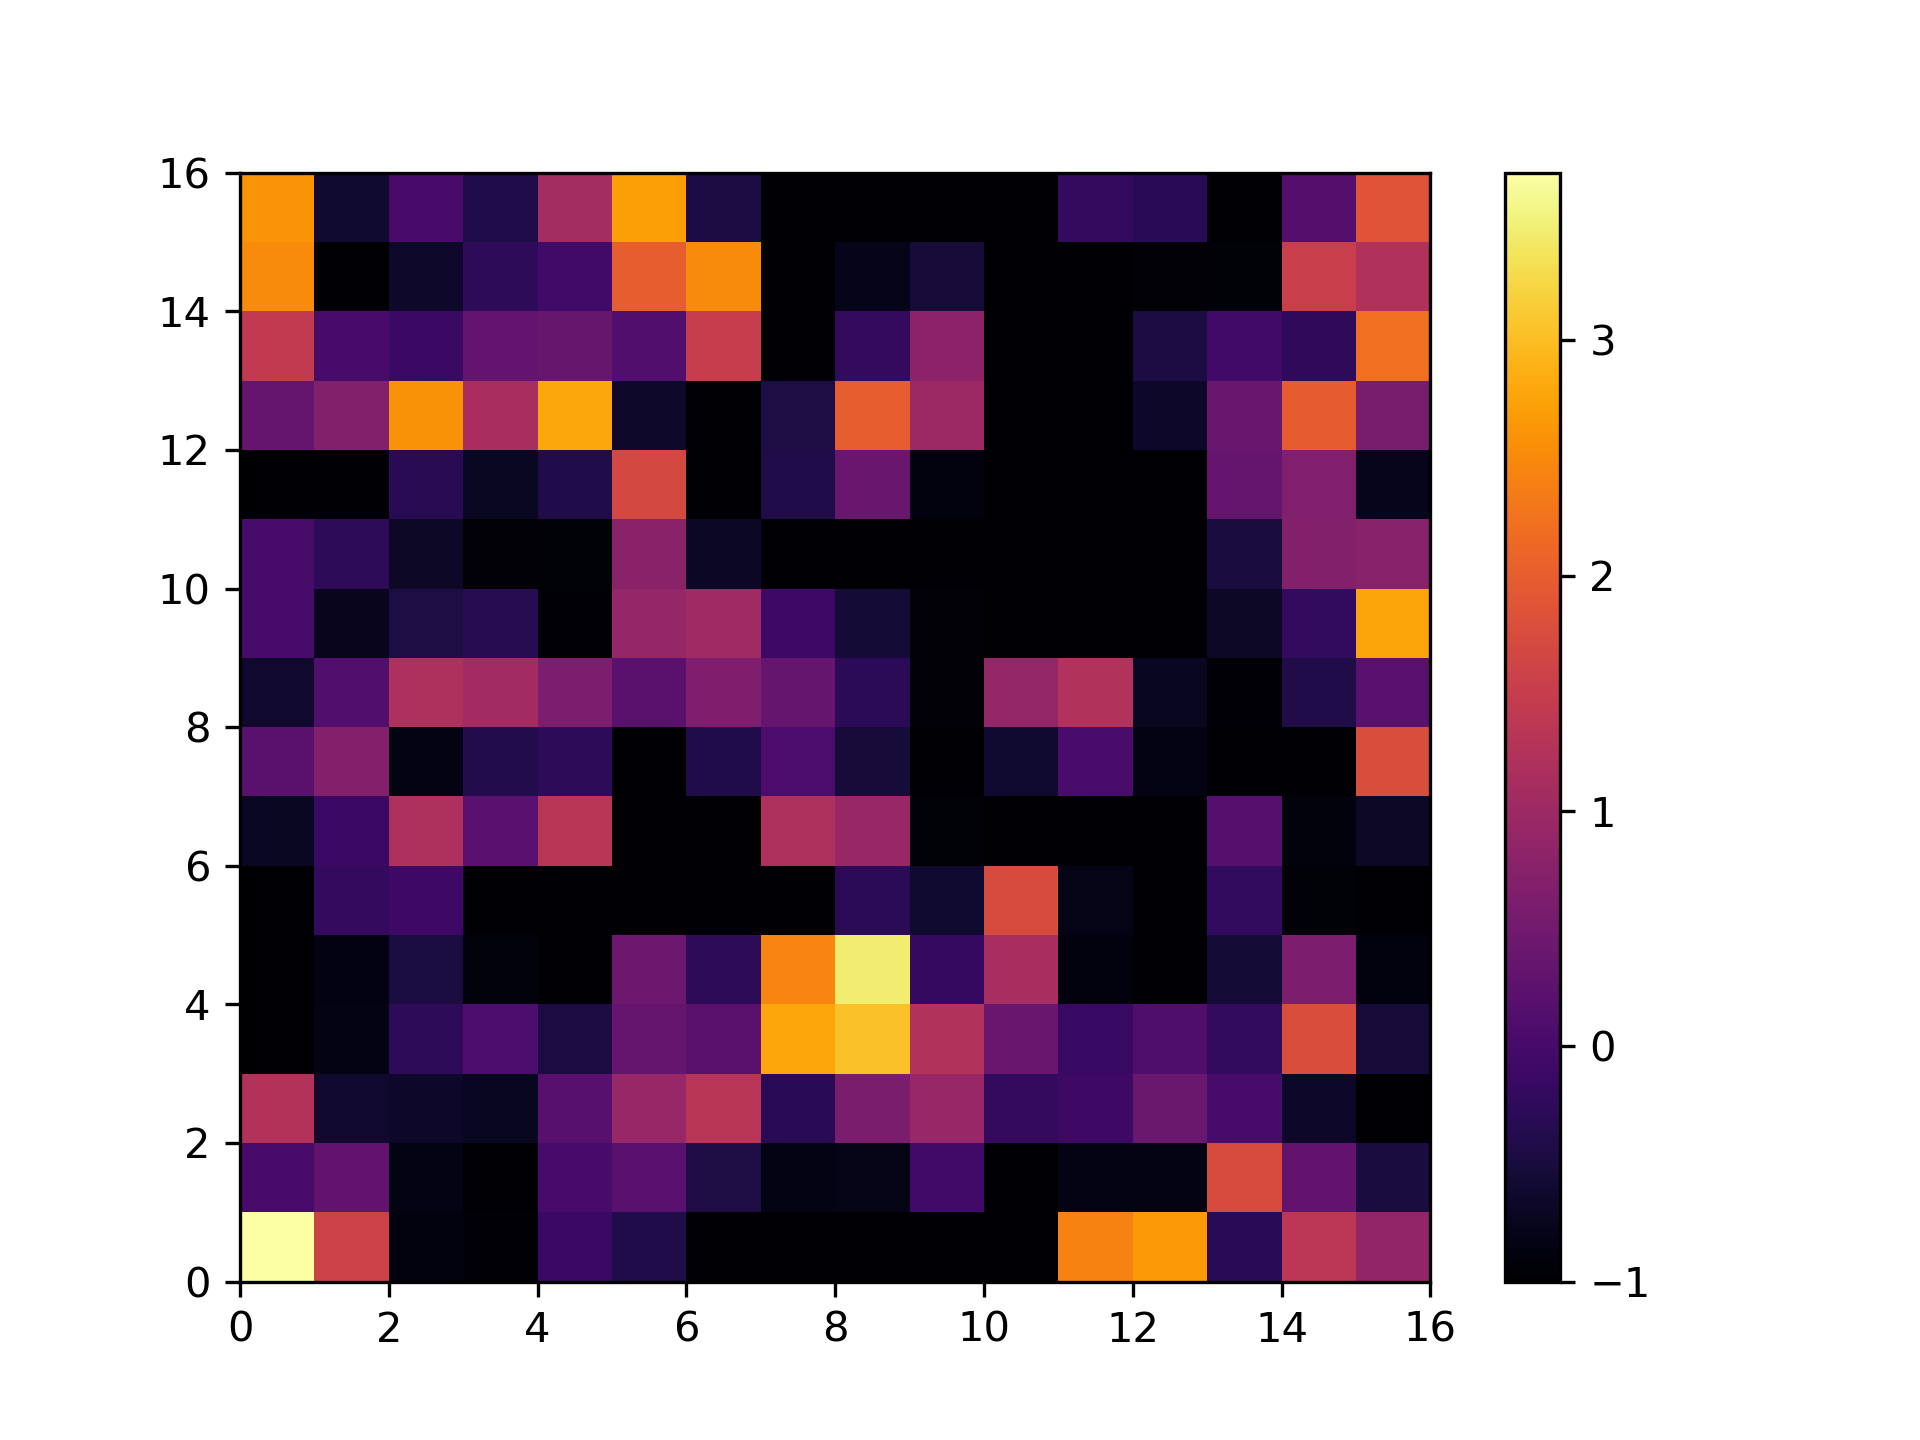
\includegraphics[width=.8\linewidth]{./plots/2d_slice_11.5.png}
  \caption{A 2D slice of the grid at z=11.5}
  \label{fig:2d_11}
\end{figure}

\begin{figure}[H]
  \centering
  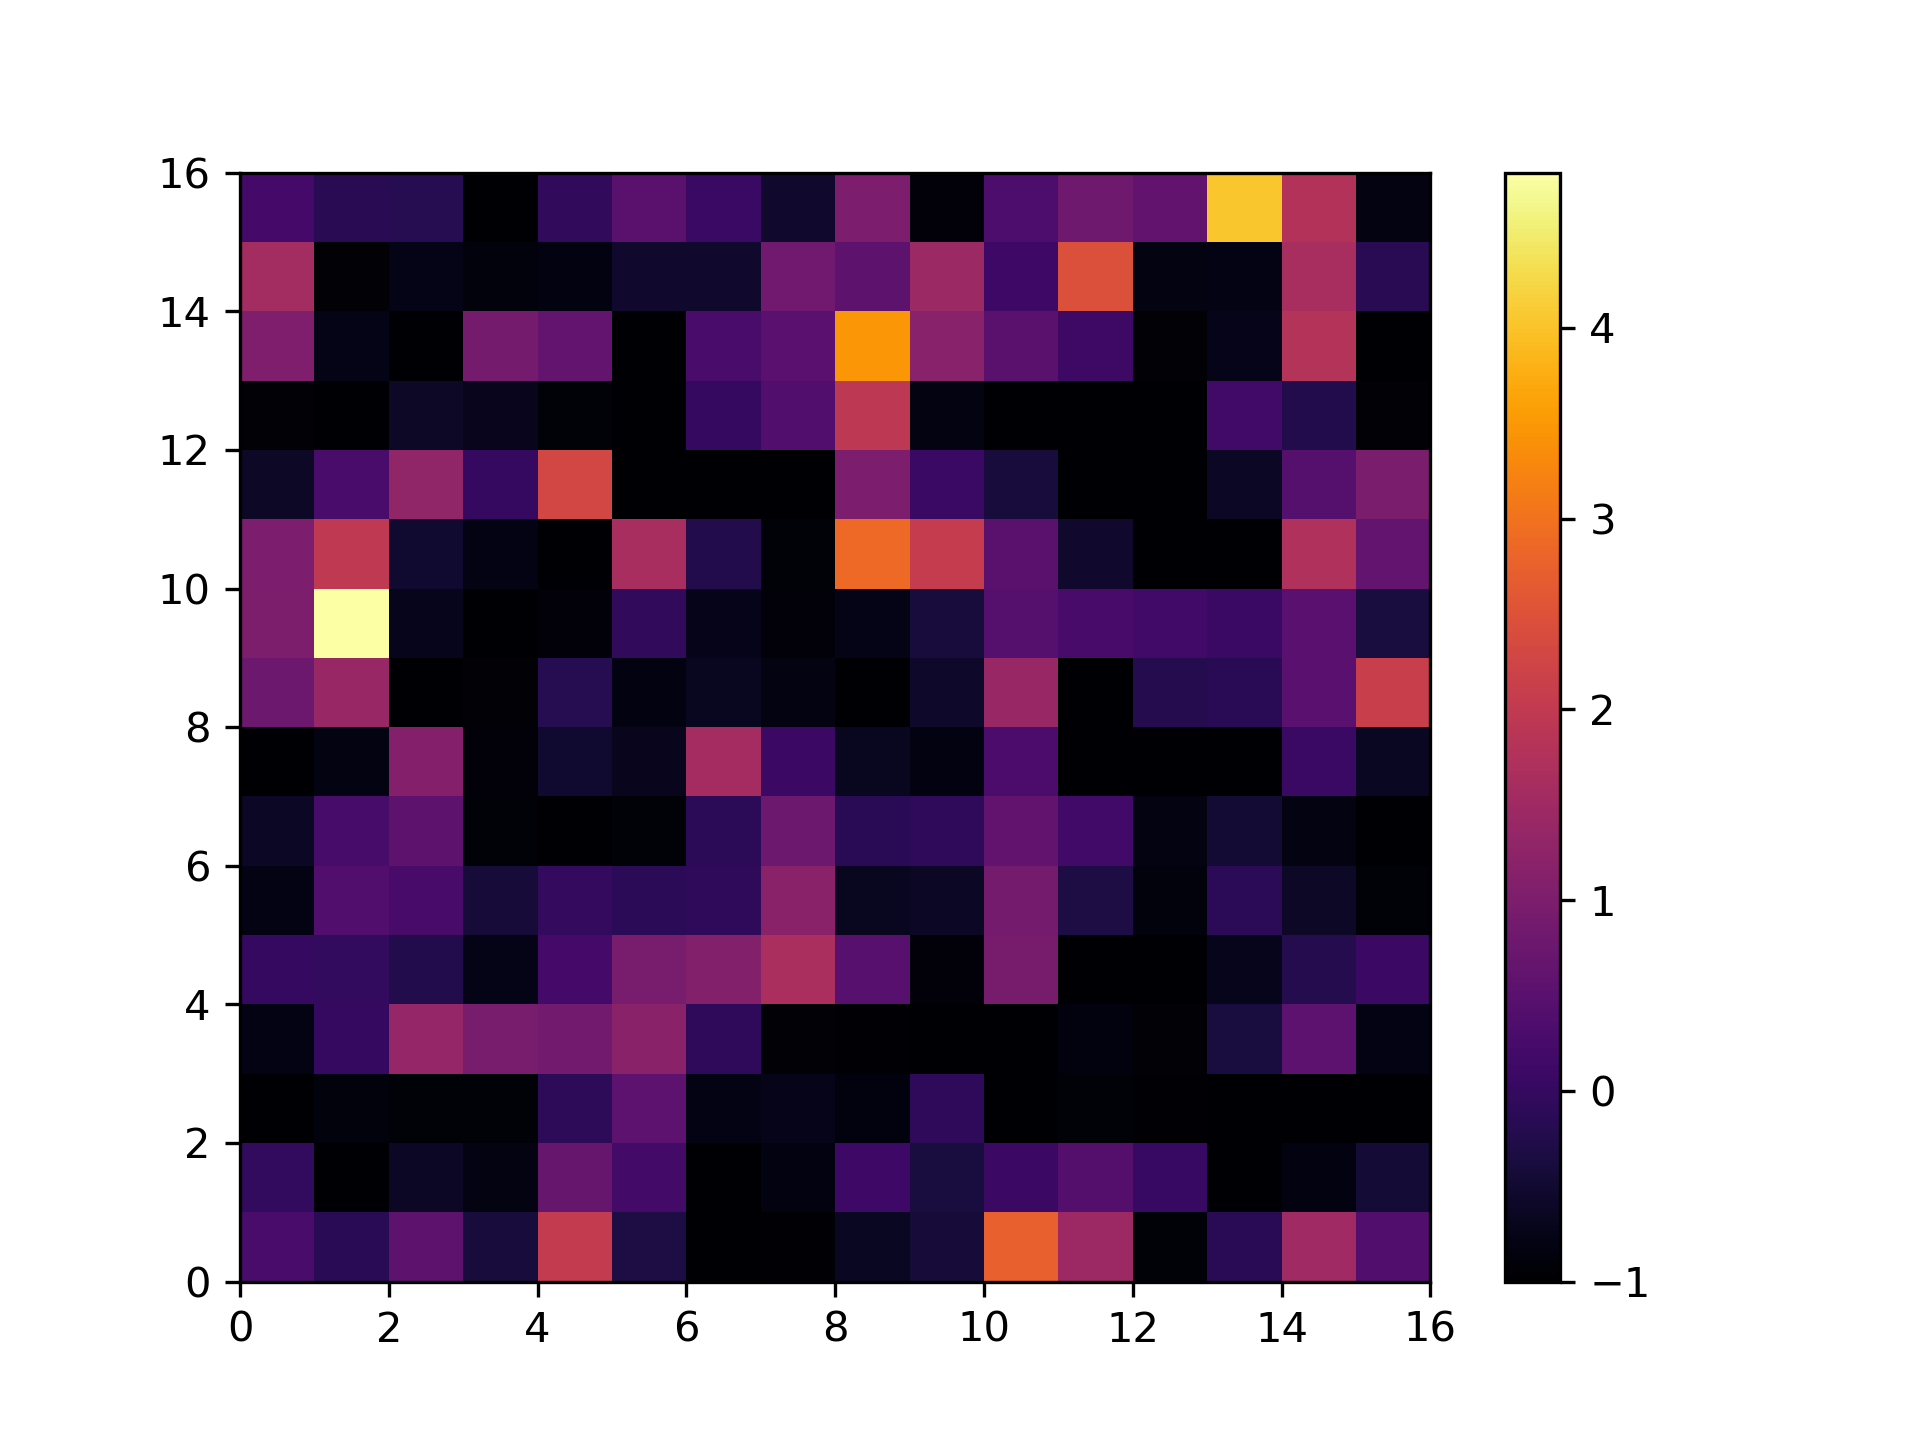
\includegraphics[width=.8\linewidth]{./plots/2d_slice_14.5.png}
  \caption{A 2D slice of the grid at z=14.5}
  \label{fig:2d_14}
\end{figure}

\subsection{Calculate gravitational forces}

We now want to calculate the gravitational potential at each grid point. The Poisson equation is:
\begin{equation}
  \nabla^2 \Phi = 4 \pi G \bar{\rho}(1+\delta) \propto \delta
\end{equation}
We can calculate the potential in Fourier space 
\begin{equation}
  \label{eq:four_pot}
  -k^2 \tilde{\Phi} \propto \tilde{\delta}
\end{equation}
The negative sign ensures that high-mass regions will have a smaller potential as is the convention for all gravitational potentials. By doing this we can find the Fourier-transformed potential ($\tilde{\Phi}$) and then with the inverse Fourier-transformation find the real potential ($\Phi$).

To perform the calculations we create an FFT routine using the Cooley-Tukey algorithm. Our function ``cooley\_tukey\_fft'' calls itself recursively on a slice of the input array with all the even elements and another recursive call on all odd elements. When the recursive calls terminate we loop over k to calculate the Fourier transformation. From all the different definitions for the Fourier, we use
\begin{equation}
  \tilde{x}[k] = \sum_{n=0}^{N-1} x[n] e^{-i 2 \pi k \frac{n}{N}}
\end{equation}
where we use a summation because we have a discrete Fourier transformation.

We then create ``cooley\_tukey\_ifft'' in a similar way to perform the inverse FFT calculations. The difference here is the sign at the calculations of the exponential. We also have to normalize the results, by dividing by 2. The reason for that is that the FFT operation gives a symmetrical result for positive and negative frequencies, which makes our inverse FFT have double the original amplitude if we don't normalize it.

The grid we want to use FFT on is in 3 dimensions. Our functions only operate in one dimension so we create 2 similar functions ``fft\_3d'' and ``ifft\_3d'' that utilize the previous functions to perform a 3D Fourier and inverse Fourier transformation. The way they operate is that they slice the 3D grid into multiple 2D slices, and they perform a 2D Fourier transformation. The 2D Fourier transformation is simple as we can just take the FFT of all the rows followed by the FFT of all the columns. After having the FFT of all the slices we can take the 1D FFT of all the columns in the 3rd dimension. The final result is the 3D FFT of the whole grid. 

\lstinputlisting{fft.py}

In the main part of the script, we calculate the contrast in the same way we did at \Cref{sec:gen}. We then take the 3D FFT of that result. We now want to calculate the Fourier-transformed potential ($\tilde{\Phi}$) using \Cref{eq:four_pot}. For that, we need to calculate the wavenumber $k$ for each position in the Fourier-transformed density grid. Because of symmetries in our FFT routine, the results are returned with first the term for k=0 followed by all the positive terms of k. At $\tilde{x}[n/2]$ we have our greatest positive frequency term and then we begin with the negative ones starting from the smallest value. We create 3 arrays for all the 3 dimensions of our grid using this definition and then create a grid for each of the individual components (KX, KY, KZ). Because we have to divide our Fourier transformed densities with the square of the norm of the wavenumber vector we will come across some 0 terms. To avoid any errors we add a sufficiently small value. 

We then take the inverse FFT of the Fourier-transformed potential and take the real part. The new grid array now contains the full potential of the original grid. We create plots for the same 2D slices we used in \Cref{sec:gen} for the potential (\Cref{fig:for_4,fig:for_9,fig:for_11,fig:for_14}) and for the logarithm of the absolute value of the Fourier-transformed potential (\Cref{fig:four_4,fig:four_9,fig:four_11,fig:four_14}). 

\begin{figure}[H]
  \centering
  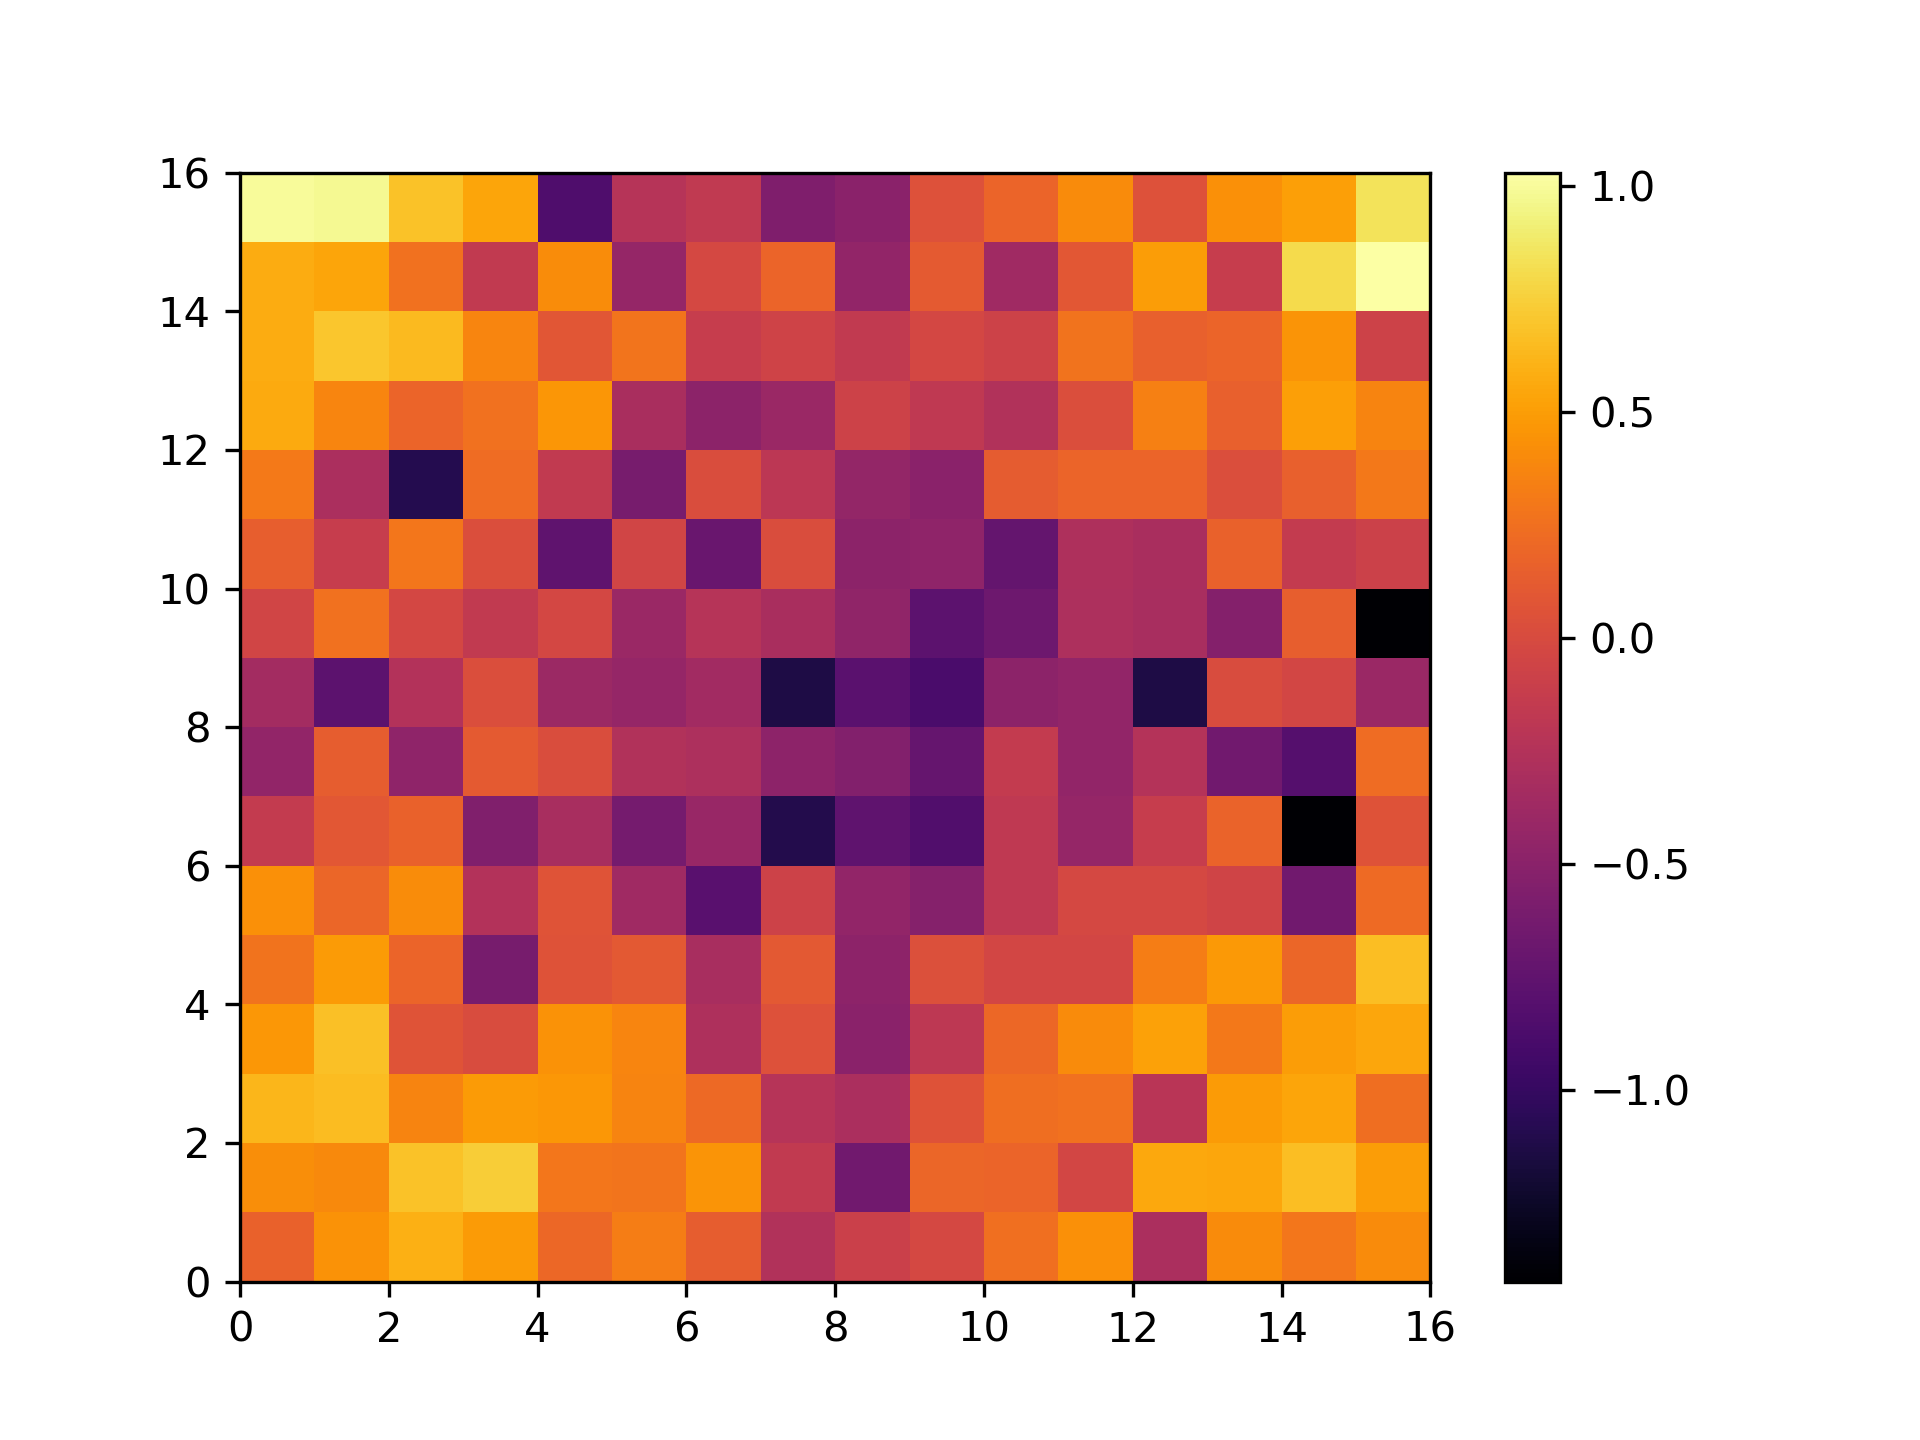
\includegraphics[width=.8\linewidth]{./plots/fourier_4.5.png}
  \caption{A 2D slice of the logarithm of the absolute value of the Fourier-transformed potential at z=4.5}
  \label{fig:four_4}
\end{figure}

\begin{figure}[H]
  \centering
  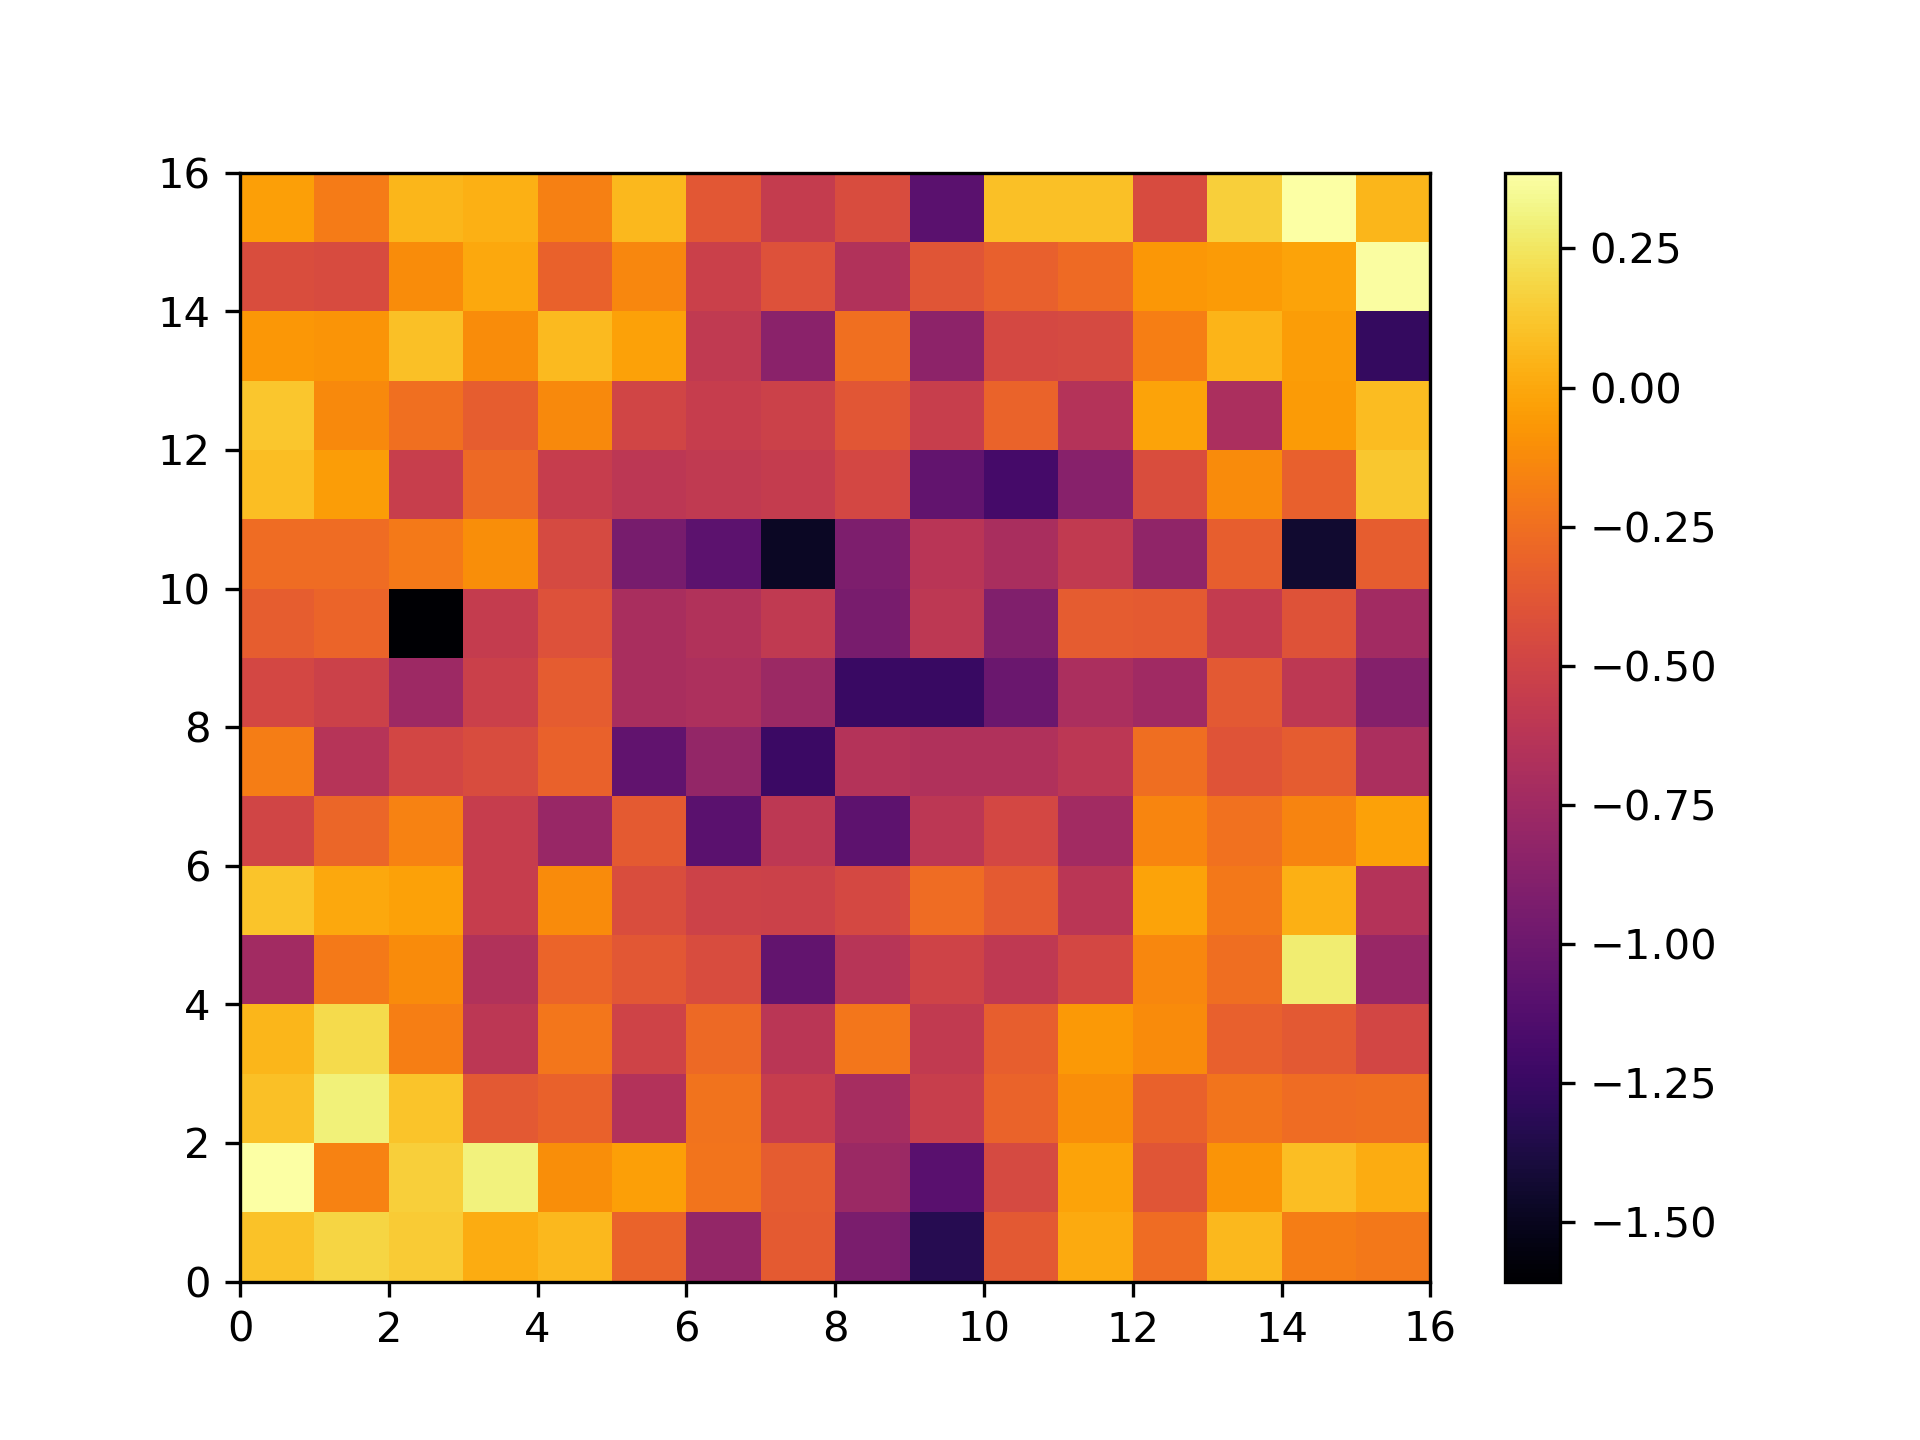
\includegraphics[width=.8\linewidth]{./plots/fourier_9.5.png}
  \caption{A 2D slice of the logarithm of the absolute value of the Fourier-transformed potential at z=9.5}
  \label{fig:four_9}
\end{figure}

\begin{figure}[H]
  \centering
  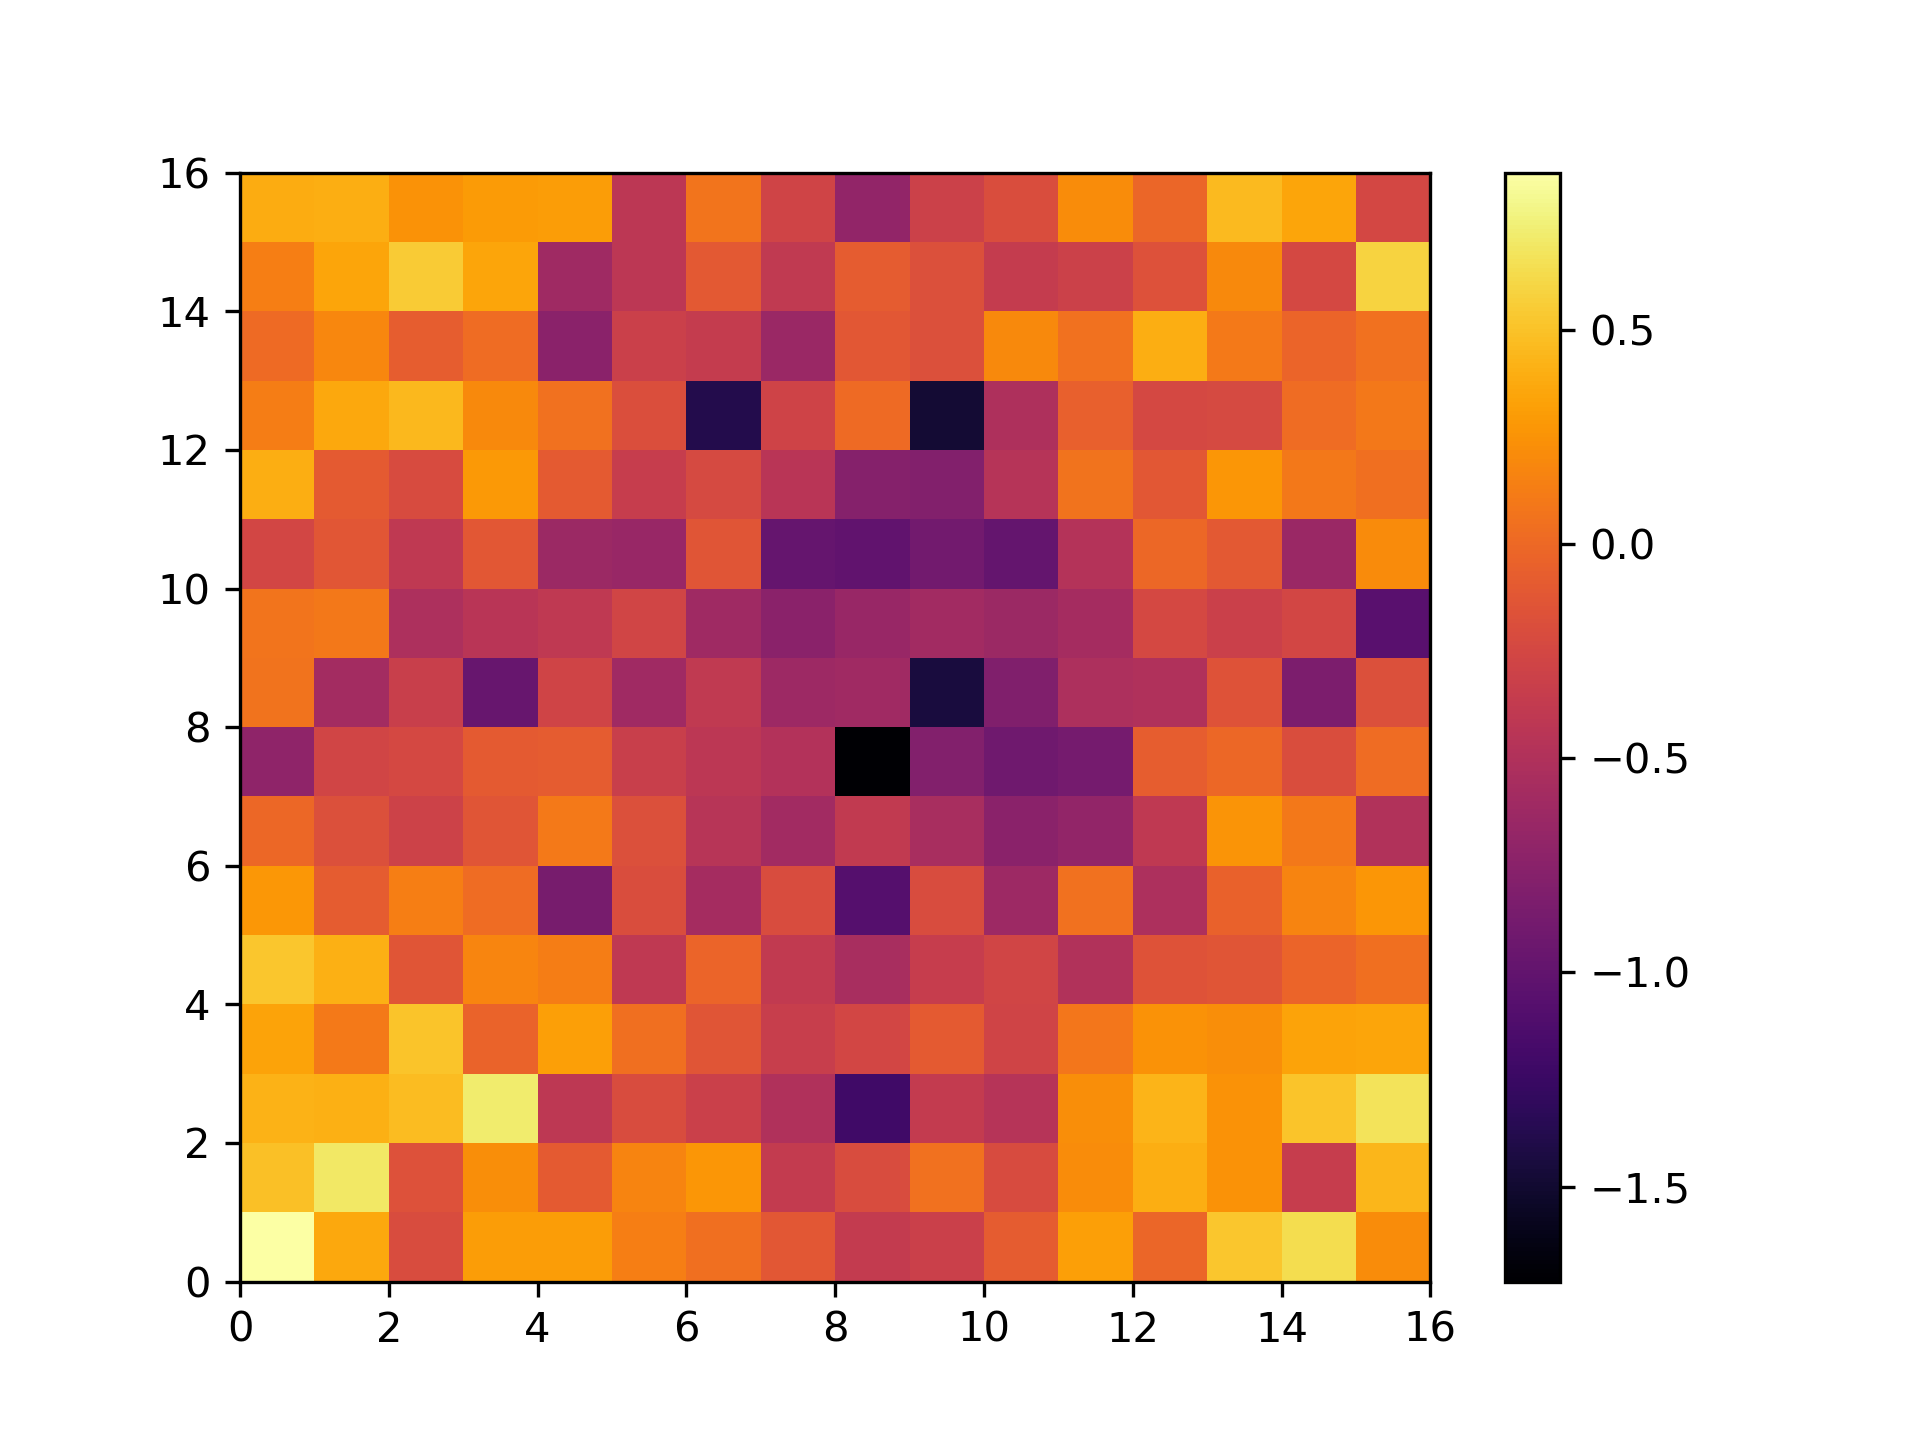
\includegraphics[width=.8\linewidth]{./plots/fourier_11.5.png}
  \caption{A 2D slice of the logarithm of the absolute value of the Fourier-transformed potential at z=11.5}
  \label{fig:four_11}
\end{figure}

\begin{figure}[H]
  \centering
  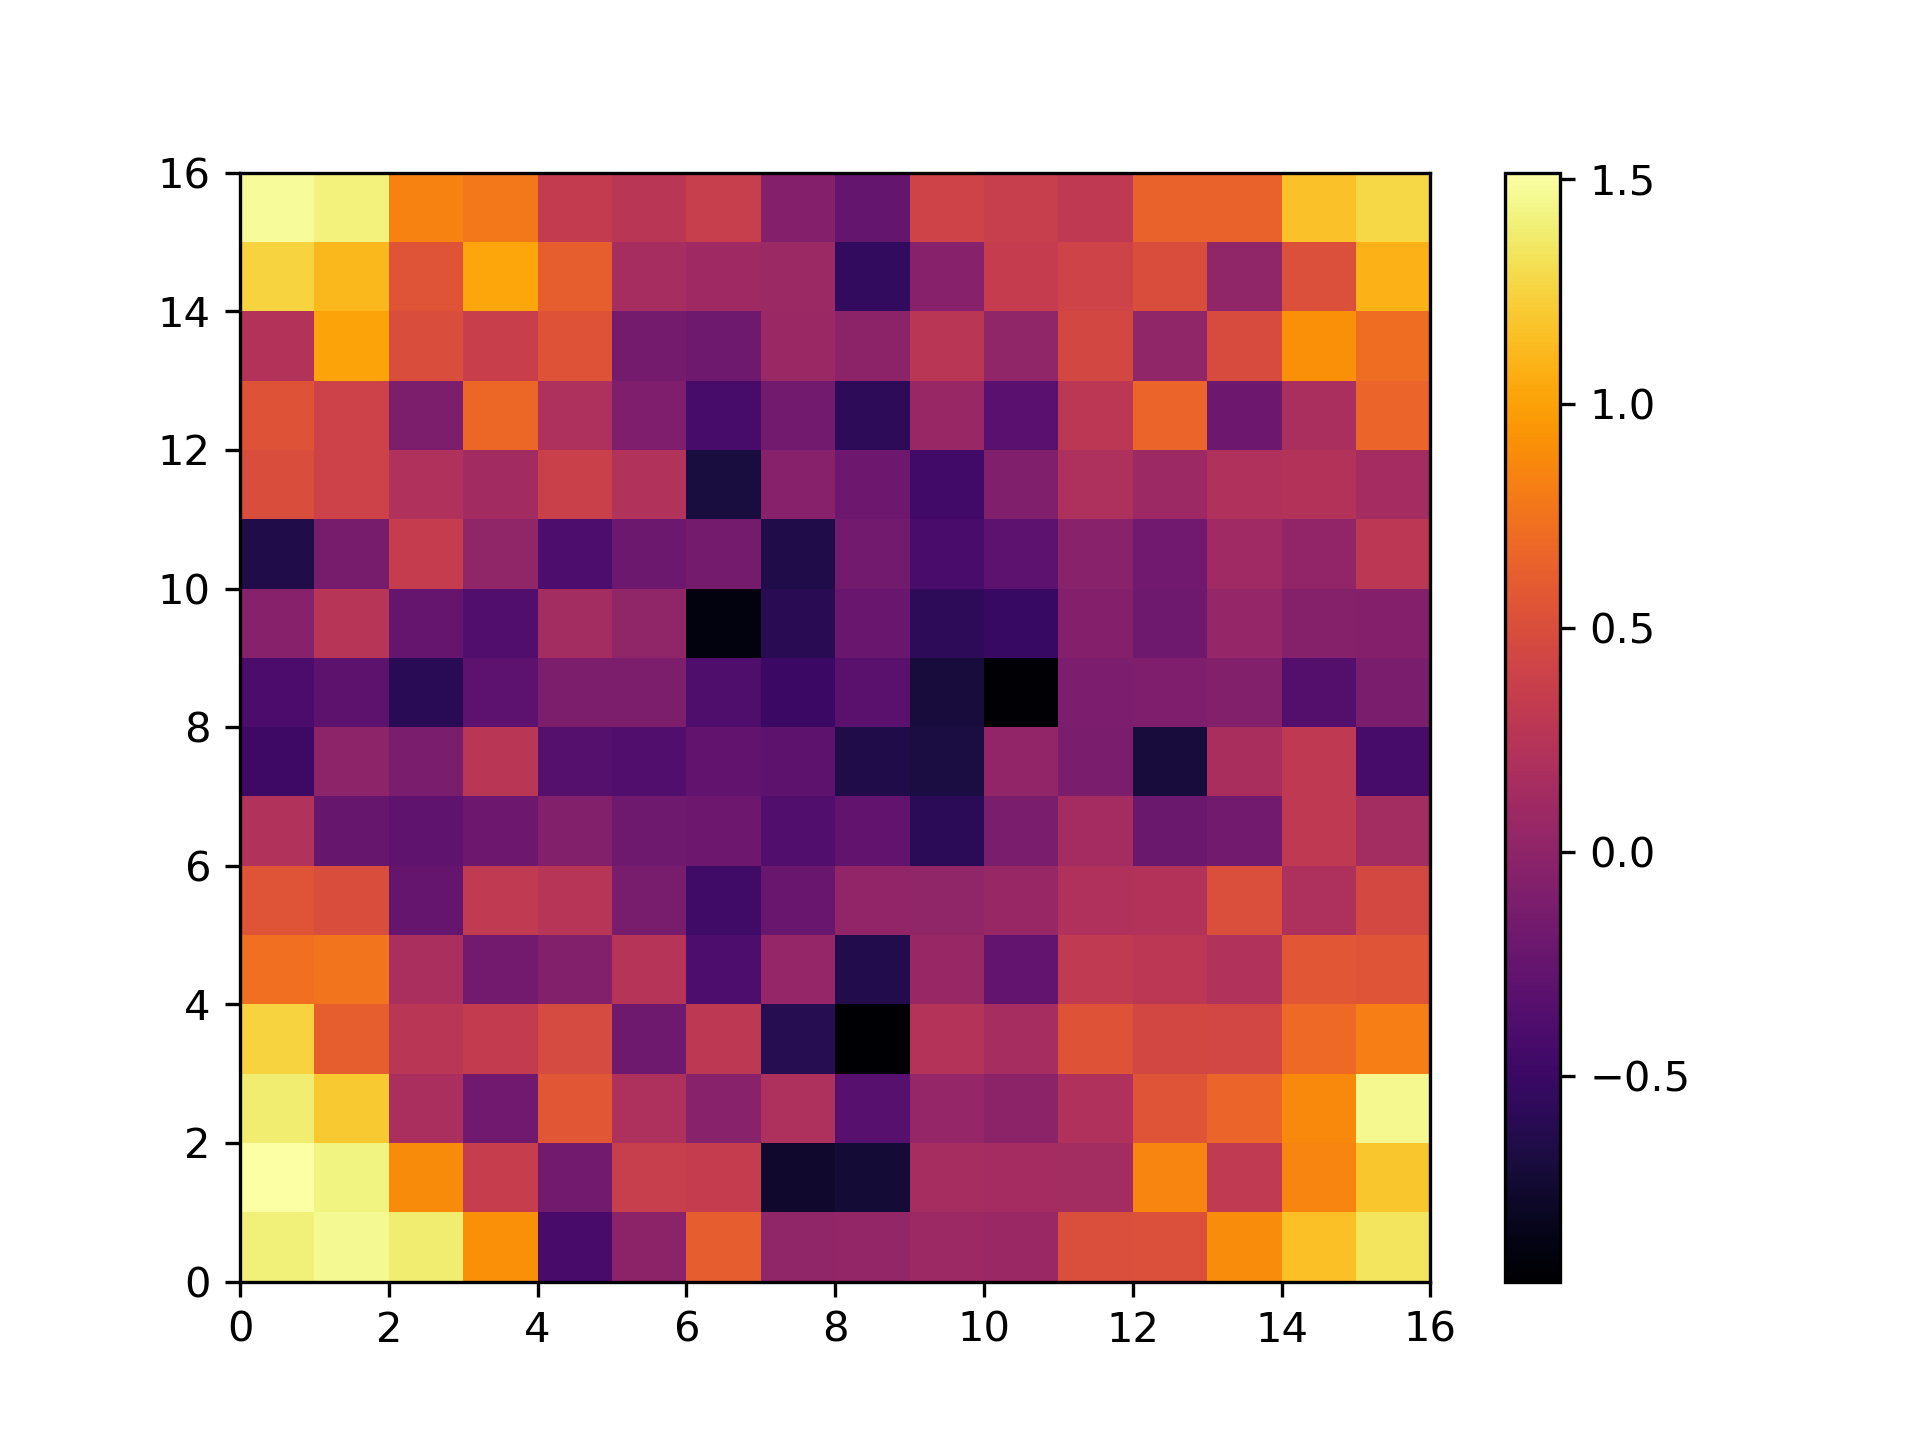
\includegraphics[width=.8\linewidth]{./plots/fourier_14.5.png}
  \caption{A 2D slice of the logarithm of the absolute value of the Fourier-transformed potential at z=14.5}
  \label{fig:four_14}
\end{figure}

As we can see our results for the potential (\Cref{fig:for_4,fig:for_9,fig:for_11,fig:for_14}) make intuitive sense when we compare them with the density slices in \Cref{fig:2d_4,fig:2d_9,fig:2d_11,fig:2d_14}. We see that high-density regions lead to a smaller gravitational potential because we used the minus sign in \Cref{eq:four_pot}. We use an inverse colormap to highlight those regions. 

\begin{figure}[H]
  \centering
  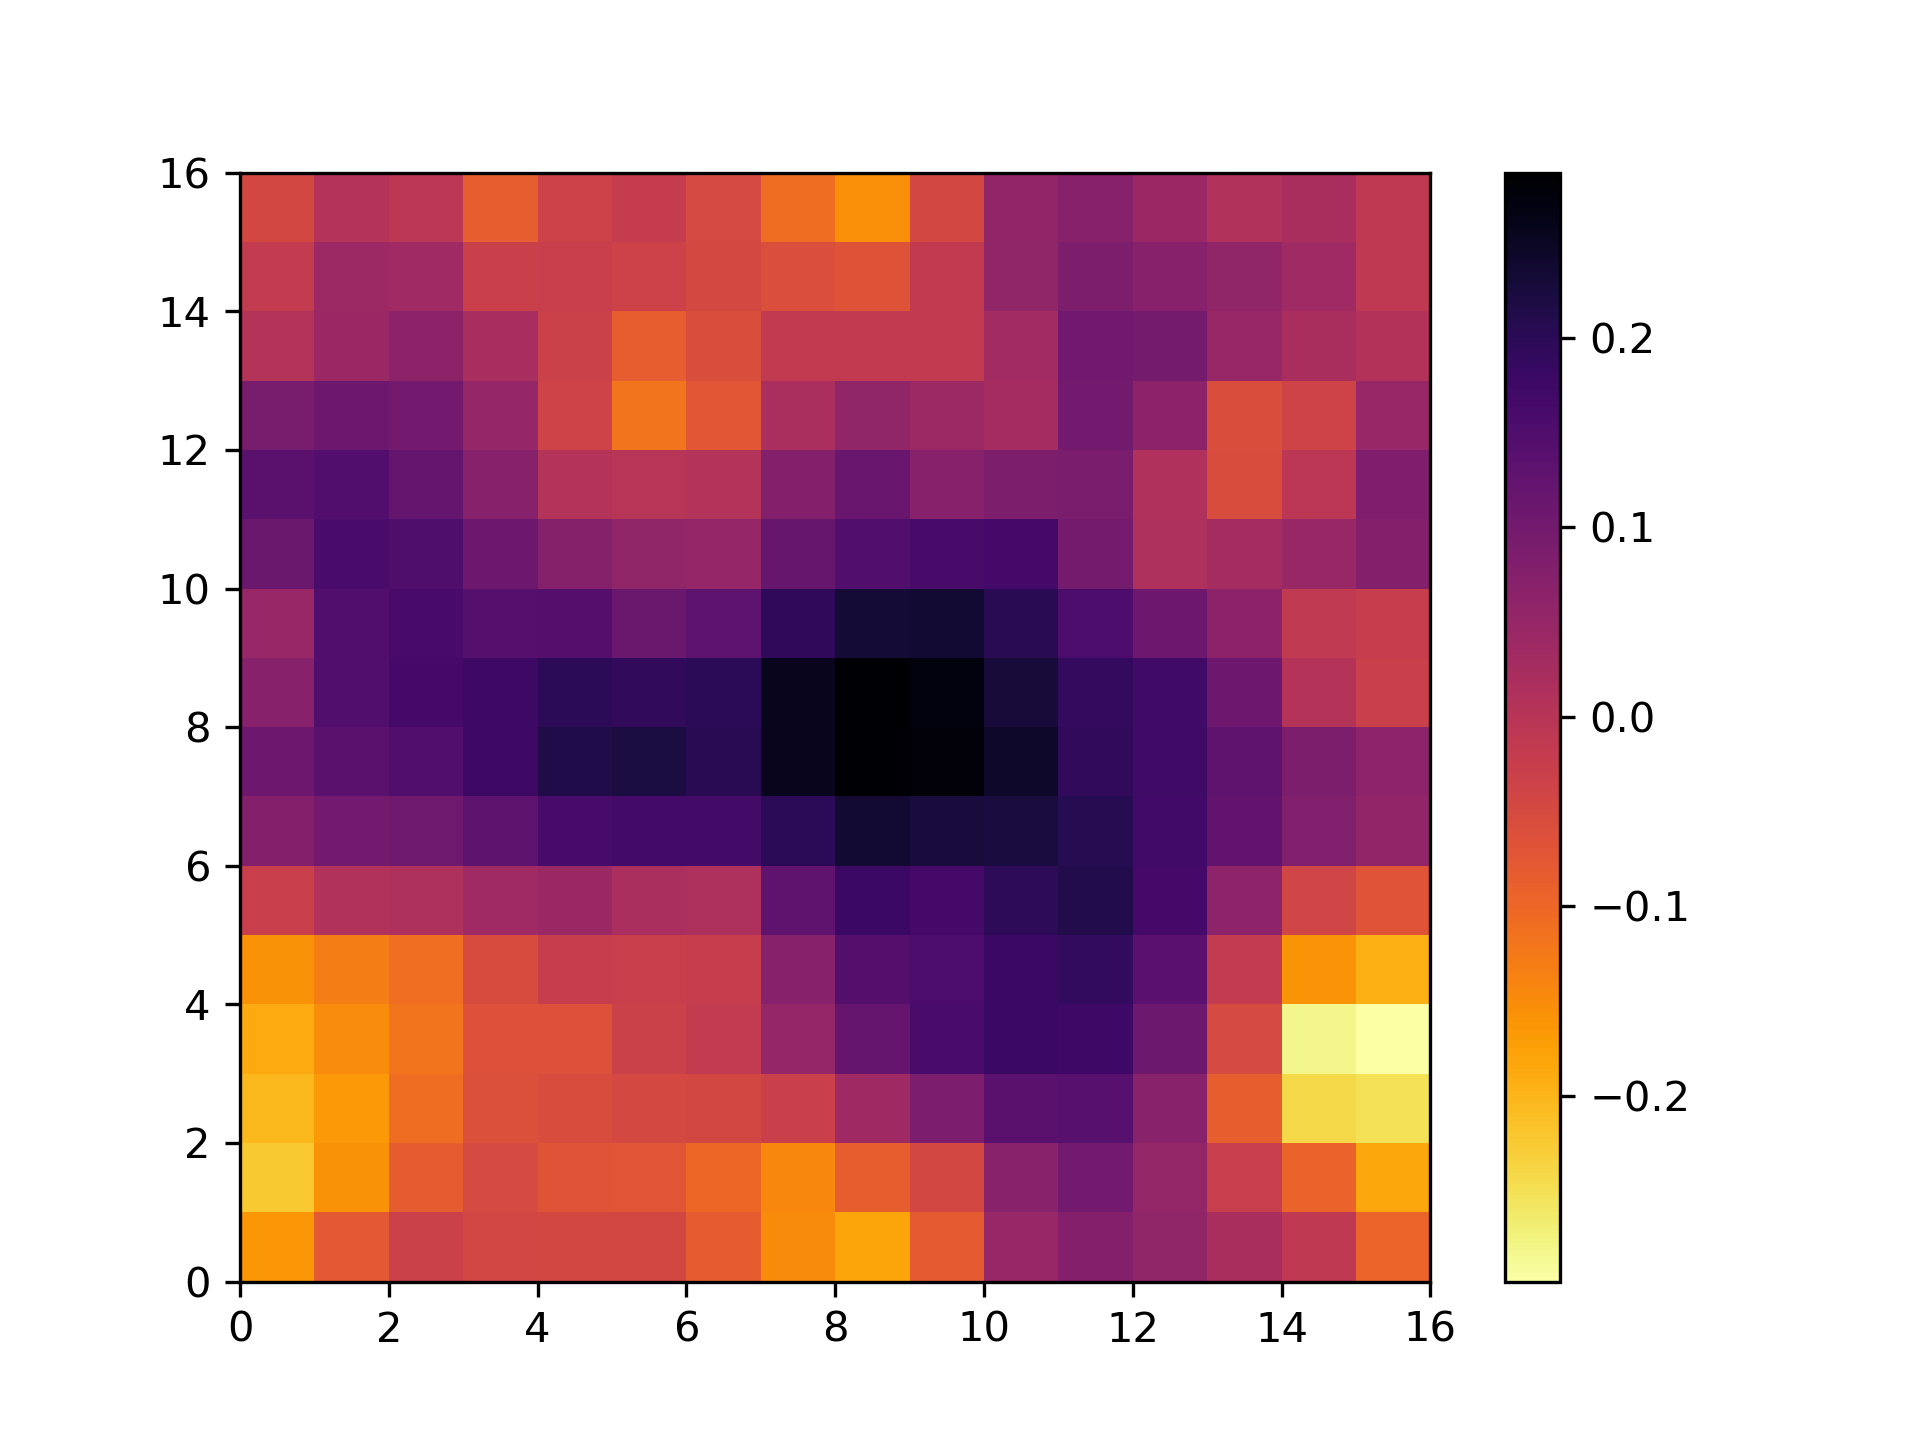
\includegraphics[width=.8\linewidth]{./plots/potential_4.5.png}
  \caption{A 2D slice of the potential at z=4.5}
  \label{fig:for_4}
\end{figure}

\begin{figure}[H]
  \centering
  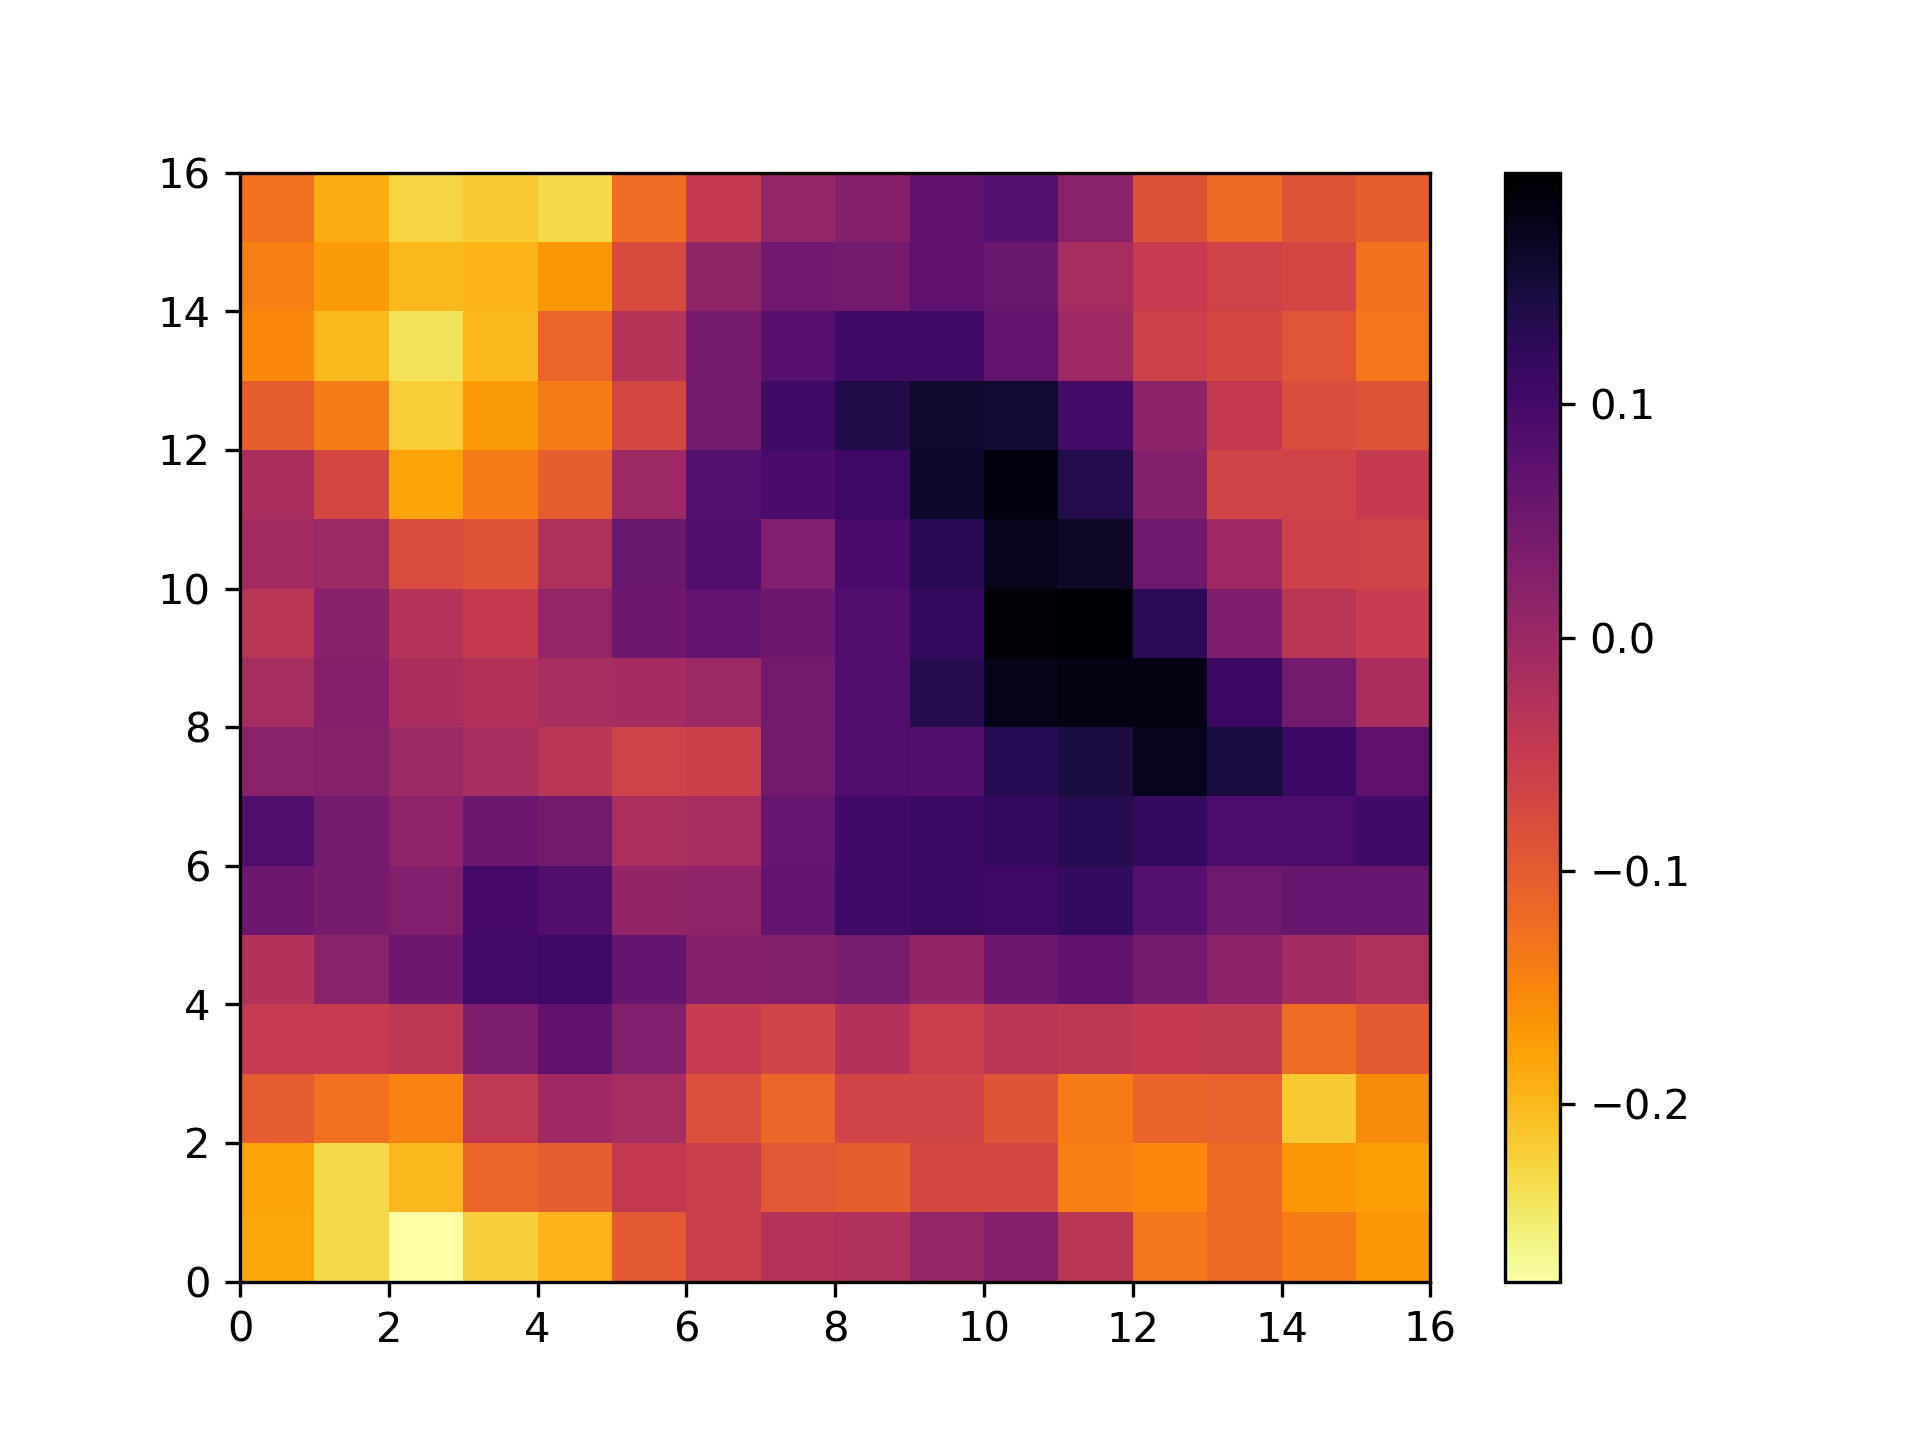
\includegraphics[width=.8\linewidth]{./plots/potential_9.5.png}
  \caption{A 2D slice of the potential at z=9.5}
  \label{fig:for_9}
\end{figure}

\begin{figure}[H]
  \centering
  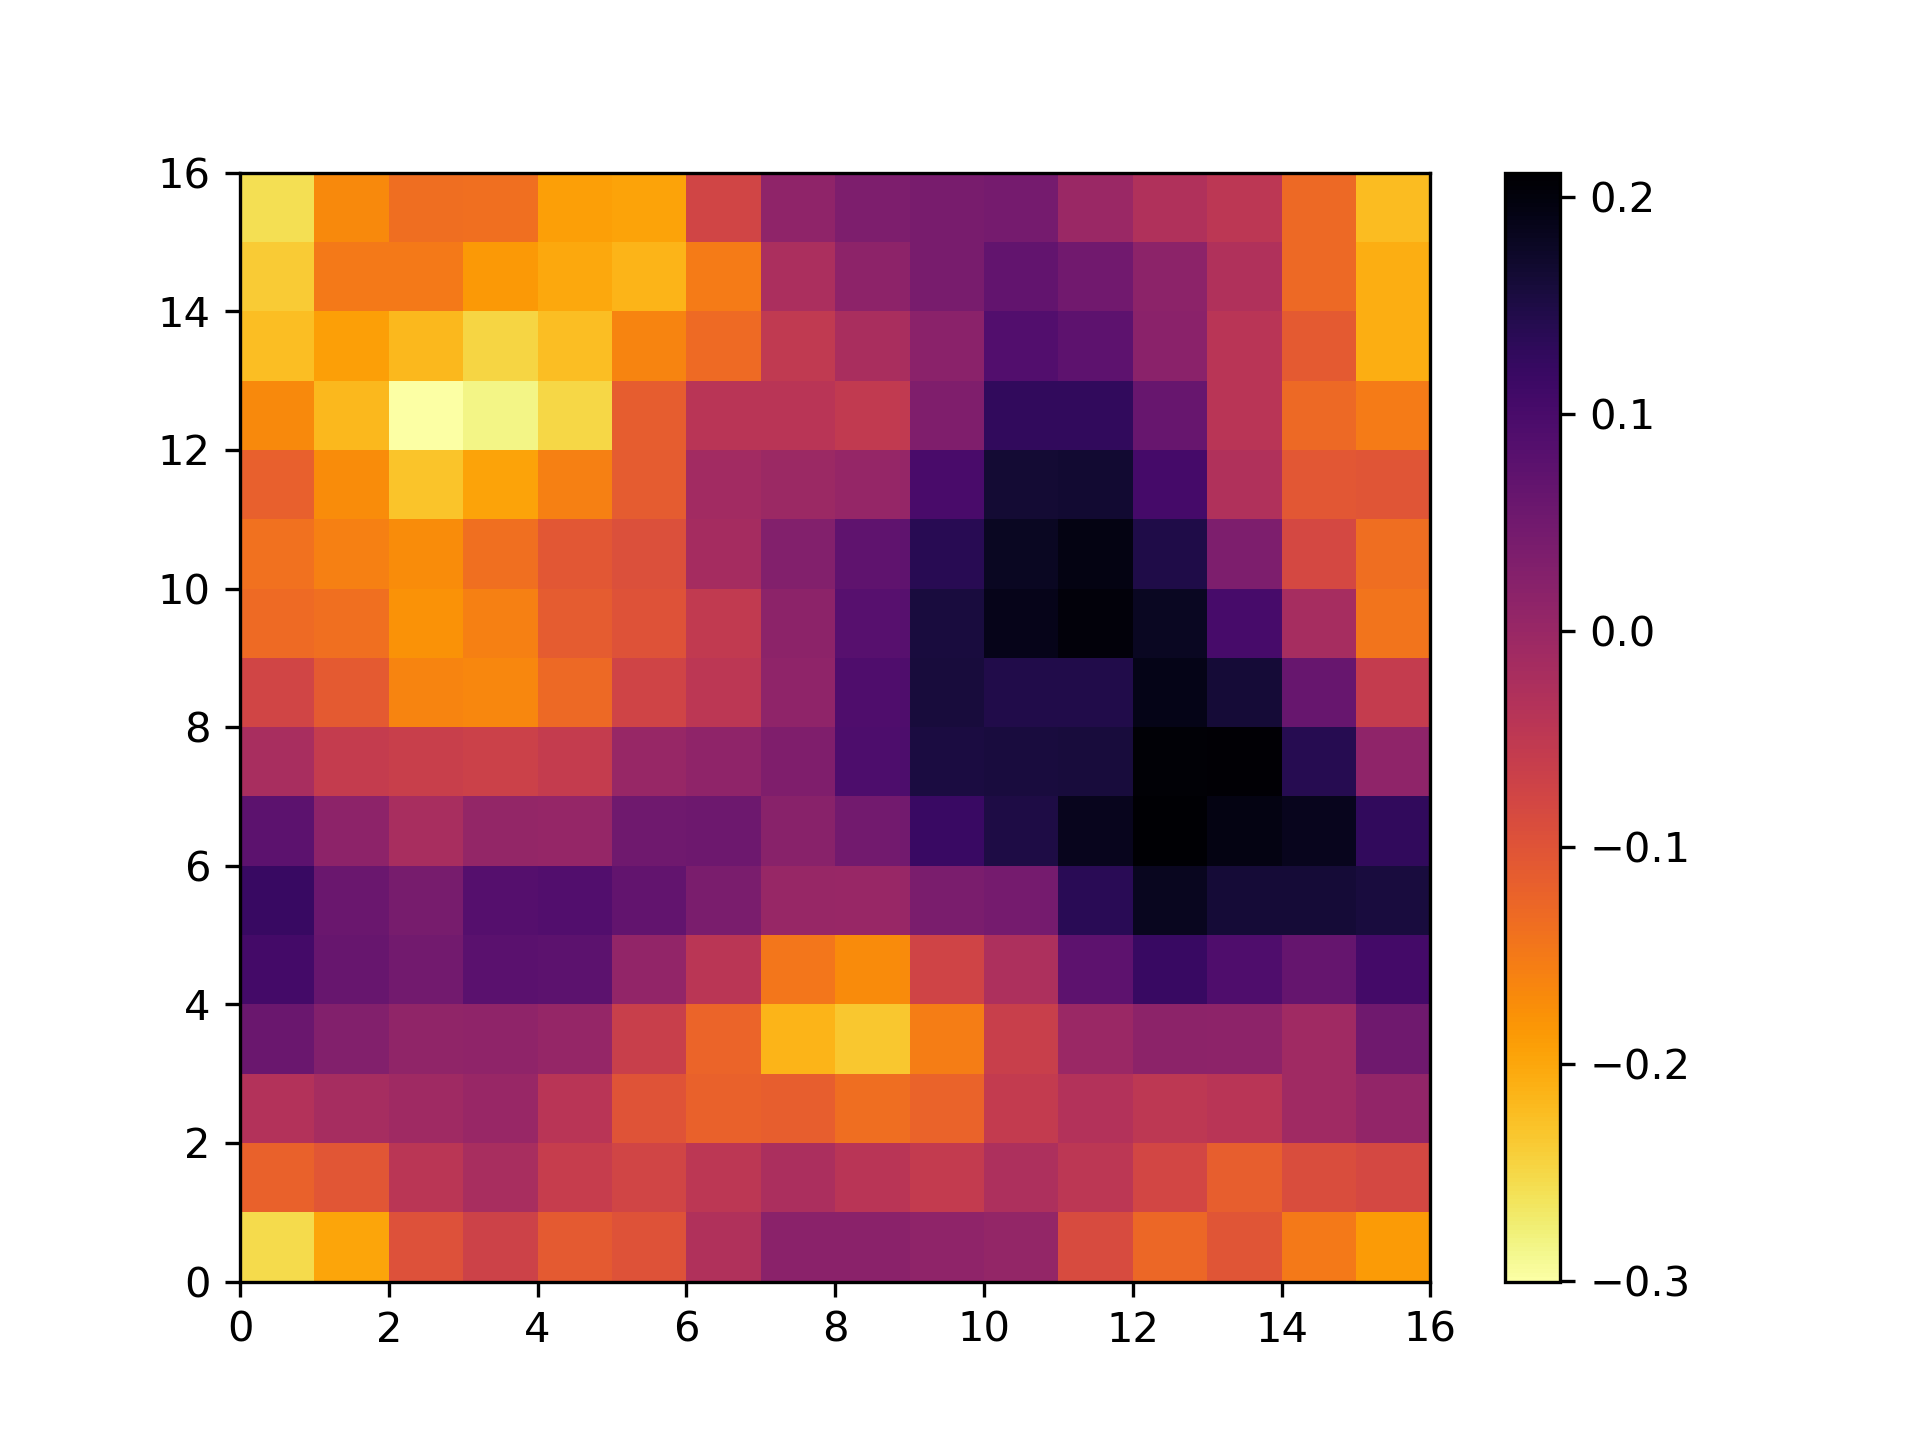
\includegraphics[width=.8\linewidth]{./plots/potential_11.5.png}
  \caption{A 2D slice of the potential at z=11.5}
  \label{fig:for_11}
\end{figure}

\begin{figure}[H]
  \centering
  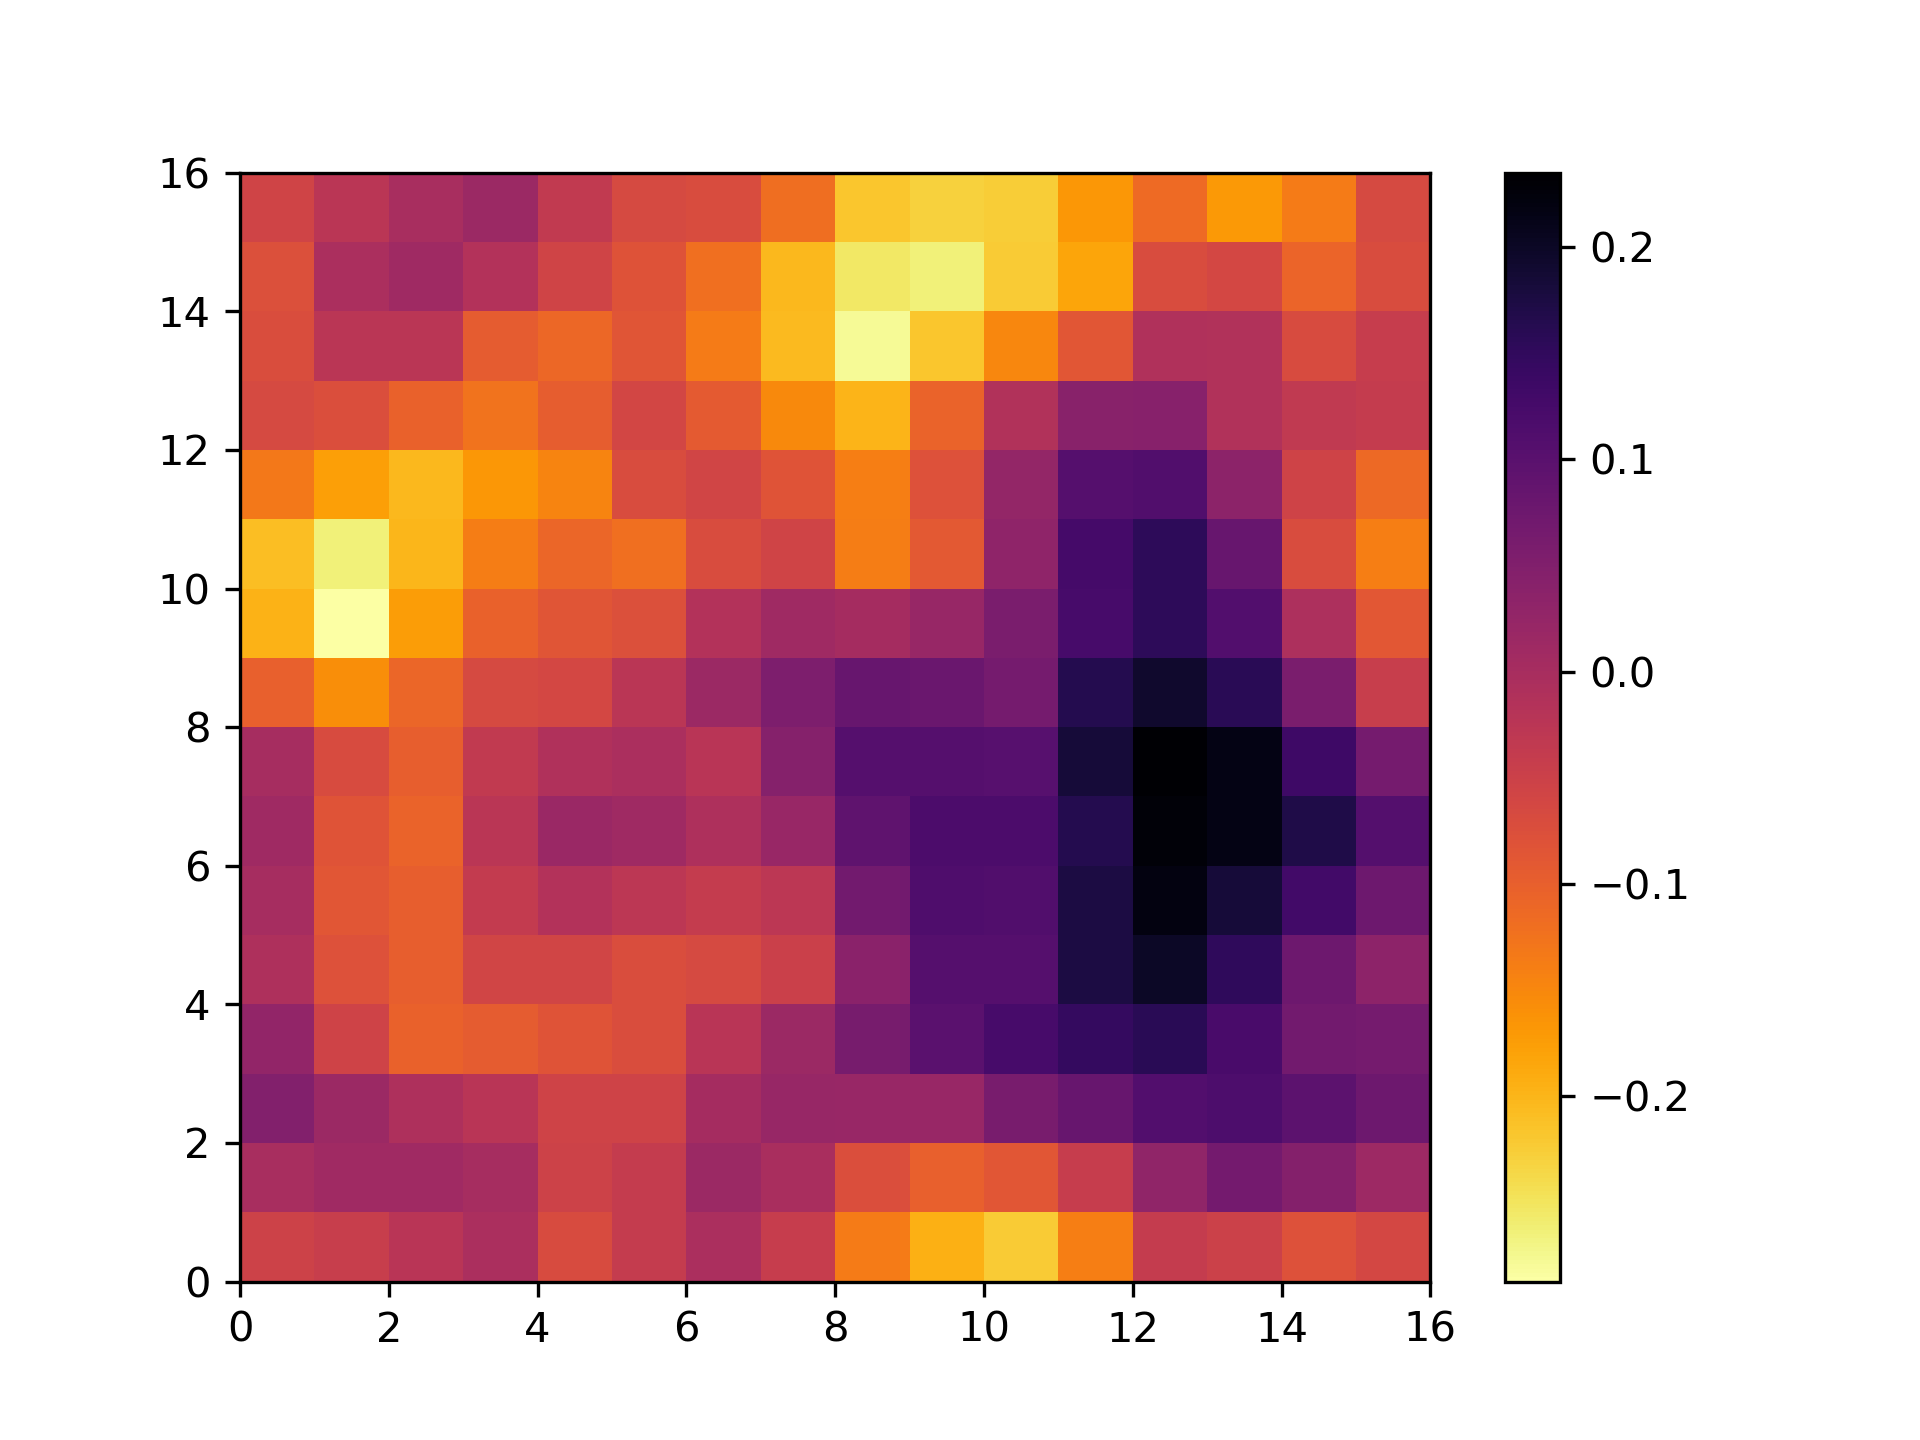
\includegraphics[width=.8\linewidth]{./plots/potential_14.5.png}
  \caption{A 2D slice of the potential at z=14.5}
  \label{fig:for_14}
\end{figure}


\section{Spiral and elliptical galaxies}

In this section, we will use Logistic Regression to classify galaxies in either spirals or ellipticals using different sets of features.

\subsection{Preparing the dataset}
\label{sec:prep}

Our dataset contains 5 columns. The last column consists of the labels with a flag that indicates whether it is a spiral (1) or elliptical (0). The first four columns contain different parameters of each galaxy. First, we have a parameter indicating how much the galaxy is dominated by ordered rotation, then an estimate of their color followed by a measure of how extended each galaxy is, and lastly the flux of an emission line used to measure the star formation rate of galaxies. 

To prepare the dataset we want to create an input array with shape $[m \times n]$ where $m$ is the length of the dataset and $n$ is the number of features (in our case 4). We want to normalize each feature to have a mean of 0 and a standard deviation of 1. We do that with the following formula:
\begin{equation}
  x \leftarrow \frac{x-\mathrm{mean}(x)}{\mathrm{std}(x)}
\end{equation} 

\lstinputlisting{prepare.py}

We save the input array and we show the first 10 lines of the text file. We also create histogram plots of the 4 distributions in \Cref{fig:distr_1,fig:distr_2,fig:distr_3,fig:distr_4}. We use a logarithmic scale to better indicate the outliers and regions with small values of $N$.

\lstinputlisting[firstline=0,lastline=10]{output/input.txt}

\begin{figure}[H]
  \centering
  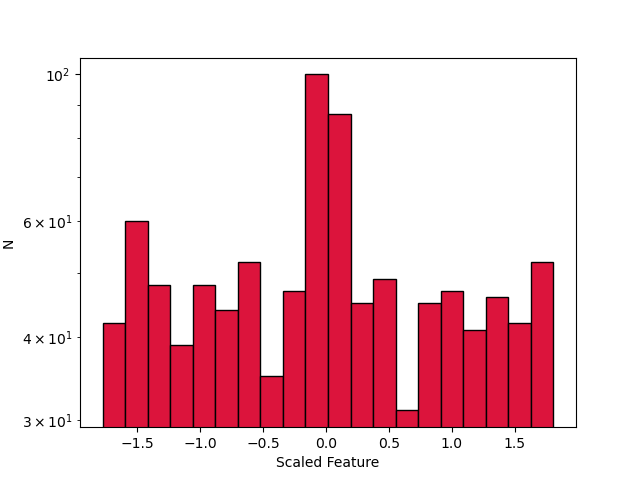
\includegraphics[width=.7\linewidth]{./plots/distr_0.png}
  \caption{The distribution of the 1st column after applying feature scaling.}
  \label{fig:distr_1}
\end{figure}

\begin{figure}[H]
  \centering
  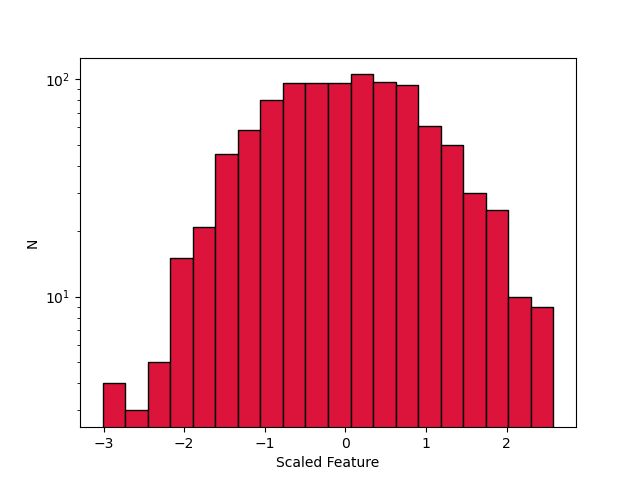
\includegraphics[width=.7\linewidth]{./plots/distr_1.png}
  \caption{The distribution of the 2nd column after applying feature scaling.}
  \label{fig:distr_2}
\end{figure}

\begin{figure}[H]
  \centering
  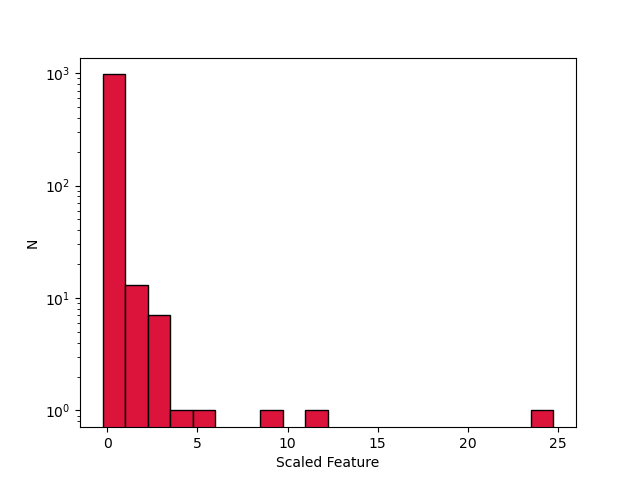
\includegraphics[width=.7\linewidth]{./plots/distr_2.png}
  \caption{The distribution of the 3rd column after applying feature scaling.}
  \label{fig:distr_3}
\end{figure}

\begin{figure}[H]
  \centering
  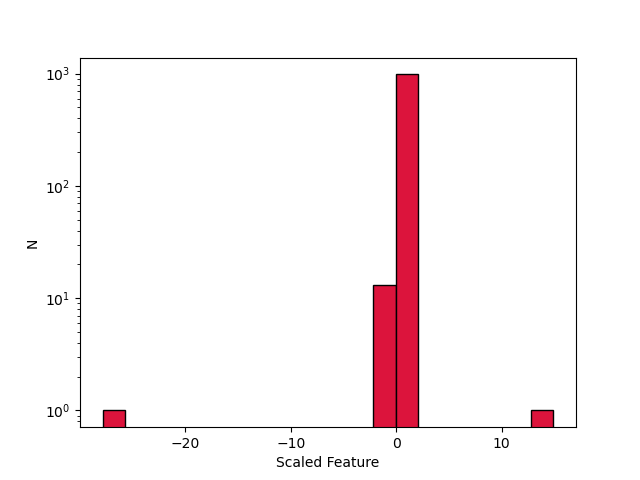
\includegraphics[width=.7\linewidth]{./plots/distr_3.png}
  \caption{The distribution of the 4th column after applying feature scaling.}
  \label{fig:distr_4}
\end{figure}

\subsection{Logistic Regression}

We now want to perform a Logistic Regression to classify the galaxies in spirals and ellipticals. The first step is to have a minimization algorithm to find the best weights. We use the ``bfgs'' function that utilizes the Quasi-Newton method of BFGS. The implementation that we used follows the pseudocode and equations from \shortciteA{book1} (pages 136-140). For the line minimization that is required, we use the ``golden\_search'' function that utilizes the golden search algorithm for function minimization. The implementation is the same as we did in previous assignments with minor changes for compatibility with ``bfgs''.

Now that we have our minimization routine we will do the logistic regression. We define the ``sigmoid'' function to calculate the sigmoid and define the loss function of the logistic regression in ``loss\_fun'':
\begin{equation}
  J(\theta) = -y \log(sig(X \cdot \theta)) - (1-y) \log(1-sig(X \cdot \theta))
\end{equation}
where $X$ is the input, $\theta$ are the model parameters and $y$ the true labels. We also define the gradient of the loss function in ``grad\_loss'':
\begin{equation}
  J'(\theta) = \frac{1}{m} X^T \cdot [sig(X \cdot \theta)-y]
\end{equation}

In the ``fit'' function we perform the training of our model by initializing the weights at 1 and then using the minimization function to find the best values for the weights by minimizing the loss function. We also define a function for the plotting of the loss function. 

\lstinputlisting{classification.py}

In the main part of the script, we load the data, using the rescaled features we calculated before. We then perform the fitting for all possible combinations of different features. In \Cref{fig:train} we can see the value of the loss function during the training. As we can see including different features is allowing us to reach even lower values. 

The different distinct groups that appear in \Cref{fig:train} are because of the different combinations of features. The best performance is when we include the 1st and 2nd features. The worst performance is when neither is present. Including the 1st without the 2nd lead to better performance than the opposite. The reason these two features give such a performance improvement is that they have a better distribution as was seen in \Cref{sec:prep}, and they are also better indicators of whether a galaxy is spiral or elliptical.

\begin{figure}[H]
  \centering
  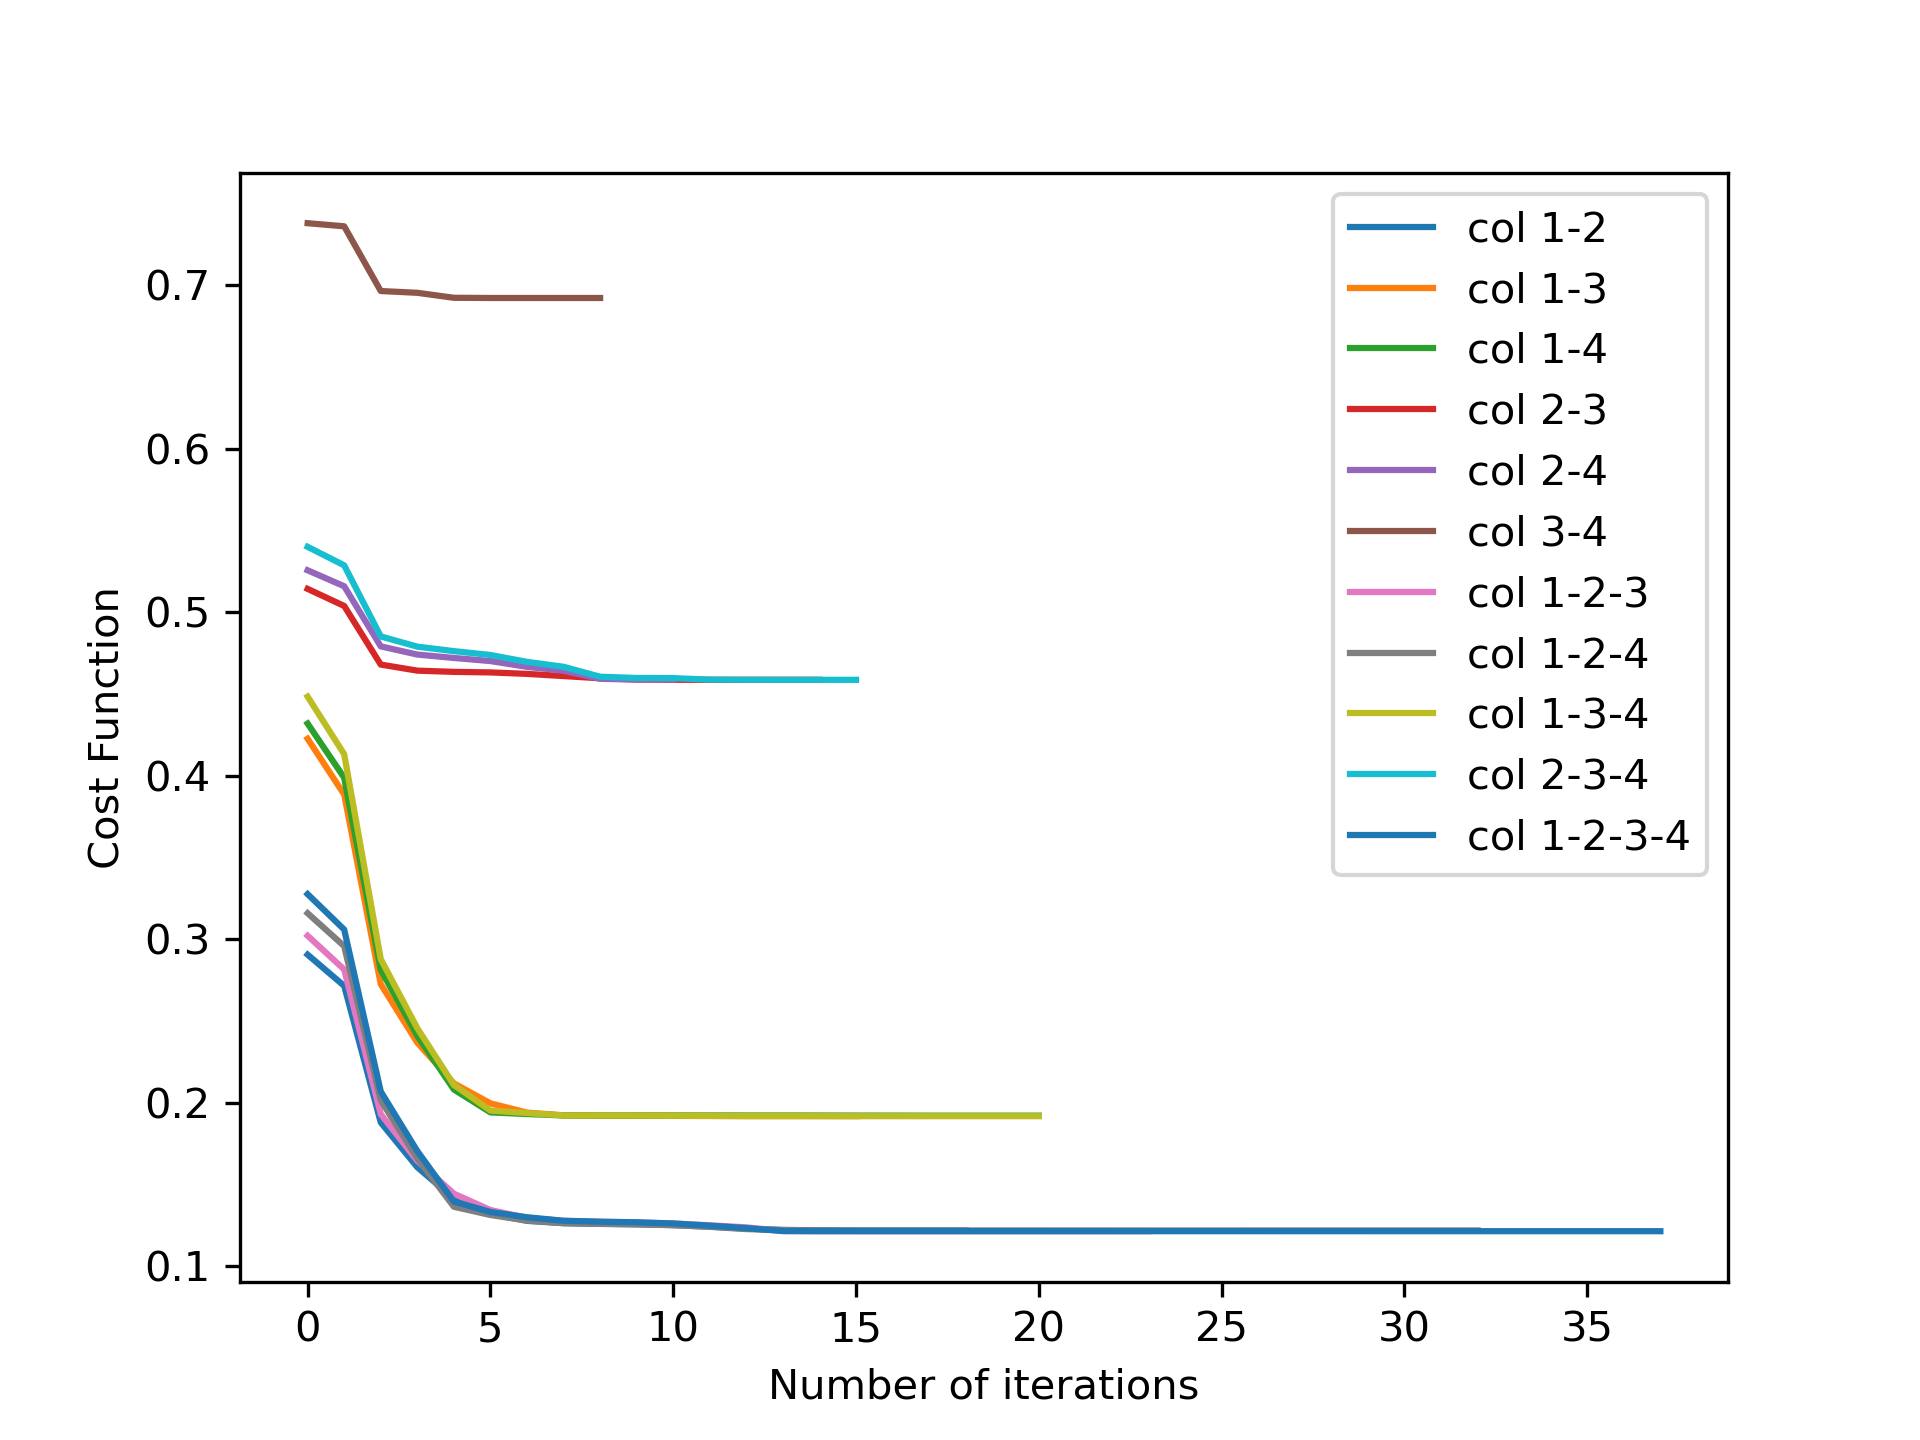
\includegraphics[width=.7\linewidth]{./plots/training.png}
  \caption{}
  \label{fig:train}
\end{figure}

\subsection{Evaluate}

We now want to evaluate our models. We create the ``predict'' function to generate predictions with the weights of our model and the input features. We define the ``evaluate'' function that utilizes the predictions to calculate the number of
true/false positives/negatives. The ``f\_score'' function calculates the $F_{\beta}$ value. We then create two functions to plot two features against each other with the decision boundary. 

\lstinputlisting{evaluation.py}

In the main part of the script, we load the data and the weights we calculated in the previous script. We go again for each possible combination of features and calculate the true/false positives/negatives of the model. We also calculate accuracy and the $F_1$ score. For the combinations of 2 features, we also plot them with the decision boundary.

\lstinputlisting{output/evaluation.txt}

As we can see our results confirm the ones we got in \Cref{fig:train}. The combinations that include the first two columns give an accuracy and $F_1$ score of 0.948 meaning that out of 1000 cases, only 52 were mislabeled. Other combinations vary in performance. The worst performance comes for the combination of the 3rd and 4th columns which as we already mentioned doesn't include either the 1st or 2nd column and is unable to distinguish between the two having an accuracy of less than 0.5 and a very low $F_1$ score. 

In \Cref{fig:boun_1_2,fig:boun_1_3,fig:boun_1_4,fig:boun_2_3,fig:boun_2_4,fig:boun_3_4} we can find the plots of each combination of features with the decision boundary. We can see how great the boundary line manages to distinguish between the spiral and elliptical galaxies in \Cref{fig:boun_1_2} where we have the first two features. The results are more mixed for the rest of them and for \Cref{fig:boun_3_4} we can see that the boundary line is unable to distinguish the galaxies, as we already mentioned that columns 3 and 4 are not able to correctly classify the galaxies by themselves. 

\begin{figure}[H]
  \centering
  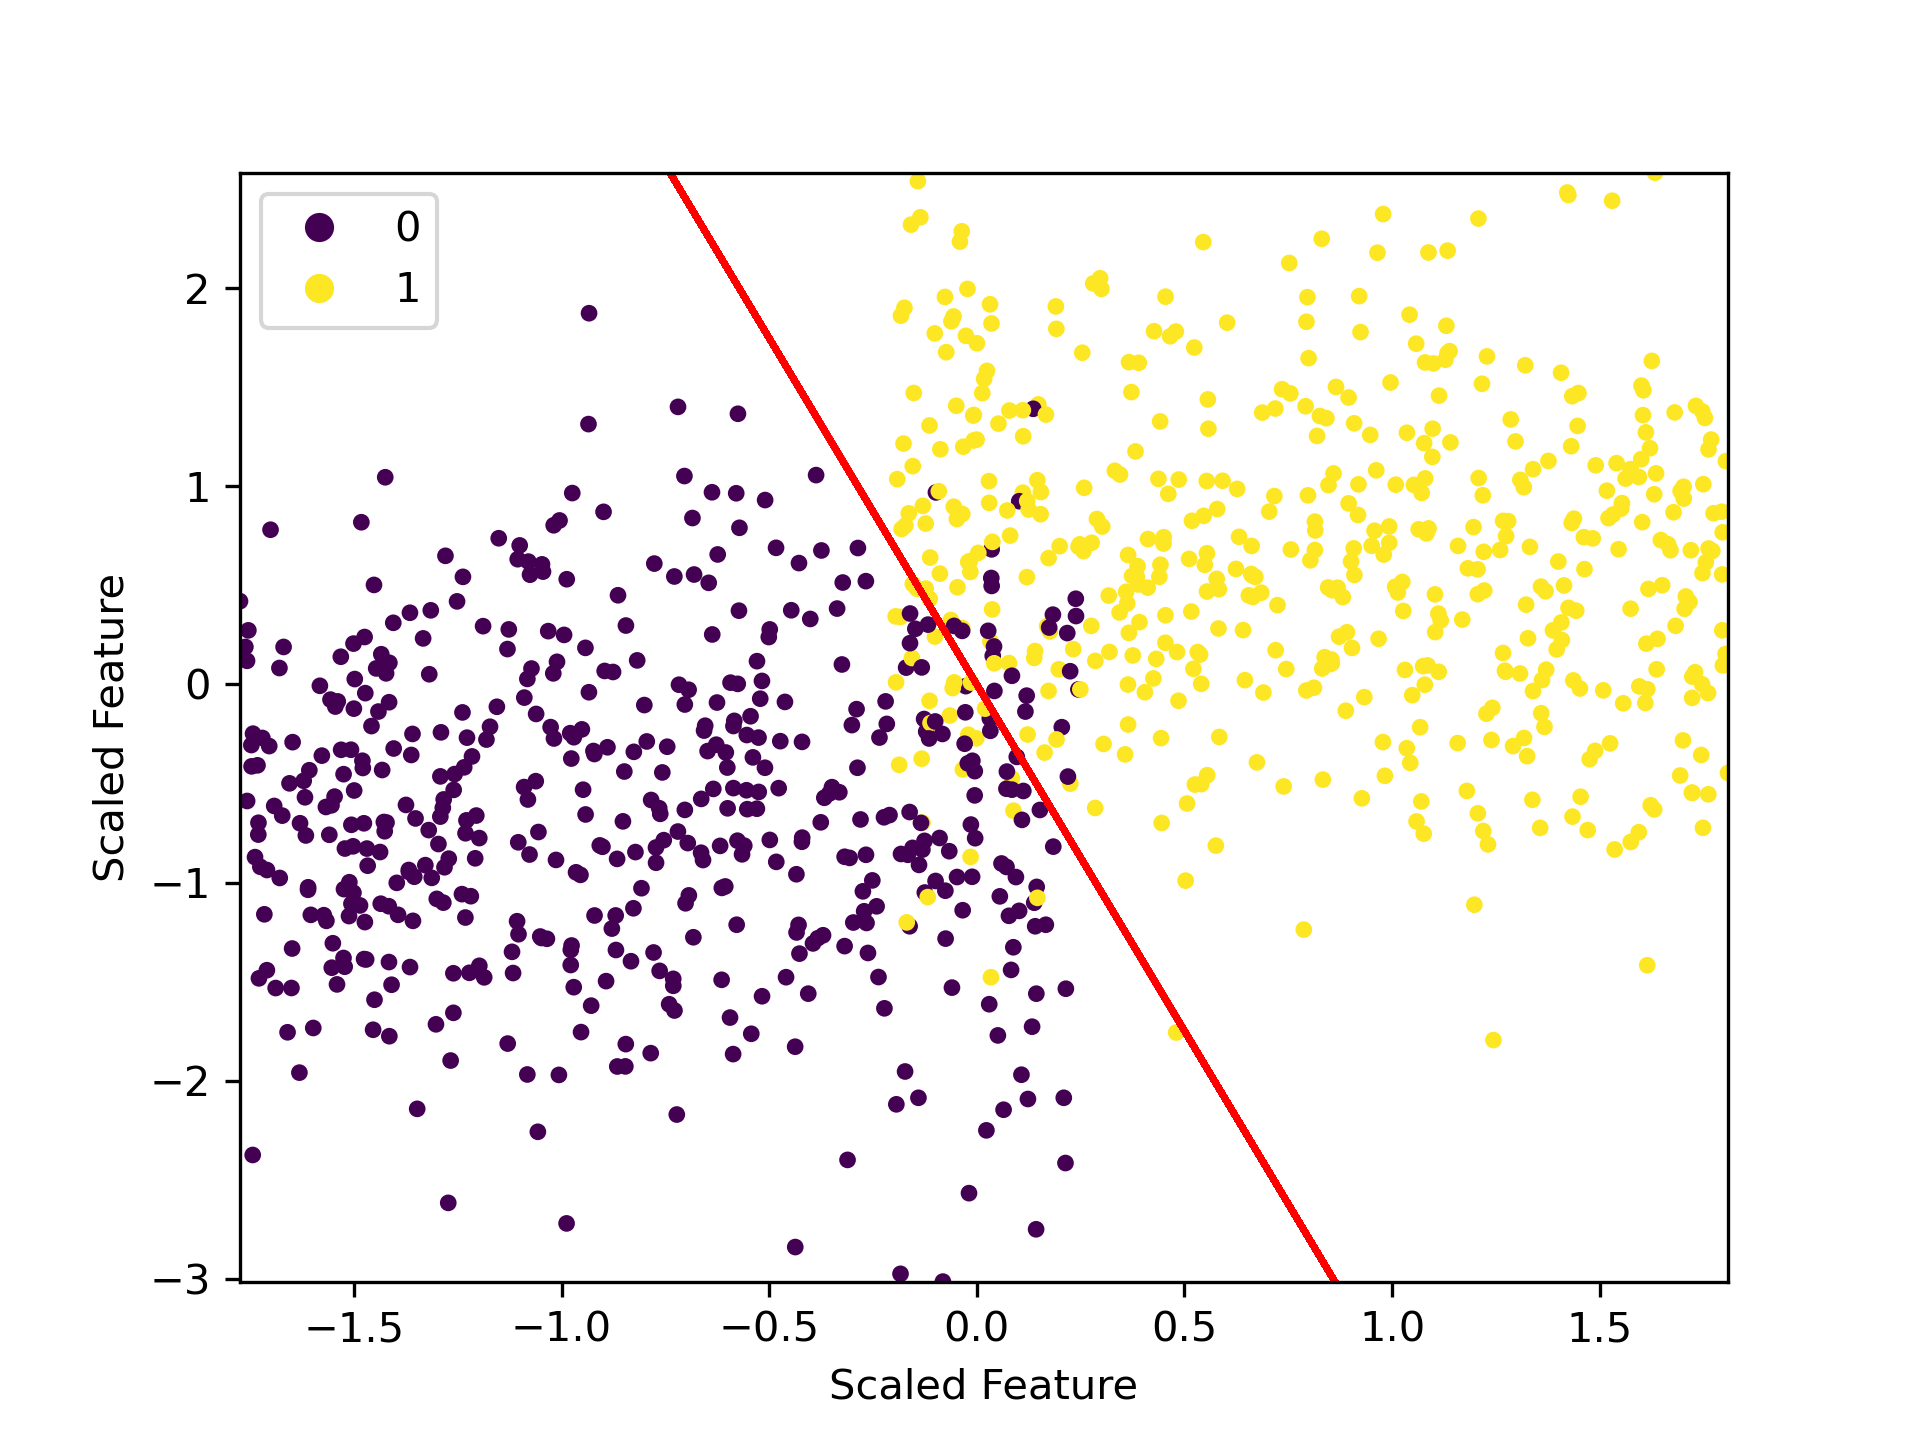
\includegraphics[width=.8\linewidth]{./plots/boundary_1-2.png}
  \caption{The 1st (x-axis) and 2nd (y-axis) rescaled features with the decision boundary. With different colors, we indicate the true labels of each point. This is the best-performing combination of features.}
  \label{fig:boun_1_2}
\end{figure}

\begin{figure}[H]
  \centering
  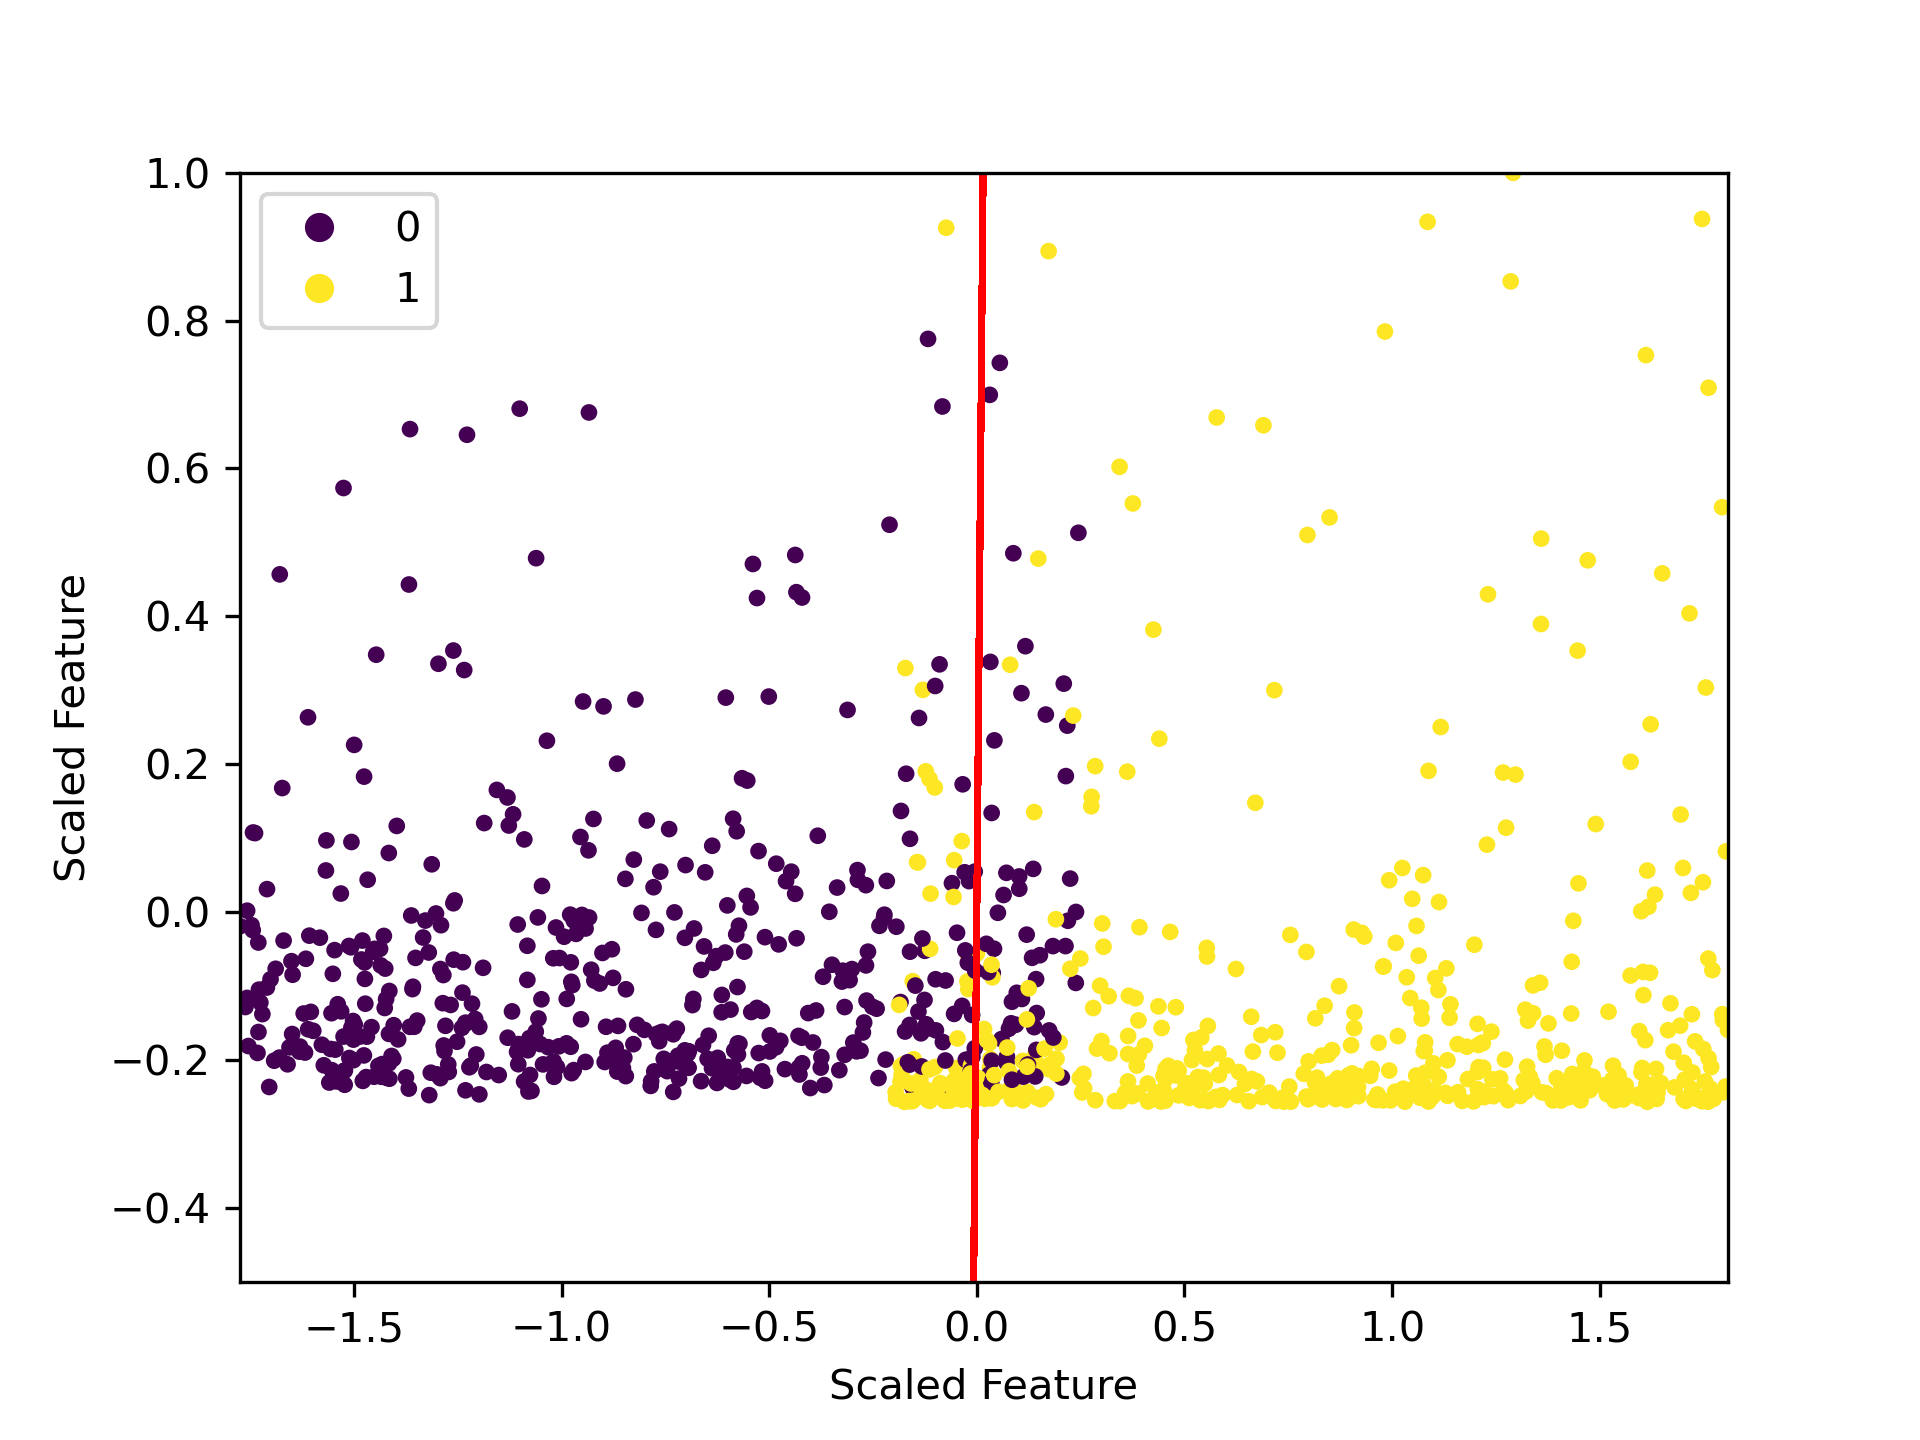
\includegraphics[width=.8\linewidth]{./plots/boundary_1-3.png}
  \caption{The 1st (x-axis) and 2nd (y-axis) rescaled features with the decision boundary. With different colors, we indicate the true labels of each point.}
  \label{fig:boun_1_3}
\end{figure}

\begin{figure}[H]
  \centering
  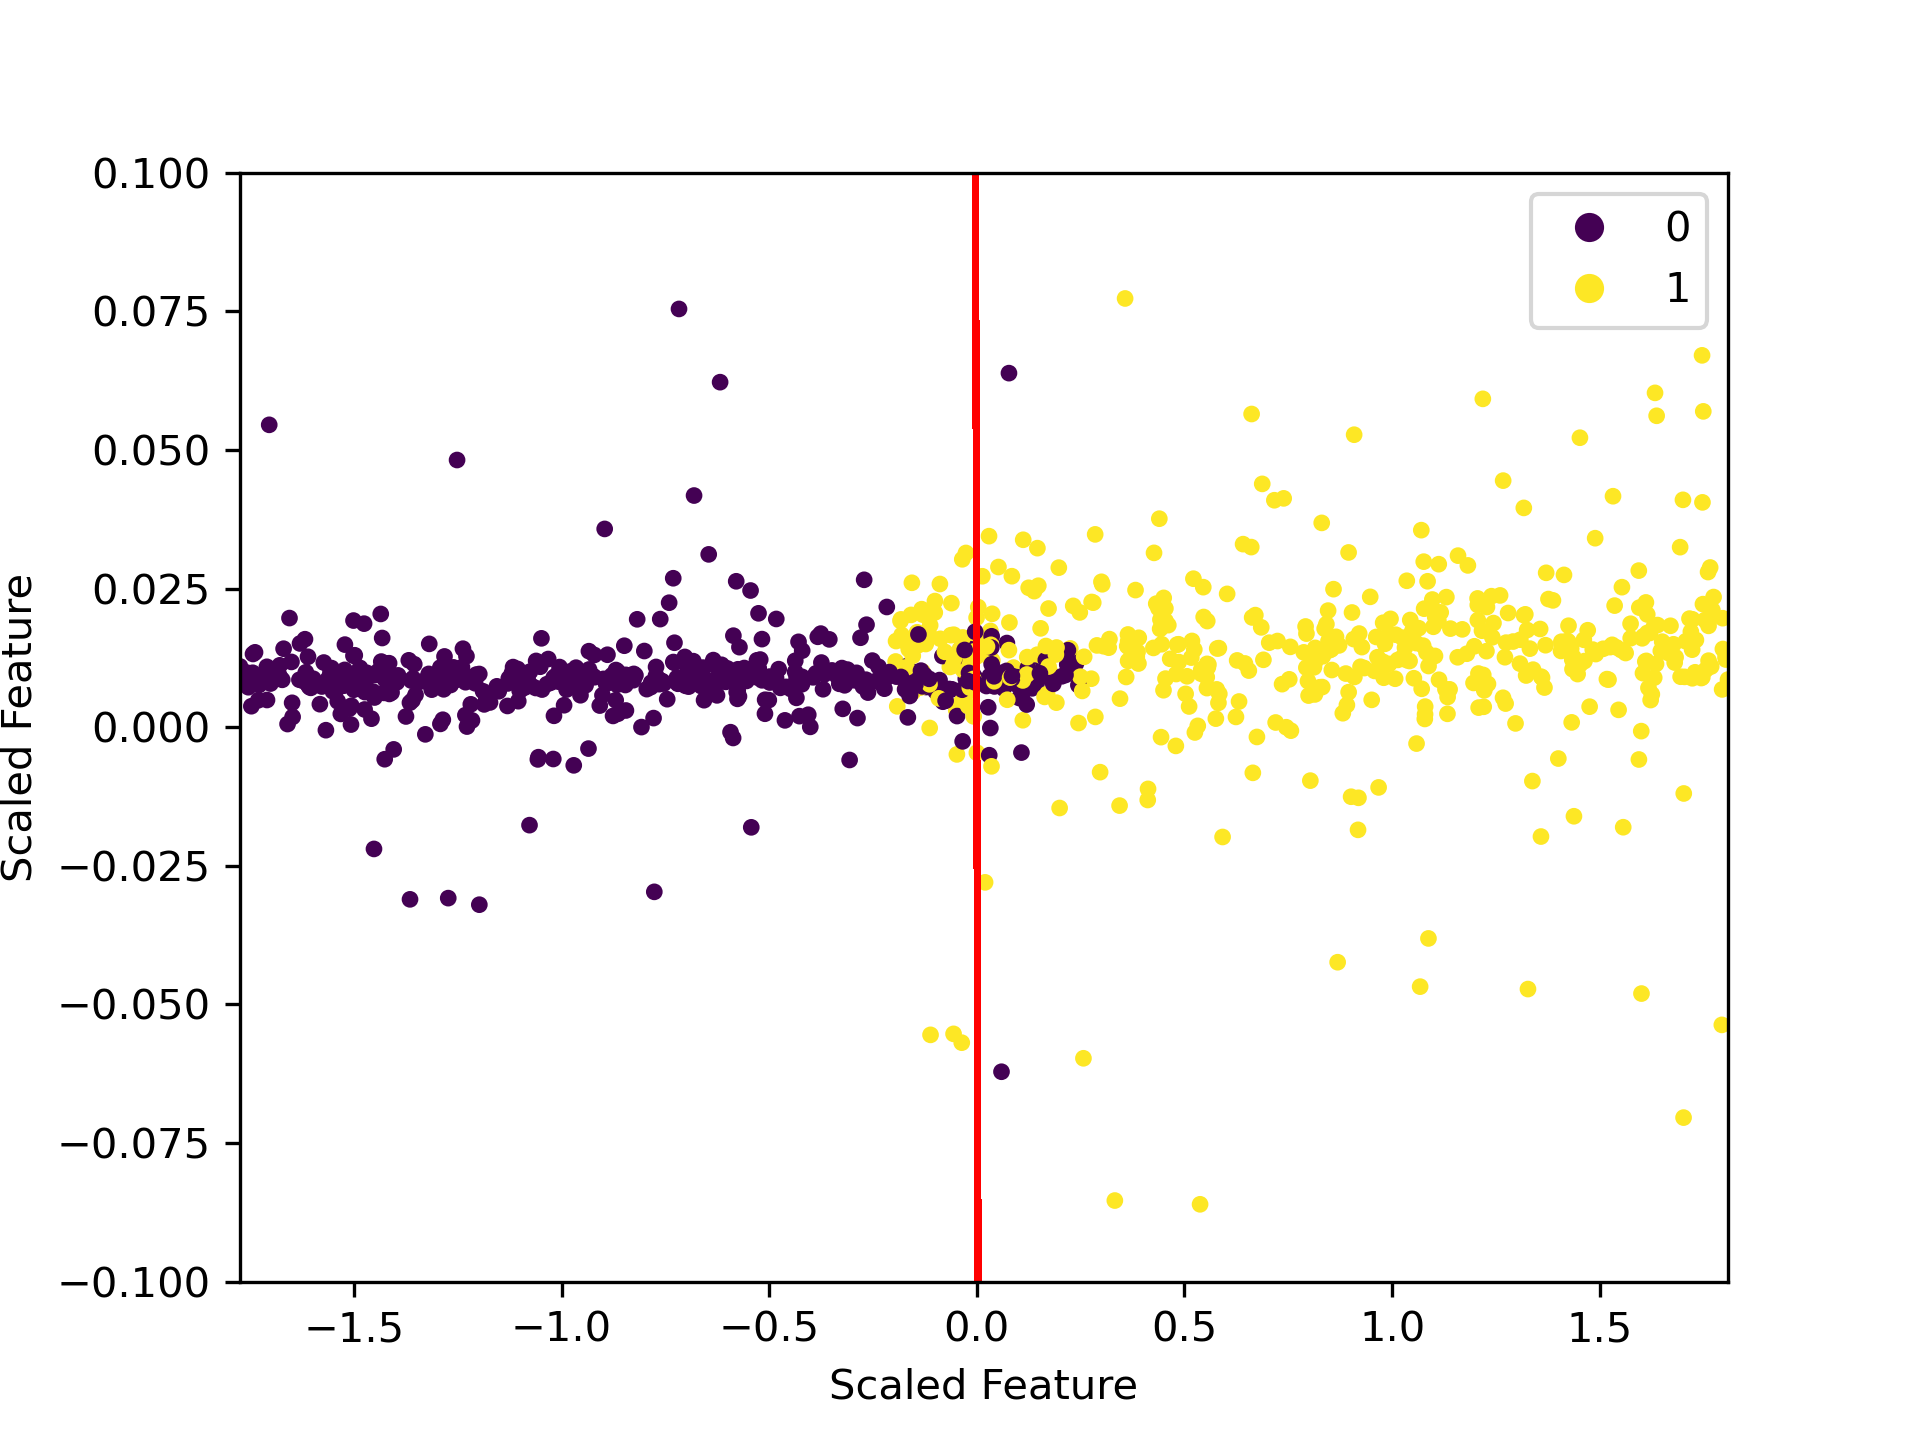
\includegraphics[width=.8\linewidth]{./plots/boundary_1-4.png}
  \caption{The 1st (x-axis) and 2nd (y-axis) rescaled features with the decision boundary. With different colors, we indicate the true labels of each point.}
  \label{fig:boun_1_4}
\end{figure}

\begin{figure}[H]
  \centering
  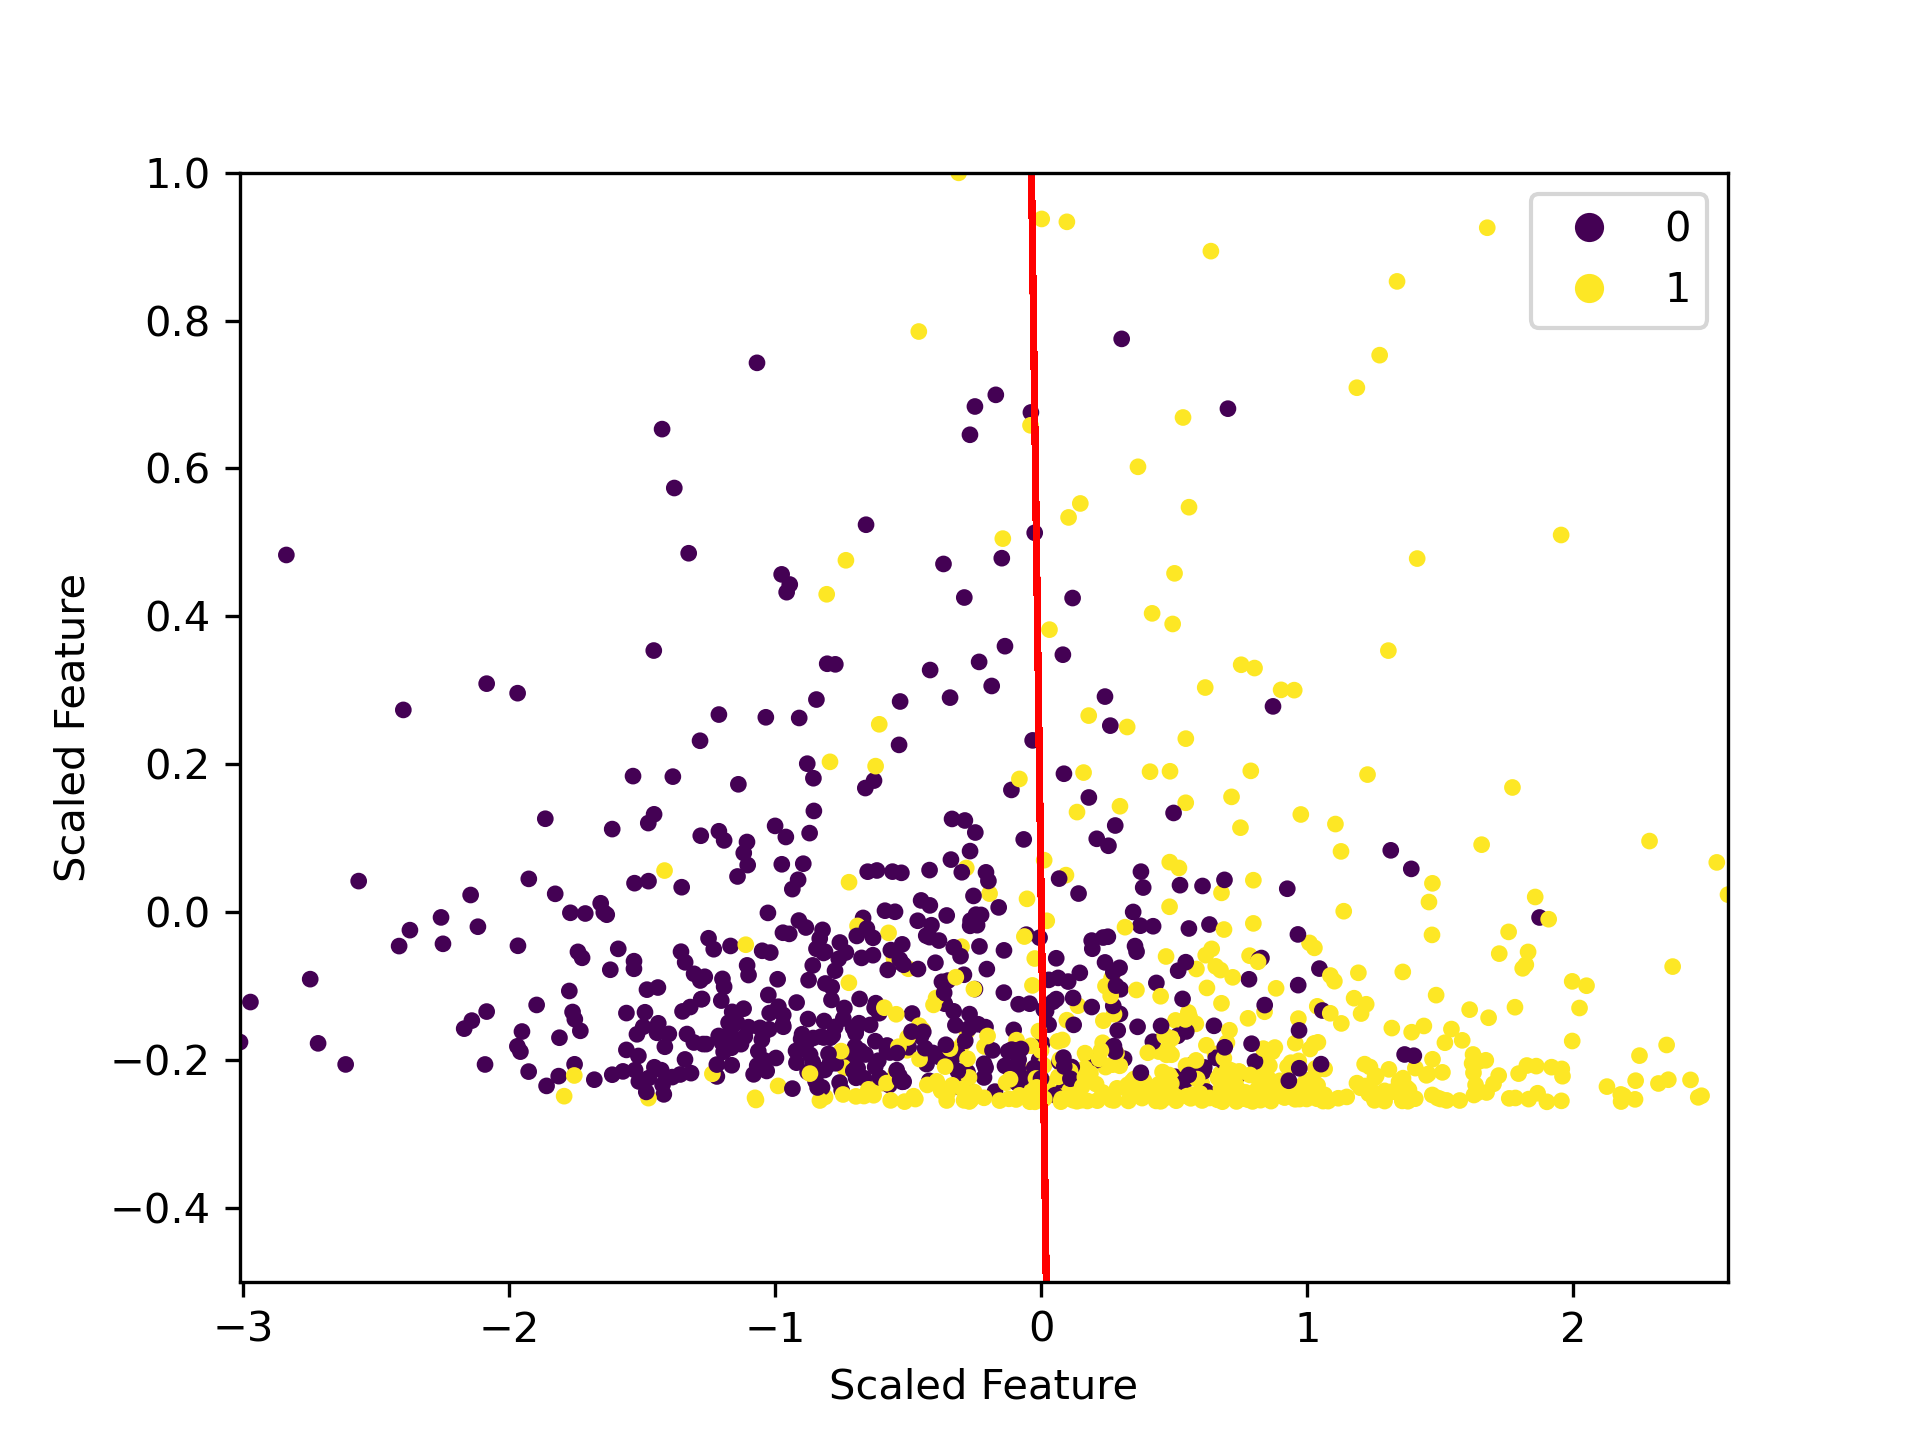
\includegraphics[width=.8\linewidth]{./plots/boundary_2-3.png}
  \caption{The 1st (x-axis) and 2nd (y-axis) rescaled features with the decision boundary. With different colors, we indicate the true labels of each point.}
  \label{fig:boun_2_3}
\end{figure}

\begin{figure}[H]
  \centering
  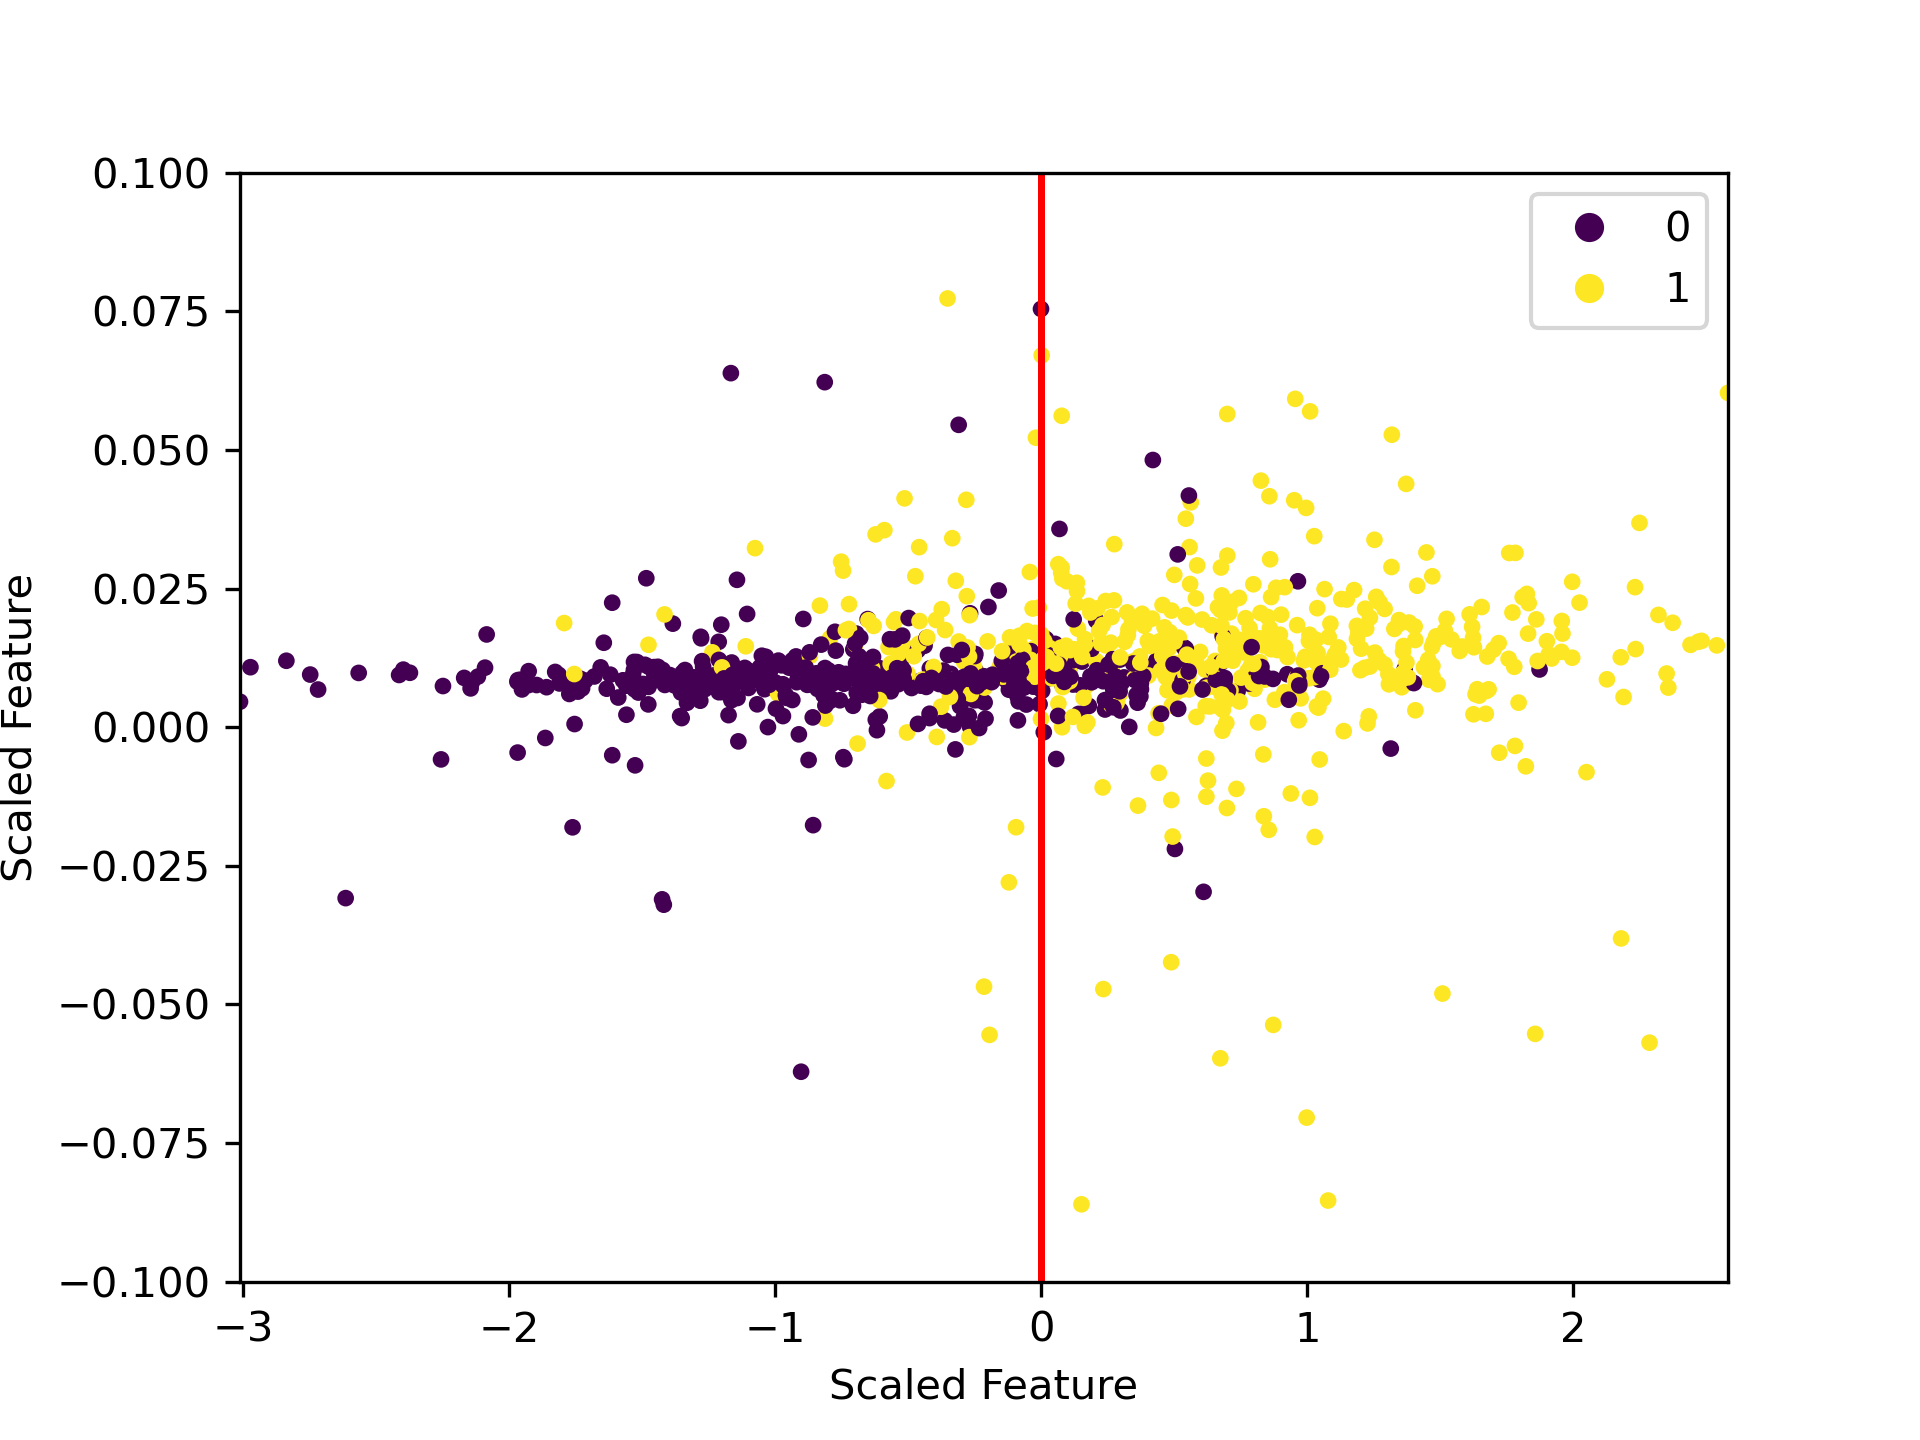
\includegraphics[width=.8\linewidth]{./plots/boundary_2-4.png}
  \caption{The 1st (x-axis) and 2nd (y-axis) rescaled features with the decision boundary. With different colors, we indicate the true labels of each point.}
  \label{fig:boun_2_4}
\end{figure}

\begin{figure}[H]
  \centering
  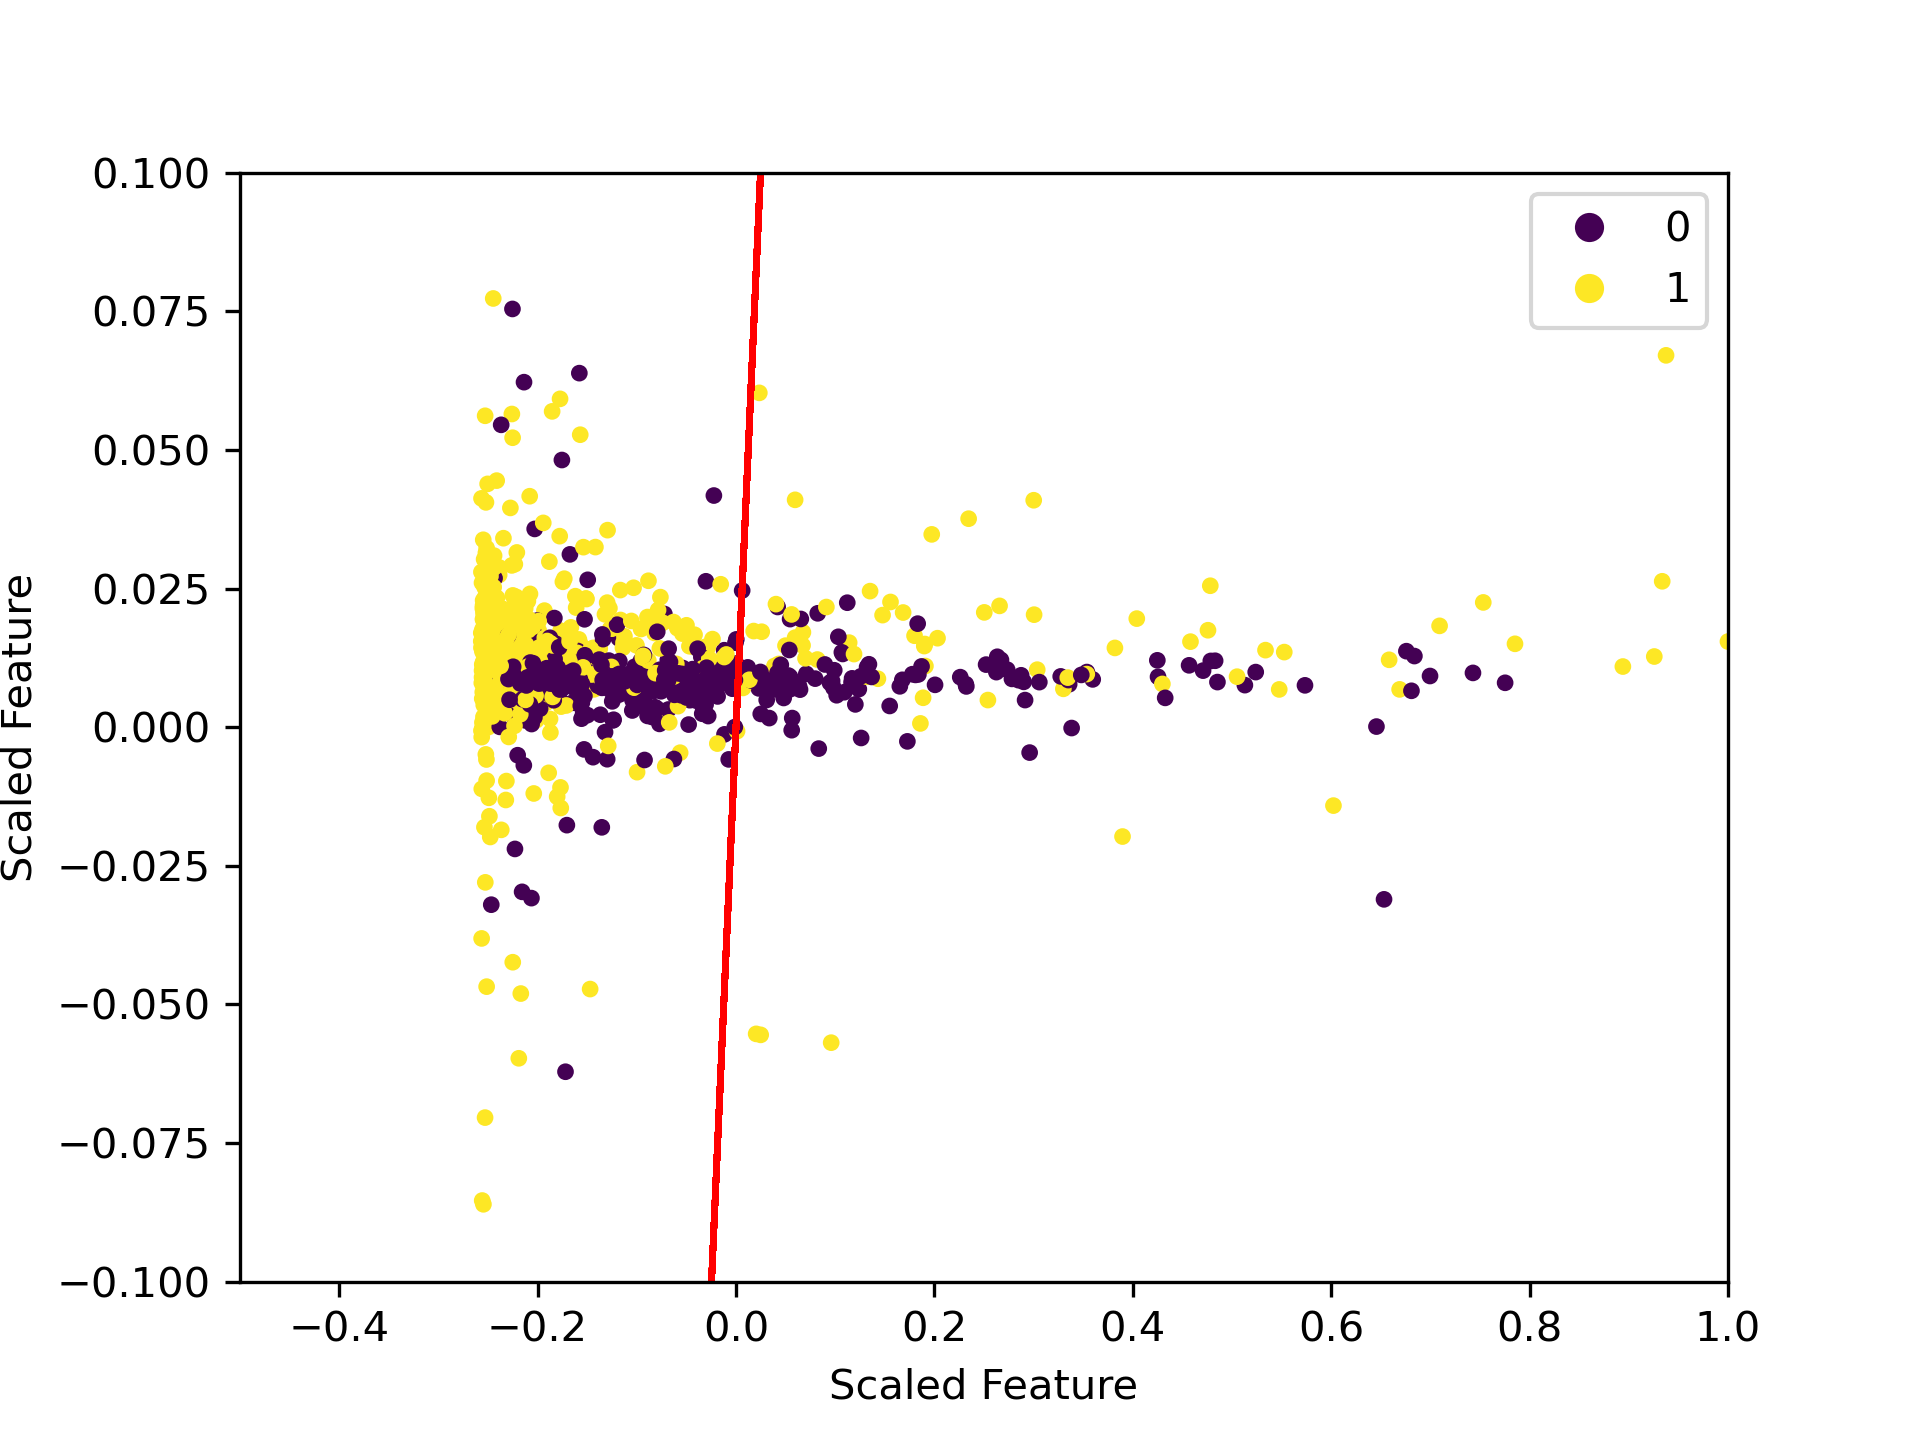
\includegraphics[width=.8\linewidth]{./plots/boundary_3-4.png}
  \caption{The 1st (x-axis) and 2nd (y-axis) rescaled features with the decision boundary. With different colors, we indicate the true labels of each point. This is the worst-performing combination of features.}
  \label{fig:boun_3_4}
\end{figure}

%references
\bibliographystyle{apacite}
\bibliography{TeX/references}


\end{document}
